\PassOptionsToPackage{unicode=true}{hyperref} % options for packages loaded elsewhere
\PassOptionsToPackage{hyphens}{url}
%
\documentclass[]{book}
\usepackage{lmodern}
\usepackage{amssymb,amsmath}
\usepackage{ifxetex,ifluatex}
\usepackage{fixltx2e} % provides \textsubscript
\ifnum 0\ifxetex 1\fi\ifluatex 1\fi=0 % if pdftex
  \usepackage[T1]{fontenc}
  \usepackage[utf8]{inputenc}
  \usepackage{textcomp} % provides euro and other symbols
\else % if luatex or xelatex
  \usepackage{unicode-math}
  \defaultfontfeatures{Ligatures=TeX,Scale=MatchLowercase}
\fi
% use upquote if available, for straight quotes in verbatim environments
\IfFileExists{upquote.sty}{\usepackage{upquote}}{}
% use microtype if available
\IfFileExists{microtype.sty}{%
\usepackage[]{microtype}
\UseMicrotypeSet[protrusion]{basicmath} % disable protrusion for tt fonts
}{}
\IfFileExists{parskip.sty}{%
\usepackage{parskip}
}{% else
\setlength{\parindent}{0pt}
\setlength{\parskip}{6pt plus 2pt minus 1pt}
}
\usepackage{hyperref}
\hypersetup{
            pdftitle={Supplemental Material for An Exploration of Exploration: Measuring the ability of lexicase selection to find obscure pathways},
            pdfauthor={Jose Guadalupe Hernandez, Alexander Lalejini, and Charles Ofria},
            pdfborder={0 0 0},
            breaklinks=true}
\urlstyle{same}  % don't use monospace font for urls
\usepackage{color}
\usepackage{fancyvrb}
\newcommand{\VerbBar}{|}
\newcommand{\VERB}{\Verb[commandchars=\\\{\}]}
\DefineVerbatimEnvironment{Highlighting}{Verbatim}{commandchars=\\\{\}}
% Add ',fontsize=\small' for more characters per line
\usepackage{framed}
\definecolor{shadecolor}{RGB}{248,248,248}
\newenvironment{Shaded}{\begin{snugshade}}{\end{snugshade}}
\newcommand{\AlertTok}[1]{\textcolor[rgb]{0.94,0.16,0.16}{#1}}
\newcommand{\AnnotationTok}[1]{\textcolor[rgb]{0.56,0.35,0.01}{\textbf{\textit{#1}}}}
\newcommand{\AttributeTok}[1]{\textcolor[rgb]{0.77,0.63,0.00}{#1}}
\newcommand{\BaseNTok}[1]{\textcolor[rgb]{0.00,0.00,0.81}{#1}}
\newcommand{\BuiltInTok}[1]{#1}
\newcommand{\CharTok}[1]{\textcolor[rgb]{0.31,0.60,0.02}{#1}}
\newcommand{\CommentTok}[1]{\textcolor[rgb]{0.56,0.35,0.01}{\textit{#1}}}
\newcommand{\CommentVarTok}[1]{\textcolor[rgb]{0.56,0.35,0.01}{\textbf{\textit{#1}}}}
\newcommand{\ConstantTok}[1]{\textcolor[rgb]{0.00,0.00,0.00}{#1}}
\newcommand{\ControlFlowTok}[1]{\textcolor[rgb]{0.13,0.29,0.53}{\textbf{#1}}}
\newcommand{\DataTypeTok}[1]{\textcolor[rgb]{0.13,0.29,0.53}{#1}}
\newcommand{\DecValTok}[1]{\textcolor[rgb]{0.00,0.00,0.81}{#1}}
\newcommand{\DocumentationTok}[1]{\textcolor[rgb]{0.56,0.35,0.01}{\textbf{\textit{#1}}}}
\newcommand{\ErrorTok}[1]{\textcolor[rgb]{0.64,0.00,0.00}{\textbf{#1}}}
\newcommand{\ExtensionTok}[1]{#1}
\newcommand{\FloatTok}[1]{\textcolor[rgb]{0.00,0.00,0.81}{#1}}
\newcommand{\FunctionTok}[1]{\textcolor[rgb]{0.00,0.00,0.00}{#1}}
\newcommand{\ImportTok}[1]{#1}
\newcommand{\InformationTok}[1]{\textcolor[rgb]{0.56,0.35,0.01}{\textbf{\textit{#1}}}}
\newcommand{\KeywordTok}[1]{\textcolor[rgb]{0.13,0.29,0.53}{\textbf{#1}}}
\newcommand{\NormalTok}[1]{#1}
\newcommand{\OperatorTok}[1]{\textcolor[rgb]{0.81,0.36,0.00}{\textbf{#1}}}
\newcommand{\OtherTok}[1]{\textcolor[rgb]{0.56,0.35,0.01}{#1}}
\newcommand{\PreprocessorTok}[1]{\textcolor[rgb]{0.56,0.35,0.01}{\textit{#1}}}
\newcommand{\RegionMarkerTok}[1]{#1}
\newcommand{\SpecialCharTok}[1]{\textcolor[rgb]{0.00,0.00,0.00}{#1}}
\newcommand{\SpecialStringTok}[1]{\textcolor[rgb]{0.31,0.60,0.02}{#1}}
\newcommand{\StringTok}[1]{\textcolor[rgb]{0.31,0.60,0.02}{#1}}
\newcommand{\VariableTok}[1]{\textcolor[rgb]{0.00,0.00,0.00}{#1}}
\newcommand{\VerbatimStringTok}[1]{\textcolor[rgb]{0.31,0.60,0.02}{#1}}
\newcommand{\WarningTok}[1]{\textcolor[rgb]{0.56,0.35,0.01}{\textbf{\textit{#1}}}}
\usepackage{longtable,booktabs}
% Fix footnotes in tables (requires footnote package)
\IfFileExists{footnote.sty}{\usepackage{footnote}\makesavenoteenv{longtable}}{}
\usepackage{graphicx,grffile}
\makeatletter
\def\maxwidth{\ifdim\Gin@nat@width>\linewidth\linewidth\else\Gin@nat@width\fi}
\def\maxheight{\ifdim\Gin@nat@height>\textheight\textheight\else\Gin@nat@height\fi}
\makeatother
% Scale images if necessary, so that they will not overflow the page
% margins by default, and it is still possible to overwrite the defaults
% using explicit options in \includegraphics[width, height, ...]{}
\setkeys{Gin}{width=\maxwidth,height=\maxheight,keepaspectratio}
\setlength{\emergencystretch}{3em}  % prevent overfull lines
\providecommand{\tightlist}{%
  \setlength{\itemsep}{0pt}\setlength{\parskip}{0pt}}
\setcounter{secnumdepth}{5}
% Redefines (sub)paragraphs to behave more like sections
\ifx\paragraph\undefined\else
\let\oldparagraph\paragraph
\renewcommand{\paragraph}[1]{\oldparagraph{#1}\mbox{}}
\fi
\ifx\subparagraph\undefined\else
\let\oldsubparagraph\subparagraph
\renewcommand{\subparagraph}[1]{\oldsubparagraph{#1}\mbox{}}
\fi

% set default figure placement to htbp
\makeatletter
\def\fps@figure{htbp}
\makeatother

\usepackage[]{natbib}
\bibliographystyle{apalike}

\title{Supplemental Material for An Exploration of Exploration: Measuring the ability of lexicase selection to find obscure pathways}
\author{Jose Guadalupe Hernandez, Alexander Lalejini, and Charles Ofria}
\date{2021-06-21}

\begin{document}
\maketitle

{
\setcounter{tocdepth}{1}
\tableofcontents
}
\hypertarget{introduction}{%
\chapter{Introduction}\label{introduction}}

This is the supplemental material associated with our 2021 GPTP contribution entitled, \emph{An Exploration of Exploration: Measuring the ability of lexicase selection to find obscure pathways}.
Preprint forthcoming.

\hypertarget{about-our-supplemental-material}{%
\section{About our supplemental material}\label{about-our-supplemental-material}}

This supplemental material is hosted on \href{https://github.com}{GitHub} using GitHub pages.
The source code and configuration files used to generate this supplemental material can be found in \href{https://github.com/jgh9094/GPTP-2021-Exploration-Of-Exploration}{this GitHub repository}.
We compiled our data analyses and supplemental documentation into this nifty web-accessible book using \href{https://bookdown.org/}{bookdown}.

Our supplemental material includes the following:

\begin{itemize}
\tightlist
\item
  TODO
\end{itemize}

\hypertarget{contributing-authors}{%
\section{Contributing authors}\label{contributing-authors}}

\begin{itemize}
\tightlist
\item
  \href{https://jgh9094.github.io/}{Jose Guadalupe Hernandez}
\item
  \href{https://lalejini.com}{Alexander Lalejini}
\item
  \href{http://ofria.com}{Charles Ofria}
\end{itemize}

\hypertarget{research-overview}{%
\section{Research overview}\label{research-overview}}

Abstract:

\begin{quote}
TODO
\end{quote}

\hypertarget{data-availability}{%
\chapter{Data Availability}\label{data-availability}}

\hypertarget{source-code}{%
\section{Source code}\label{source-code}}

The source code for this work is available on GitHub at \url{https://github.com/jgh9094/GPTP-2021-Exploration-Of-Exploration}.

\hypertarget{experimental-results}{%
\section{Experimental results}\label{experimental-results}}

The data from our experiments are available online in an OSF repository \citep{osf_data} at \url{https://osf.io/xpjft/}.

\hypertarget{compile-and-run-experiments}{%
\chapter{Compile and run experiments}\label{compile-and-run-experiments}}

Here, we provide a guide to compiling and running our experiments using our Docker image.

Please file an \href{https://github.com/jgh9094/GPTP-2021-Exploration-Of-Exploration/issues}{issue on GitHub} if something is unclear or does not work.

\hypertarget{docker}{%
\section{Docker}\label{docker}}

TODO

\hypertarget{getting-the-right-image}{%
\subsection{Getting the right image}\label{getting-the-right-image}}

\hypertarget{dockerhub}{%
\subsubsection{DockerHub}\label{dockerhub}}

\hypertarget{local-build}{%
\subsubsection{Local build}\label{local-build}}

\hypertarget{spinning-up-a-container}{%
\subsection{Spinning up a container}\label{spinning-up-a-container}}

\hypertarget{running-inside-the-container}{%
\subsection{Running inside the container}\label{running-inside-the-container}}

\hypertarget{copying-content-from-the-container}{%
\subsection{Copying content from the container}\label{copying-content-from-the-container}}

\hypertarget{tournament-selection-vs-lexicase-selection}{%
\chapter{Tournament selection vs Lexicase selection}\label{tournament-selection-vs-lexicase-selection}}

\hypertarget{overview}{%
\section{Overview}\label{overview}}

\begin{Shaded}
\begin{Highlighting}[]
\CommentTok{# Relative location of data.}
\NormalTok{working_directory <-}\StringTok{ "experiments/2021-05-27-tournament/analysis/"}
\CommentTok{# working_directory <- "./"}

\CommentTok{# Settings for visualization}
\NormalTok{cb_palette <-}\StringTok{ "Set2"}

\CommentTok{# Create directory to dump plots}
\KeywordTok{dir.create}\NormalTok{(}\KeywordTok{paste0}\NormalTok{(working_directory, }\StringTok{"imgs"}\NormalTok{), }\DataTypeTok{showWarnings=}\OtherTok{FALSE}\NormalTok{)}
\end{Highlighting}
\end{Shaded}

\hypertarget{analysis-dependencies}{%
\section{Analysis dependencies}\label{analysis-dependencies}}

\begin{Shaded}
\begin{Highlighting}[]
\KeywordTok{library}\NormalTok{(ggplot2)}
\KeywordTok{library}\NormalTok{(tidyverse)}
\KeywordTok{library}\NormalTok{(knitr)}
\KeywordTok{library}\NormalTok{(cowplot)}
\KeywordTok{library}\NormalTok{(viridis)}
\KeywordTok{library}\NormalTok{(RColorBrewer)}
\KeywordTok{library}\NormalTok{(rstatix)}
\KeywordTok{library}\NormalTok{(ggsignif)}
\KeywordTok{library}\NormalTok{(Hmisc)}
\KeywordTok{source}\NormalTok{(}\StringTok{"https://gist.githubusercontent.com/benmarwick/2a1bb0133ff568cbe28d/raw/fb53bd97121f7f9ce947837ef1a4c65a73bffb3f/geom_flat_violin.R"}\NormalTok{)}
\end{Highlighting}
\end{Shaded}

These analyses were conducted in the following computing environment:

\begin{Shaded}
\begin{Highlighting}[]
\KeywordTok{print}\NormalTok{(version)}
\end{Highlighting}
\end{Shaded}

\begin{verbatim}
##                _                           
## platform       x86_64-pc-linux-gnu         
## arch           x86_64                      
## os             linux-gnu                   
## system         x86_64, linux-gnu           
## status                                     
## major          4                           
## minor          1.0                         
## year           2021                        
## month          05                          
## day            18                          
## svn rev        80317                       
## language       R                           
## version.string R version 4.1.0 (2021-05-18)
## nickname       Camp Pontanezen
\end{verbatim}

\hypertarget{setup}{%
\section{Setup}\label{setup}}

\begin{Shaded}
\begin{Highlighting}[]
\NormalTok{data_loc <-}\StringTok{ }\KeywordTok{paste0}\NormalTok{(}
\NormalTok{  working_directory,}
  \StringTok{"data/timeseries-res-1000g.csv"}
\NormalTok{)}

\NormalTok{data <-}\StringTok{ }\KeywordTok{read.csv}\NormalTok{(data_loc, }\DataTypeTok{na.strings=}\StringTok{"NONE"}\NormalTok{)}

\NormalTok{data}\OperatorTok{$}\NormalTok{selection_name <-}\StringTok{ }\KeywordTok{factor}\NormalTok{(}
\NormalTok{  data}\OperatorTok{$}\NormalTok{selection_name,}
  \DataTypeTok{levels=}\KeywordTok{c}\NormalTok{(}\StringTok{"EpsilonLexicase"}\NormalTok{, }\StringTok{"Tournament"}\NormalTok{),}
  \DataTypeTok{labels=}\KeywordTok{c}\NormalTok{(}\StringTok{"Lexicase"}\NormalTok{, }\StringTok{"Tournament"}\NormalTok{)}
\NormalTok{)}

\NormalTok{data}\OperatorTok{$}\NormalTok{elite_trait_avg <-}
\StringTok{  }\NormalTok{data}\OperatorTok{$}\NormalTok{ele_agg_per }\OperatorTok{/}\StringTok{ }\NormalTok{data}\OperatorTok{$}\NormalTok{OBJECTIVE_CNT}
\NormalTok{data}\OperatorTok{$}\NormalTok{unique_start_positions_coverage <-}
\StringTok{  }\NormalTok{data}\OperatorTok{$}\NormalTok{uni_str_pos }\OperatorTok{/}\StringTok{ }\NormalTok{data}\OperatorTok{$}\NormalTok{OBJECTIVE_CNT}

\NormalTok{final_data <-}\StringTok{ }\KeywordTok{filter}\NormalTok{(data, evaluations}\OperatorTok{==}\KeywordTok{max}\NormalTok{(data}\OperatorTok{$}\NormalTok{evaluations))}

\CommentTok{# Labeler for stats annotations}
\NormalTok{p_label <-}\StringTok{ }\ControlFlowTok{function}\NormalTok{(p_value) \{}
\NormalTok{  threshold =}\StringTok{ }\FloatTok{0.0001}
  \ControlFlowTok{if}\NormalTok{ (p_value }\OperatorTok{<}\StringTok{ }\NormalTok{threshold) \{}
    \KeywordTok{return}\NormalTok{(}\KeywordTok{paste0}\NormalTok{(}\StringTok{"p < "}\NormalTok{, threshold))}
\NormalTok{  \} }\ControlFlowTok{else}\NormalTok{ \{}
    \KeywordTok{return}\NormalTok{(}\KeywordTok{paste0}\NormalTok{(}\StringTok{"p = "}\NormalTok{, p_value))}
\NormalTok{  \}}
\NormalTok{\}}

\CommentTok{# Significance threshold}
\NormalTok{alpha <-}\StringTok{ }\FloatTok{0.05}

\CommentTok{# Common graph variables}
\NormalTok{performance_ylim <-}\StringTok{ }\DecValTok{105}
\NormalTok{coverage_ylim <-}\StringTok{ }\FloatTok{1.0}

\CommentTok{####### misc #######}
\CommentTok{# Configure our default graphing theme}
\KeywordTok{theme_set}\NormalTok{(}\KeywordTok{theme_cowplot}\NormalTok{())}
\end{Highlighting}
\end{Shaded}

\hypertarget{exploration-diagnostic-performance}{%
\section{Exploration diagnostic performance}\label{exploration-diagnostic-performance}}

\begin{Shaded}
\begin{Highlighting}[]
\NormalTok{elite_ave_performance_fig <-}\StringTok{ }\KeywordTok{ggplot}\NormalTok{(}
\NormalTok{    data,}
    \KeywordTok{aes}\NormalTok{(}
      \DataTypeTok{x=}\NormalTok{gen,}
      \DataTypeTok{y=}\NormalTok{elite_trait_avg,}
      \DataTypeTok{color=}\NormalTok{selection_name,}
      \DataTypeTok{fill=}\NormalTok{selection_name}
\NormalTok{    )}
\NormalTok{  ) }\OperatorTok{+}
\StringTok{  }\KeywordTok{stat_summary}\NormalTok{(}\DataTypeTok{geom=}\StringTok{"line"}\NormalTok{, }\DataTypeTok{fun=}\NormalTok{mean) }\OperatorTok{+}
\StringTok{  }\KeywordTok{stat_summary}\NormalTok{(}
    \DataTypeTok{geom=}\StringTok{"ribbon"}\NormalTok{,}
    \DataTypeTok{fun.data=}\StringTok{"mean_cl_boot"}\NormalTok{,}
    \DataTypeTok{fun.args=}\KeywordTok{list}\NormalTok{(}\DataTypeTok{conf.int=}\FloatTok{0.95}\NormalTok{),}
    \DataTypeTok{alpha=}\FloatTok{0.2}\NormalTok{,}
    \DataTypeTok{linetype=}\DecValTok{0}
\NormalTok{  ) }\OperatorTok{+}
\StringTok{  }\KeywordTok{scale_y_continuous}\NormalTok{(}
    \DataTypeTok{name=}\StringTok{"Average trait performance"}\NormalTok{,}
    \DataTypeTok{limits=}\KeywordTok{c}\NormalTok{(}\DecValTok{0}\NormalTok{, performance_ylim)}
\NormalTok{  ) }\OperatorTok{+}
\StringTok{  }\KeywordTok{scale_x_continuous}\NormalTok{(}
    \DataTypeTok{name=}\StringTok{"Generation"}
\NormalTok{  ) }\OperatorTok{+}
\StringTok{  }\KeywordTok{scale_fill_brewer}\NormalTok{(}
    \DataTypeTok{name=}\StringTok{"Selection"}\NormalTok{,}
    \DataTypeTok{limits=}\KeywordTok{c}\NormalTok{(}\StringTok{"Lexicase"}\NormalTok{, }\StringTok{"Tournament"}\NormalTok{),}
    \DataTypeTok{labels=}\KeywordTok{c}\NormalTok{(}\StringTok{"Lexicase"}\NormalTok{, }\StringTok{"Tournament"}\NormalTok{),}
    \DataTypeTok{palette=}\NormalTok{cb_palette}
\NormalTok{  ) }\OperatorTok{+}
\StringTok{  }\KeywordTok{scale_color_brewer}\NormalTok{(}
    \DataTypeTok{name=}\StringTok{"Selection"}\NormalTok{,}
    \DataTypeTok{limits=}\KeywordTok{c}\NormalTok{(}\StringTok{"Lexicase"}\NormalTok{, }\StringTok{"Tournament"}\NormalTok{),}
    \DataTypeTok{labels=}\KeywordTok{c}\NormalTok{(}\StringTok{"Lexicase"}\NormalTok{, }\StringTok{"Tournament"}\NormalTok{),}
    \DataTypeTok{palette=}\NormalTok{cb_palette}
\NormalTok{  )}
\NormalTok{elite_ave_performance_fig}
\end{Highlighting}
\end{Shaded}

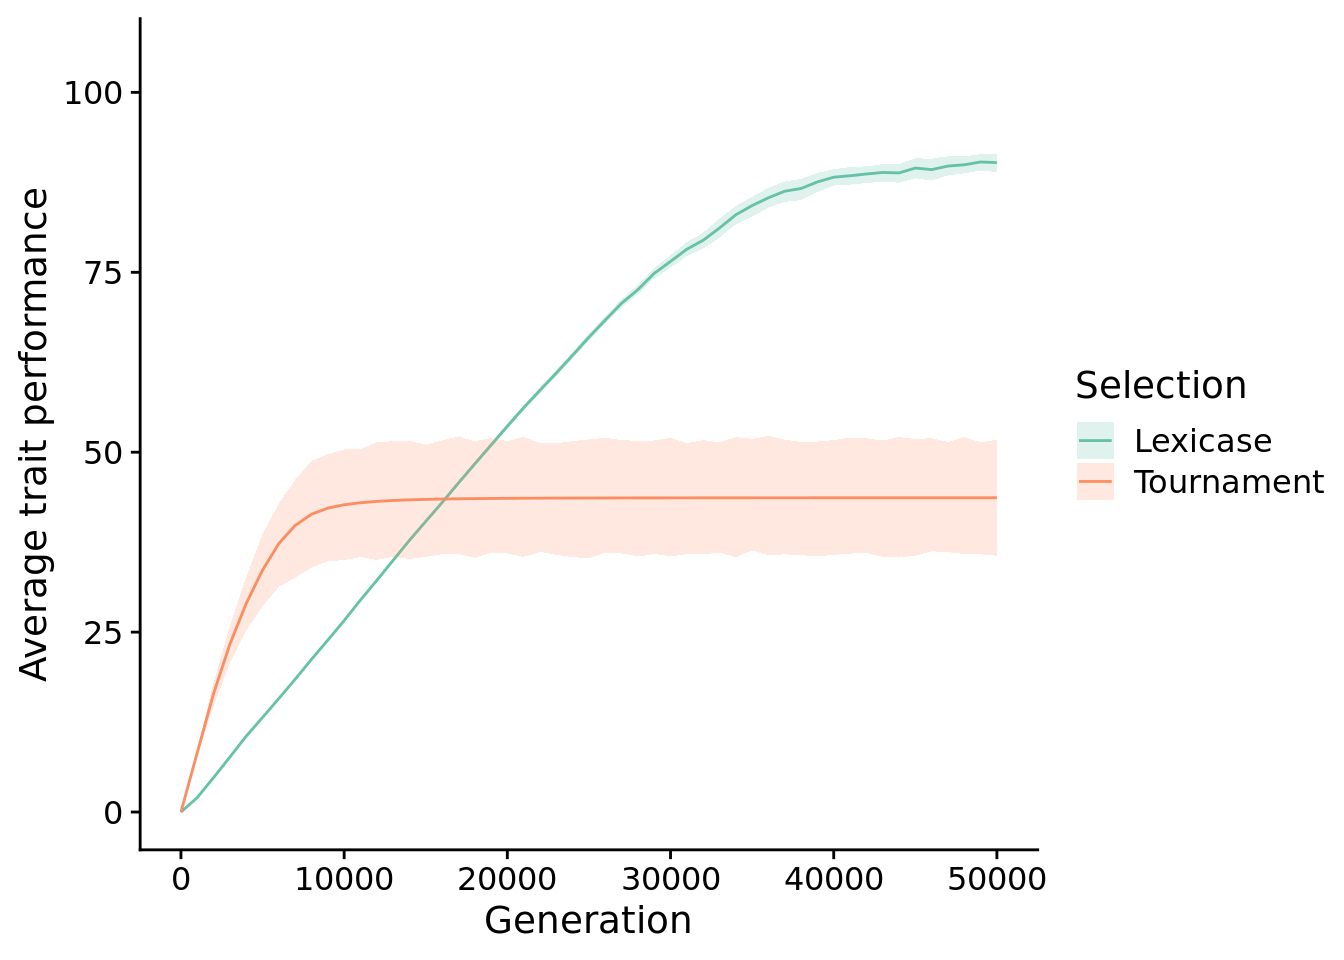
\includegraphics{supplemental-material_files/figure-latex/unnamed-chunk-5-1.pdf}

\hypertarget{final-performance}{%
\section{Final Performance}\label{final-performance}}

\begin{Shaded}
\begin{Highlighting}[]
\CommentTok{# Compute manual labels for geom_signif}
\NormalTok{stat.test <-}\StringTok{ }\NormalTok{final_data }\OperatorTok
\StringTok{  }\KeywordTok{wilcox_test}\NormalTok{(elite_trait_avg }\OperatorTok{~}\StringTok{ }\NormalTok{selection_name) }\OperatorTok
\StringTok{  }\KeywordTok{adjust_pvalue}\NormalTok{(}\DataTypeTok{method =} \StringTok{"bonferroni"}\NormalTok{) }\OperatorTok
\StringTok{  }\KeywordTok{add_significance}\NormalTok{() }\OperatorTok
\StringTok{  }\KeywordTok{add_xy_position}\NormalTok{(}\DataTypeTok{x=}\StringTok{"selection_name"}\NormalTok{,}\DataTypeTok{step.increase=}\DecValTok{1}\NormalTok{)}
\NormalTok{stat.test}\OperatorTok{$}\NormalTok{manual_position <-}\StringTok{ }\NormalTok{stat.test}\OperatorTok{$}\NormalTok{y.position }\OperatorTok{*}\StringTok{ }\FloatTok{1.05}
\NormalTok{stat.test}\OperatorTok{$}\NormalTok{label <-}\StringTok{ }\KeywordTok{mapply}\NormalTok{(p_label,stat.test}\OperatorTok{$}\NormalTok{p.adj)}
\end{Highlighting}
\end{Shaded}

\begin{Shaded}
\begin{Highlighting}[]
\NormalTok{elite_final_performance_fig <-}\StringTok{ }\KeywordTok{ggplot}\NormalTok{(}
\NormalTok{    final_data,}
    \KeywordTok{aes}\NormalTok{(}
      \DataTypeTok{x=}\NormalTok{selection_name,}
      \DataTypeTok{y=}\NormalTok{elite_trait_avg,}
      \DataTypeTok{fill=}\NormalTok{selection_name}
\NormalTok{    )}
\NormalTok{  ) }\OperatorTok{+}
\StringTok{  }\KeywordTok{geom_flat_violin}\NormalTok{(}
    \DataTypeTok{position =} \KeywordTok{position_nudge}\NormalTok{(}\DataTypeTok{x =} \FloatTok{.2}\NormalTok{, }\DataTypeTok{y =} \DecValTok{0}\NormalTok{),}
    \DataTypeTok{alpha =} \FloatTok{.8}\NormalTok{,}
    \DataTypeTok{scale=}\StringTok{"width"}
\NormalTok{  ) }\OperatorTok{+}
\StringTok{  }\KeywordTok{geom_point}\NormalTok{(}
    \DataTypeTok{mapping=}\KeywordTok{aes}\NormalTok{(}\DataTypeTok{color=}\NormalTok{selection_name),}
    \DataTypeTok{position =} \KeywordTok{position_jitter}\NormalTok{(}\DataTypeTok{width =} \FloatTok{.15}\NormalTok{),}
    \DataTypeTok{size =} \FloatTok{.5}\NormalTok{,}
    \DataTypeTok{alpha =} \FloatTok{0.8}
\NormalTok{  ) }\OperatorTok{+}
\StringTok{  }\KeywordTok{geom_boxplot}\NormalTok{(}
    \DataTypeTok{width =} \FloatTok{.1}\NormalTok{,}
    \DataTypeTok{outlier.shape =} \OtherTok{NA}\NormalTok{,}
    \DataTypeTok{alpha =} \FloatTok{0.5}
\NormalTok{  ) }\OperatorTok{+}
\StringTok{  }\KeywordTok{scale_y_continuous}\NormalTok{(}
    \DataTypeTok{name=}\StringTok{"Average trait performance"}\NormalTok{,}
    \DataTypeTok{limits=}\KeywordTok{c}\NormalTok{(}\DecValTok{0}\NormalTok{, performance_ylim)}
\NormalTok{  ) }\OperatorTok{+}
\StringTok{  }\KeywordTok{scale_x_discrete}\NormalTok{(}
    \DataTypeTok{name=}\StringTok{"Selection"}\NormalTok{,}
    \DataTypeTok{limits=}\KeywordTok{c}\NormalTok{(}\StringTok{"Lexicase"}\NormalTok{, }\StringTok{"Tournament"}\NormalTok{),}
    \DataTypeTok{labels=}\KeywordTok{c}\NormalTok{(}\StringTok{"Lexicase"}\NormalTok{, }\StringTok{"Tournament"}\NormalTok{),}
\NormalTok{  ) }\OperatorTok{+}
\StringTok{  }\KeywordTok{scale_fill_brewer}\NormalTok{(}
    \DataTypeTok{name=}\StringTok{"Selection"}\NormalTok{,}
    \DataTypeTok{palette=}\NormalTok{cb_palette,}
    \DataTypeTok{limits=}\KeywordTok{c}\NormalTok{(}\StringTok{"Lexicase"}\NormalTok{, }\StringTok{"Tournament"}\NormalTok{),}
    \DataTypeTok{labels=}\KeywordTok{c}\NormalTok{(}\StringTok{"Lexicase"}\NormalTok{, }\StringTok{"Tournament"}\NormalTok{),}
\NormalTok{  ) }\OperatorTok{+}
\StringTok{  }\KeywordTok{scale_color_brewer}\NormalTok{(}
    \DataTypeTok{name=}\StringTok{"Selection"}\NormalTok{,}
    \DataTypeTok{palette=}\NormalTok{cb_palette,}
    \DataTypeTok{limits=}\KeywordTok{c}\NormalTok{(}\StringTok{"Lexicase"}\NormalTok{, }\StringTok{"Tournament"}\NormalTok{),}
    \DataTypeTok{labels=}\KeywordTok{c}\NormalTok{(}\StringTok{"Lexicase"}\NormalTok{, }\StringTok{"Tournament"}\NormalTok{),}
\NormalTok{  ) }\OperatorTok{+}
\StringTok{  }\KeywordTok{labs}\NormalTok{(}
    \DataTypeTok{subtitle=}\KeywordTok{paste0}\NormalTok{(}
      \StringTok{"Kruskal-Wallis, "}\NormalTok{,}
      \KeywordTok{p_label}\NormalTok{(}
        \KeywordTok{signif}\NormalTok{(}
          \KeywordTok{kruskal.test}\NormalTok{(}
            \DataTypeTok{formula=}\NormalTok{elite_trait_avg}\OperatorTok{~}\NormalTok{selection_name,}
            \DataTypeTok{data=}\NormalTok{final_data)}\OperatorTok{$}\NormalTok{p.value,}\DataTypeTok{digits=}\DecValTok{4}
\NormalTok{        )}
\NormalTok{      )}
\NormalTok{    )}
\NormalTok{  ) }\OperatorTok{+}
\StringTok{  }\NormalTok{ggsignif}\OperatorTok{::}\KeywordTok{geom_signif}\NormalTok{(}
    \DataTypeTok{data=}\KeywordTok{filter}\NormalTok{(stat.test, p.adj }\OperatorTok{<=}\StringTok{ }\NormalTok{alpha),}
    \KeywordTok{aes}\NormalTok{(}
      \DataTypeTok{xmin=}\NormalTok{group1,}
      \DataTypeTok{xmax=}\NormalTok{group2,}
      \DataTypeTok{annotations=}\NormalTok{label,}
      \DataTypeTok{y_position=}\NormalTok{manual_position}
\NormalTok{    ),}
    \DataTypeTok{manual=}\OtherTok{TRUE}\NormalTok{,}
    \DataTypeTok{inherit.aes=}\OtherTok{FALSE}
\NormalTok{  ) }\OperatorTok{+}
\StringTok{  }\KeywordTok{theme}\NormalTok{(}
    \DataTypeTok{legend.position=}\StringTok{"none"}
\NormalTok{  )}
\end{Highlighting}
\end{Shaded}

\begin{verbatim}
## Warning: Ignoring unknown aesthetics: xmin, xmax, annotations, y_position
\end{verbatim}

\begin{Shaded}
\begin{Highlighting}[]
\NormalTok{elite_final_performance_fig}
\end{Highlighting}
\end{Shaded}

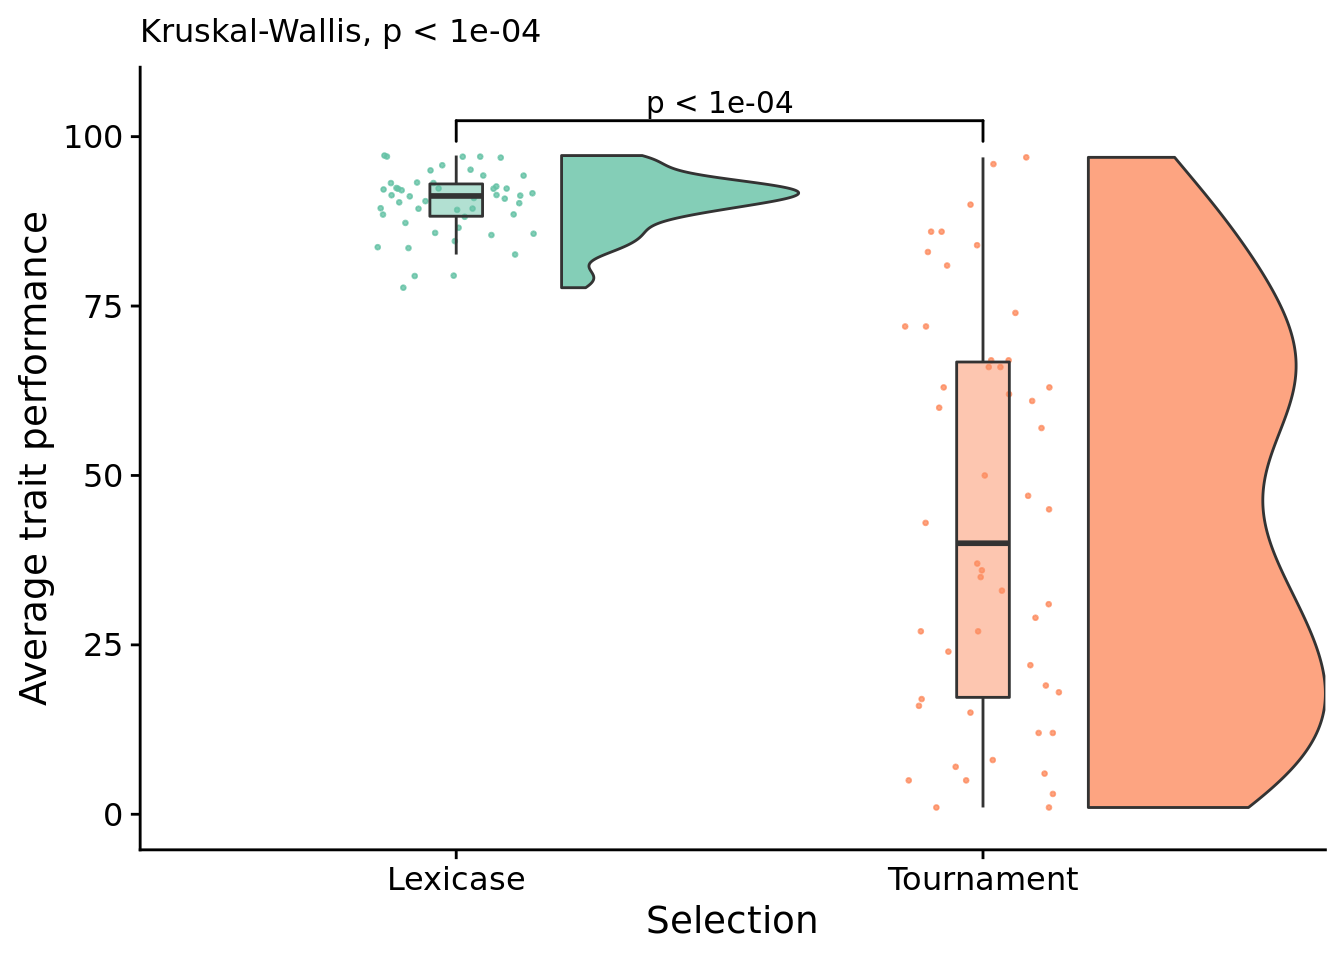
\includegraphics{supplemental-material_files/figure-latex/unnamed-chunk-7-1.pdf}

\begin{tabular}{l|l|l|r|r|r|r|r|l|r|l|r|r|r|l}
\hline
.y. & group1 & group2 & n1 & n2 & statistic & p & p.adj & p.adj.signif & y.position & groups & xmin & xmax & manual\_position & label\\
\hline
elite\_trait\_avg & Lexicase & Tournament & 50 & 50 & 2357 & 0 & 0 & **** & 97.477 & Lexicase  , Tournament & 1 & 2 & 102.3508 & p < 1e-04\\
\hline
\end{tabular}

\hypertarget{unique-starting-positions}{%
\section{Unique starting positions}\label{unique-starting-positions}}

\begin{Shaded}
\begin{Highlighting}[]
\KeywordTok{ggplot}\NormalTok{(data, }\KeywordTok{aes}\NormalTok{(}\DataTypeTok{x=}\NormalTok{gen, }\DataTypeTok{y=}\NormalTok{uni_str_pos, }\DataTypeTok{color=}\NormalTok{selection_name)) }\OperatorTok{+}
\StringTok{  }\KeywordTok{stat_summary}\NormalTok{(}\DataTypeTok{geom=}\StringTok{"line"}\NormalTok{, }\DataTypeTok{fun=}\NormalTok{mean) }\OperatorTok{+}
\StringTok{  }\KeywordTok{stat_summary}\NormalTok{(}
    \DataTypeTok{geom=}\StringTok{"ribbon"}\NormalTok{,}
    \DataTypeTok{fun.data=}\StringTok{"mean_cl_boot"}\NormalTok{,}
    \DataTypeTok{fun.args=}\KeywordTok{list}\NormalTok{(}\DataTypeTok{conf.int=}\FloatTok{0.95}\NormalTok{),}
    \DataTypeTok{alpha=}\FloatTok{0.2}\NormalTok{,}
    \DataTypeTok{linetype=}\DecValTok{0}
\NormalTok{  ) }\OperatorTok{+}
\StringTok{  }\KeywordTok{scale_y_continuous}\NormalTok{(}
    \DataTypeTok{name=}\StringTok{"Unique activation positions (population)"}\NormalTok{,}
    \DataTypeTok{limits=}\KeywordTok{c}\NormalTok{(}\DecValTok{0}\NormalTok{, }\DecValTok{100}\NormalTok{)}
\NormalTok{  ) }\OperatorTok{+}
\StringTok{  }\KeywordTok{scale_x_continuous}\NormalTok{(}
    \DataTypeTok{name=}\StringTok{"Generation"}
\NormalTok{  )}
\end{Highlighting}
\end{Shaded}

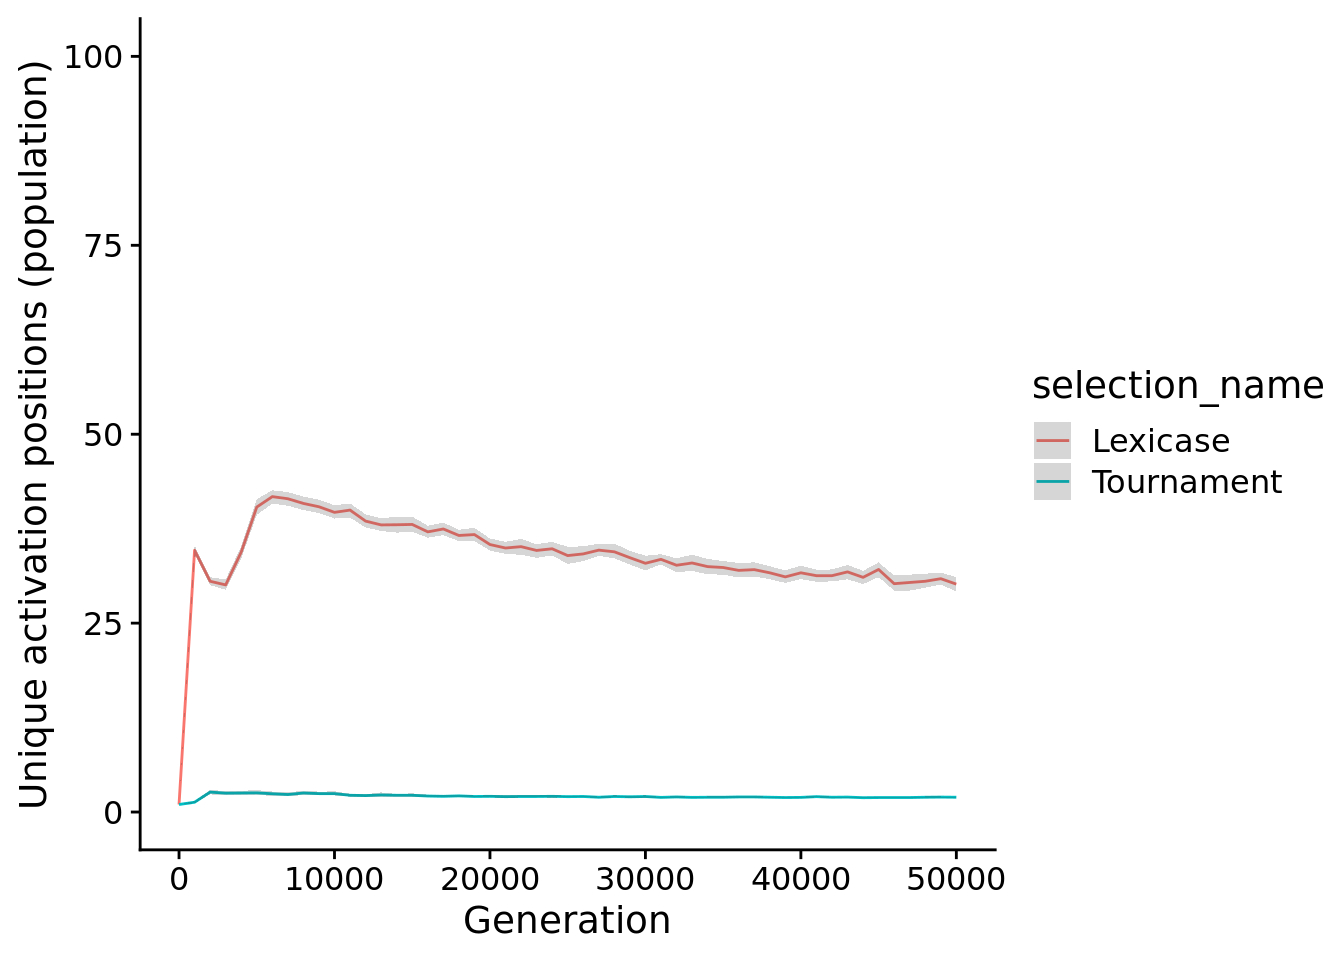
\includegraphics{supplemental-material_files/figure-latex/unnamed-chunk-9-1.pdf}

Different cardinalities have numbers of possible starting positions, so next, we look at the proportion of starting positions (out of all possible) maintained by populations.

\begin{Shaded}
\begin{Highlighting}[]
\NormalTok{unique_start_position_coverage_fig <-}\StringTok{ }\KeywordTok{ggplot}\NormalTok{(}
\NormalTok{    data,}
    \KeywordTok{aes}\NormalTok{(}
      \DataTypeTok{x=}\NormalTok{gen,}
      \DataTypeTok{y=}\NormalTok{unique_start_positions_coverage,}
      \DataTypeTok{color=}\NormalTok{selection_name,}
      \DataTypeTok{fill=}\NormalTok{selection_name}
\NormalTok{    )}
\NormalTok{  ) }\OperatorTok{+}
\StringTok{  }\KeywordTok{stat_summary}\NormalTok{(}\DataTypeTok{geom=}\StringTok{"line"}\NormalTok{, }\DataTypeTok{fun=}\NormalTok{mean) }\OperatorTok{+}
\StringTok{  }\KeywordTok{stat_summary}\NormalTok{(}
    \DataTypeTok{geom=}\StringTok{"ribbon"}\NormalTok{,}
    \DataTypeTok{fun.data=}\StringTok{"mean_cl_boot"}\NormalTok{,}
    \DataTypeTok{fun.args=}\KeywordTok{list}\NormalTok{(}\DataTypeTok{conf.int=}\FloatTok{0.95}\NormalTok{),}
    \DataTypeTok{alpha=}\FloatTok{0.2}\NormalTok{,}
    \DataTypeTok{linetype=}\DecValTok{0}
\NormalTok{  ) }\OperatorTok{+}
\StringTok{  }\KeywordTok{scale_y_continuous}\NormalTok{(}
    \DataTypeTok{name=}\StringTok{"Activation position coverage"}\NormalTok{,}
    \DataTypeTok{limit=}\KeywordTok{c}\NormalTok{(}\DecValTok{0}\NormalTok{, coverage_ylim)}
\NormalTok{  ) }\OperatorTok{+}
\StringTok{  }\KeywordTok{scale_x_continuous}\NormalTok{(}
    \DataTypeTok{name=}\StringTok{"Generation"}
\NormalTok{  ) }\OperatorTok{+}
\StringTok{  }\KeywordTok{scale_fill_brewer}\NormalTok{(}
    \DataTypeTok{name=}\StringTok{"Selection"}\NormalTok{,}
    \DataTypeTok{limits=}\KeywordTok{c}\NormalTok{(}\StringTok{"Lexicase"}\NormalTok{, }\StringTok{"Tournament"}\NormalTok{),}
    \DataTypeTok{labels=}\KeywordTok{c}\NormalTok{(}\StringTok{"Lexicase"}\NormalTok{, }\StringTok{"Tournament"}\NormalTok{),}
    \DataTypeTok{palette=}\NormalTok{cb_palette}
\NormalTok{  ) }\OperatorTok{+}
\StringTok{  }\KeywordTok{scale_color_brewer}\NormalTok{(}
    \DataTypeTok{name=}\StringTok{"Selection"}\NormalTok{,}
    \DataTypeTok{limits=}\KeywordTok{c}\NormalTok{(}\StringTok{"Lexicase"}\NormalTok{, }\StringTok{"Tournament"}\NormalTok{),}
    \DataTypeTok{labels=}\KeywordTok{c}\NormalTok{(}\StringTok{"Lexicase"}\NormalTok{, }\StringTok{"Tournament"}\NormalTok{),}
    \DataTypeTok{palette=}\NormalTok{cb_palette}
\NormalTok{  )}
\NormalTok{unique_start_position_coverage_fig}
\end{Highlighting}
\end{Shaded}

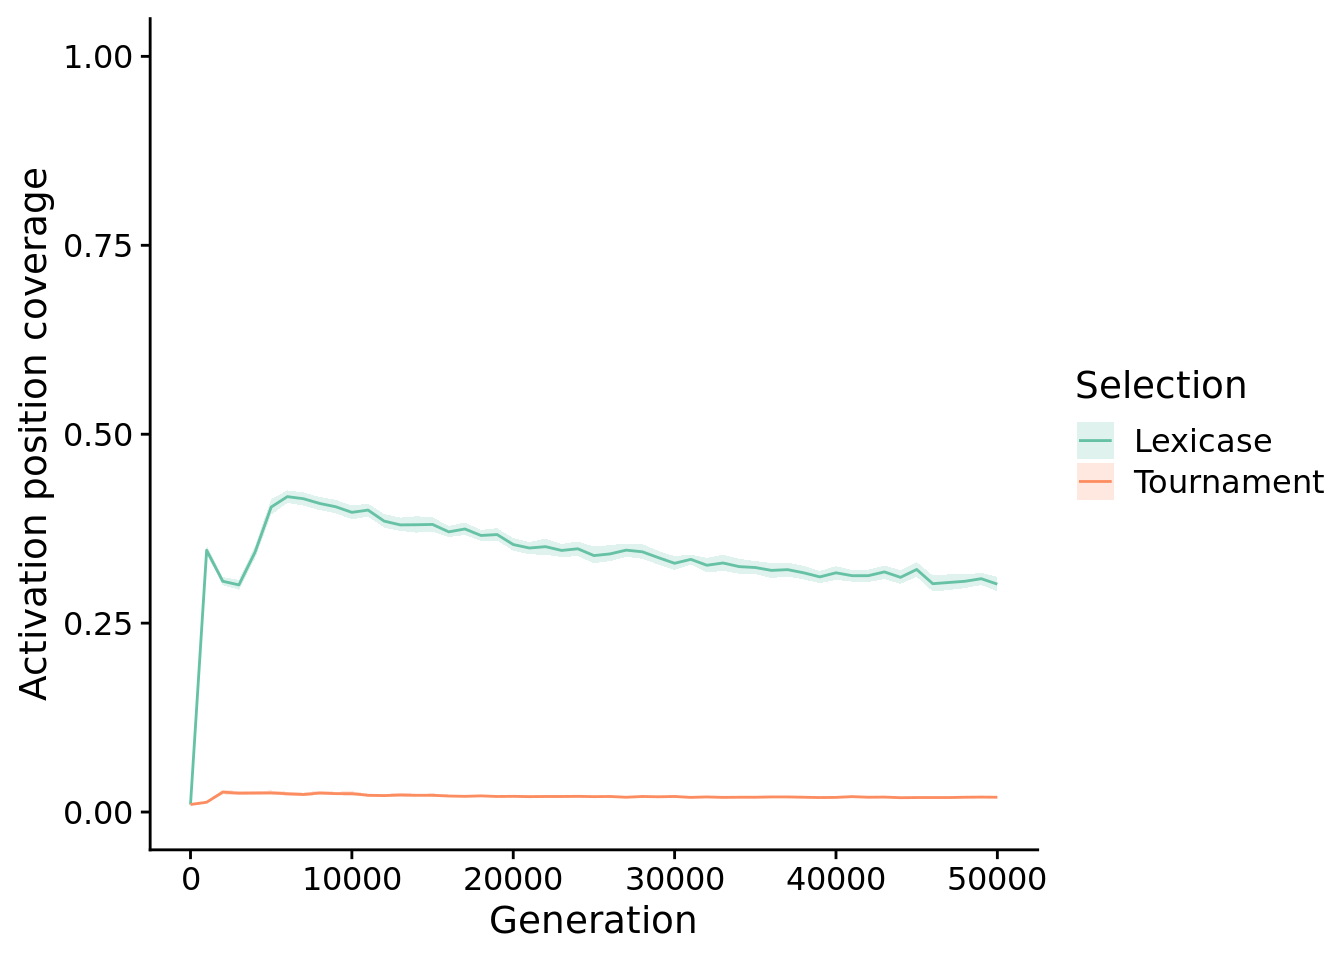
\includegraphics{supplemental-material_files/figure-latex/unnamed-chunk-10-1.pdf}

\hypertarget{final-starting-position-coverage}{%
\subsection{Final starting position Coverage}\label{final-starting-position-coverage}}

\begin{Shaded}
\begin{Highlighting}[]
\CommentTok{# Compute manual labels for geom_signif}
\NormalTok{stat.test <-}\StringTok{ }\NormalTok{final_data }\OperatorTok
\StringTok{  }\KeywordTok{wilcox_test}\NormalTok{(unique_start_positions_coverage }\OperatorTok{~}\StringTok{ }\NormalTok{selection_name) }\OperatorTok
\StringTok{  }\KeywordTok{adjust_pvalue}\NormalTok{(}\DataTypeTok{method =} \StringTok{"bonferroni"}\NormalTok{) }\OperatorTok
\StringTok{  }\KeywordTok{add_significance}\NormalTok{() }\OperatorTok
\StringTok{  }\KeywordTok{add_xy_position}\NormalTok{(}\DataTypeTok{x=}\StringTok{"selection_name"}\NormalTok{,}\DataTypeTok{step.increase=}\DecValTok{1}\NormalTok{)}
\NormalTok{stat.test}\OperatorTok{$}\NormalTok{manual_position <-}\StringTok{ }\NormalTok{stat.test}\OperatorTok{$}\NormalTok{y.position }\OperatorTok{*}\StringTok{ }\FloatTok{1.05}
\NormalTok{stat.test}\OperatorTok{$}\NormalTok{label <-}\StringTok{ }\KeywordTok{mapply}\NormalTok{(p_label,stat.test}\OperatorTok{$}\NormalTok{p.adj)}
\end{Highlighting}
\end{Shaded}

\begin{Shaded}
\begin{Highlighting}[]
\NormalTok{unique_start_positions_coverage_final_fig <-}\StringTok{ }\KeywordTok{ggplot}\NormalTok{(}
\NormalTok{    final_data,}
    \KeywordTok{aes}\NormalTok{(}
      \DataTypeTok{x=}\NormalTok{selection_name,}
      \DataTypeTok{y=}\NormalTok{unique_start_positions_coverage,}
      \DataTypeTok{fill=}\NormalTok{selection_name}
\NormalTok{    )}
\NormalTok{  ) }\OperatorTok{+}
\StringTok{  }\KeywordTok{geom_flat_violin}\NormalTok{(}
    \DataTypeTok{position =} \KeywordTok{position_nudge}\NormalTok{(}\DataTypeTok{x =} \FloatTok{.2}\NormalTok{, }\DataTypeTok{y =} \DecValTok{0}\NormalTok{),}
    \DataTypeTok{alpha =} \FloatTok{.8}\NormalTok{,}
    \DataTypeTok{scale=}\StringTok{"width"}
\NormalTok{  ) }\OperatorTok{+}
\StringTok{  }\KeywordTok{geom_point}\NormalTok{(}
    \DataTypeTok{mapping=}\KeywordTok{aes}\NormalTok{(}\DataTypeTok{color=}\NormalTok{selection_name),}
    \DataTypeTok{position =} \KeywordTok{position_jitter}\NormalTok{(}\DataTypeTok{width =} \FloatTok{.15}\NormalTok{),}
    \DataTypeTok{size =} \FloatTok{.5}\NormalTok{,}
    \DataTypeTok{alpha =} \FloatTok{0.8}
\NormalTok{  ) }\OperatorTok{+}
\StringTok{  }\KeywordTok{geom_boxplot}\NormalTok{(}
    \DataTypeTok{width =} \FloatTok{.1}\NormalTok{,}
    \DataTypeTok{outlier.shape =} \OtherTok{NA}\NormalTok{,}
    \DataTypeTok{alpha =} \FloatTok{0.5}
\NormalTok{  ) }\OperatorTok{+}
\StringTok{  }\KeywordTok{scale_y_continuous}\NormalTok{(}
    \DataTypeTok{name=}\StringTok{"Activation position coverage"}\NormalTok{,}
    \DataTypeTok{limits=}\KeywordTok{c}\NormalTok{(}\DecValTok{0}\NormalTok{, coverage_ylim)}
\NormalTok{  ) }\OperatorTok{+}
\StringTok{  }\KeywordTok{scale_x_discrete}\NormalTok{(}
    \DataTypeTok{name=}\StringTok{"Selection"}\NormalTok{,}
    \DataTypeTok{limits=}\KeywordTok{c}\NormalTok{(}\StringTok{"Lexicase"}\NormalTok{, }\StringTok{"Tournament"}\NormalTok{),}
    \DataTypeTok{labels=}\KeywordTok{c}\NormalTok{(}\StringTok{"Lexicase"}\NormalTok{, }\StringTok{"Tournament"}\NormalTok{),}
\NormalTok{  ) }\OperatorTok{+}
\StringTok{  }\KeywordTok{scale_fill_brewer}\NormalTok{(}
    \DataTypeTok{name=}\StringTok{"Selection"}\NormalTok{,}
    \DataTypeTok{palette=}\NormalTok{cb_palette,}
    \DataTypeTok{limits=}\KeywordTok{c}\NormalTok{(}\StringTok{"Lexicase"}\NormalTok{, }\StringTok{"Tournament"}\NormalTok{),}
    \DataTypeTok{labels=}\KeywordTok{c}\NormalTok{(}\StringTok{"Lexicase"}\NormalTok{, }\StringTok{"Tournament"}\NormalTok{),}
\NormalTok{  ) }\OperatorTok{+}
\StringTok{  }\KeywordTok{scale_color_brewer}\NormalTok{(}
    \DataTypeTok{name=}\StringTok{"Selection"}\NormalTok{,}
    \DataTypeTok{palette=}\NormalTok{cb_palette,}
    \DataTypeTok{limits=}\KeywordTok{c}\NormalTok{(}\StringTok{"Lexicase"}\NormalTok{, }\StringTok{"Tournament"}\NormalTok{),}
    \DataTypeTok{labels=}\KeywordTok{c}\NormalTok{(}\StringTok{"Lexicase"}\NormalTok{, }\StringTok{"Tournament"}\NormalTok{),}
\NormalTok{  ) }\OperatorTok{+}
\StringTok{  }\KeywordTok{labs}\NormalTok{(}
    \DataTypeTok{subtitle=}\KeywordTok{paste0}\NormalTok{(}
      \StringTok{"Kruskal-Wallis, "}\NormalTok{,}
      \KeywordTok{p_label}\NormalTok{(}
        \KeywordTok{signif}\NormalTok{(}
          \KeywordTok{kruskal.test}\NormalTok{(}
            \DataTypeTok{formula=}\NormalTok{unique_start_positions_coverage}\OperatorTok{~}\NormalTok{selection_name,}
            \DataTypeTok{data=}\NormalTok{final_data)}\OperatorTok{$}\NormalTok{p.value,}\DataTypeTok{digits=}\DecValTok{4}
\NormalTok{        )}
\NormalTok{      )}
\NormalTok{    )}
\NormalTok{  ) }\OperatorTok{+}
\StringTok{  }\NormalTok{ggsignif}\OperatorTok{::}\KeywordTok{geom_signif}\NormalTok{(}
    \DataTypeTok{data=}\KeywordTok{filter}\NormalTok{(stat.test, p.adj }\OperatorTok{<=}\StringTok{ }\NormalTok{alpha),}
    \KeywordTok{aes}\NormalTok{(}
      \DataTypeTok{xmin=}\NormalTok{group1,}
      \DataTypeTok{xmax=}\NormalTok{group2,}
      \DataTypeTok{annotations=}\NormalTok{label,}
      \DataTypeTok{y_position=}\NormalTok{manual_position}
\NormalTok{    ),}
    \DataTypeTok{manual=}\OtherTok{TRUE}\NormalTok{,}
    \DataTypeTok{inherit.aes=}\OtherTok{FALSE}
\NormalTok{  ) }\OperatorTok{+}
\StringTok{  }\KeywordTok{theme}\NormalTok{(}
    \DataTypeTok{legend.position=}\StringTok{"none"}
\NormalTok{  )}
\end{Highlighting}
\end{Shaded}

\begin{verbatim}
## Warning: Ignoring unknown aesthetics: xmin, xmax, annotations, y_position
\end{verbatim}

\begin{Shaded}
\begin{Highlighting}[]
\NormalTok{unique_start_positions_coverage_final_fig}
\end{Highlighting}
\end{Shaded}

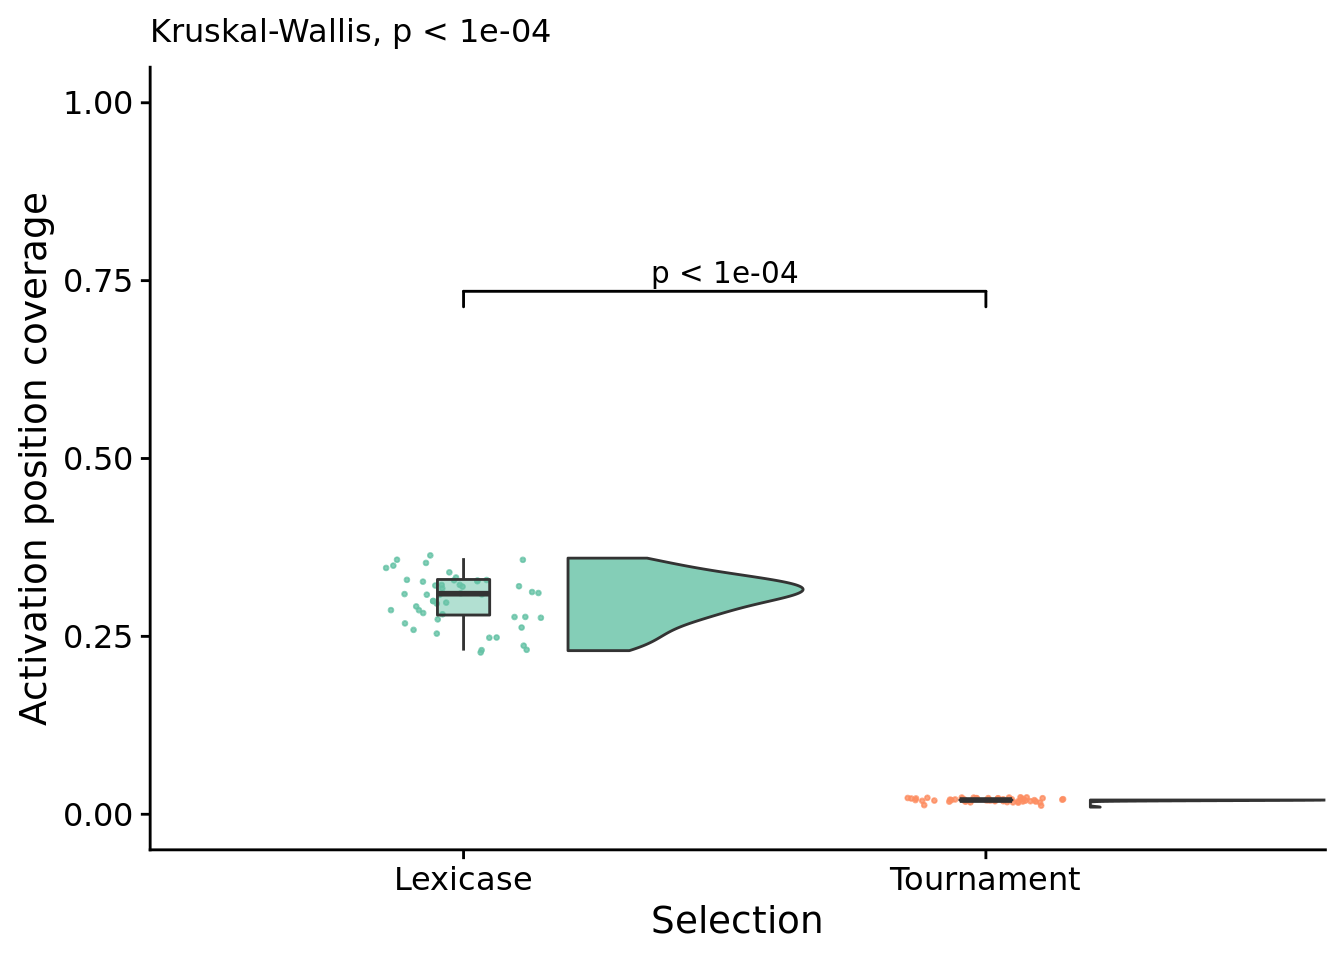
\includegraphics{supplemental-material_files/figure-latex/unnamed-chunk-12-1.pdf}

\begin{tabular}{l|l|l|r|r|r|r|r|l|r|l|r|r|r|l}
\hline
.y. & group1 & group2 & n1 & n2 & statistic & p & p.adj & p.adj.signif & y.position & groups & xmin & xmax & manual\_position & label\\
\hline
unique\_start\_positions\_coverage & Lexicase & Tournament & 50 & 50 & 2500 & 0 & 0 & **** & 0.7 & Lexicase  , Tournament & 1 & 2 & 0.735 & p < 1e-04\\
\hline
\end{tabular}

\hypertarget{manuscript-figures}{%
\section{Manuscript figures}\label{manuscript-figures}}

\begin{Shaded}
\begin{Highlighting}[]
\NormalTok{legend <-}\StringTok{ }\NormalTok{cowplot}\OperatorTok{::}\KeywordTok{get_legend}\NormalTok{(}
\NormalTok{    elite_ave_performance_fig }\OperatorTok{+}
\StringTok{      }\KeywordTok{guides}\NormalTok{(}
        \DataTypeTok{color=}\KeywordTok{guide_legend}\NormalTok{(}\DataTypeTok{nrow=}\DecValTok{1}\NormalTok{),}
        \DataTypeTok{fill=}\KeywordTok{guide_legend}\NormalTok{(}\DataTypeTok{nrow=}\DecValTok{1}\NormalTok{)}
\NormalTok{      ) }\OperatorTok{+}
\StringTok{      }\KeywordTok{theme}\NormalTok{(}
        \DataTypeTok{legend.position =} \StringTok{"bottom"}\NormalTok{,}
        \DataTypeTok{legend.box=}\StringTok{"horizontal"}\NormalTok{,}
        \DataTypeTok{legend.justification=}\StringTok{"center"}
\NormalTok{      )}
\NormalTok{  )}

\NormalTok{grid <-}\StringTok{ }\KeywordTok{plot_grid}\NormalTok{(}
\NormalTok{  elite_ave_performance_fig }\OperatorTok{+}
\StringTok{    }\KeywordTok{ggtitle}\NormalTok{(}\StringTok{"Performance over time"}\NormalTok{) }\OperatorTok{+}
\StringTok{    }\KeywordTok{labs}\NormalTok{(}\DataTypeTok{subtitle=}\StringTok{""}\NormalTok{) }\OperatorTok{+}
\StringTok{    }\KeywordTok{theme}\NormalTok{(}\DataTypeTok{legend.position=}\StringTok{"none"}\NormalTok{),}
\NormalTok{  elite_final_performance_fig }\OperatorTok{+}
\StringTok{    }\KeywordTok{ggtitle}\NormalTok{(}\StringTok{"Final performance"}\NormalTok{) }\OperatorTok{+}
\StringTok{    }\KeywordTok{theme}\NormalTok{(),}
\NormalTok{  unique_start_position_coverage_fig }\OperatorTok{+}
\StringTok{    }\KeywordTok{ggtitle}\NormalTok{(}\StringTok{"Activation position coverage over time"}\NormalTok{) }\OperatorTok{+}
\StringTok{    }\KeywordTok{labs}\NormalTok{(}\DataTypeTok{subtitle=}\StringTok{""}\NormalTok{) }\OperatorTok{+}
\StringTok{    }\KeywordTok{theme}\NormalTok{(}\DataTypeTok{legend.position=}\StringTok{"none"}\NormalTok{),}
\NormalTok{  unique_start_positions_coverage_final_fig }\OperatorTok{+}
\StringTok{    }\KeywordTok{ggtitle}\NormalTok{(}\StringTok{"Final activation position coverage"}\NormalTok{) }\OperatorTok{+}
\StringTok{    }\KeywordTok{theme}\NormalTok{(),}
  \DataTypeTok{nrow=}\DecValTok{2}\NormalTok{,}
  \DataTypeTok{ncol=}\DecValTok{2}\NormalTok{,}
  \DataTypeTok{rel_widths=}\KeywordTok{c}\NormalTok{(}\DecValTok{3}\NormalTok{,}\DecValTok{2}\NormalTok{),}
  \DataTypeTok{labels=}\StringTok{"auto"}
\NormalTok{)}

\NormalTok{grid <-}\StringTok{ }\KeywordTok{plot_grid}\NormalTok{(}
\NormalTok{  grid,}
\NormalTok{  legend,}
  \DataTypeTok{nrow=}\DecValTok{2}\NormalTok{,}
  \DataTypeTok{ncol=}\DecValTok{1}\NormalTok{,}
  \DataTypeTok{rel_heights=}\KeywordTok{c}\NormalTok{(}\DecValTok{1}\NormalTok{, }\FloatTok{0.1}\NormalTok{)}
\NormalTok{)}

\KeywordTok{save_plot}\NormalTok{(}
  \KeywordTok{paste}\NormalTok{(}
\NormalTok{    working_directory,}
    \StringTok{"imgs/tournament-vs-lexicase-panel.pdf"}\NormalTok{,}
    \DataTypeTok{sep=}\StringTok{""}
\NormalTok{  ),}
\NormalTok{  grid,}
  \DataTypeTok{base_width=}\DecValTok{12}\NormalTok{,}
  \DataTypeTok{base_height=}\DecValTok{8}
\NormalTok{)}

\NormalTok{grid}
\end{Highlighting}
\end{Shaded}

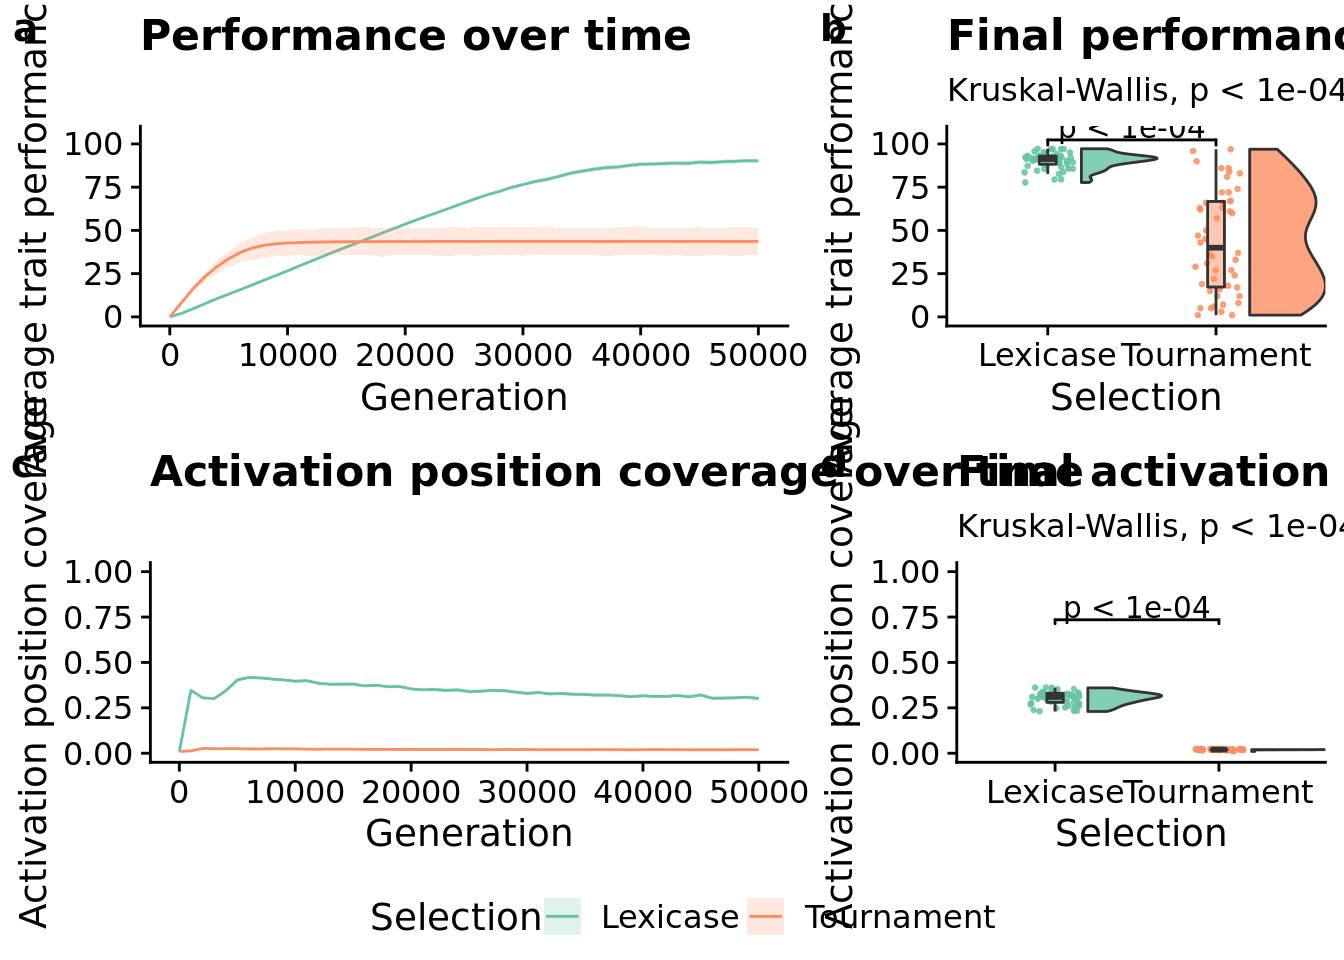
\includegraphics{supplemental-material_files/figure-latex/unnamed-chunk-14-1.pdf}

\hypertarget{diagnostic-cardinality}{%
\chapter{Diagnostic cardinality}\label{diagnostic-cardinality}}

\hypertarget{overview-1}{%
\section{Overview}\label{overview-1}}

\begin{Shaded}
\begin{Highlighting}[]
\CommentTok{# Relative location of data.}
\NormalTok{working_directory <-}
\StringTok{  "experiments/2021-05-27-cardinality/analysis/"}
\CommentTok{# working_directory <- "./"}

\CommentTok{# Settings for visualization}
\NormalTok{cb_palette <-}\StringTok{ "Set2"}
\CommentTok{# Create directory to dump plots}
\KeywordTok{dir.create}\NormalTok{(}\KeywordTok{paste0}\NormalTok{(working_directory, }\StringTok{"imgs"}\NormalTok{), }\DataTypeTok{showWarnings=}\OtherTok{FALSE}\NormalTok{)}
\end{Highlighting}
\end{Shaded}

\hypertarget{analysis-dependencies-1}{%
\section{Analysis dependencies}\label{analysis-dependencies-1}}

\begin{Shaded}
\begin{Highlighting}[]
\KeywordTok{library}\NormalTok{(ggplot2)}
\KeywordTok{library}\NormalTok{(tidyverse)}
\KeywordTok{library}\NormalTok{(knitr)}
\KeywordTok{library}\NormalTok{(cowplot)}
\KeywordTok{library}\NormalTok{(viridis)}
\KeywordTok{library}\NormalTok{(RColorBrewer)}
\KeywordTok{library}\NormalTok{(rstatix)}
\KeywordTok{library}\NormalTok{(ggsignif)}
\KeywordTok{library}\NormalTok{(Hmisc)}
\KeywordTok{source}\NormalTok{(}\StringTok{"https://gist.githubusercontent.com/benmarwick/2a1bb0133ff568cbe28d/raw/fb53bd97121f7f9ce947837ef1a4c65a73bffb3f/geom_flat_violin.R"}\NormalTok{)}
\end{Highlighting}
\end{Shaded}

These analyses were conducted in the following computing environment:

\begin{Shaded}
\begin{Highlighting}[]
\KeywordTok{print}\NormalTok{(version)}
\end{Highlighting}
\end{Shaded}

\begin{verbatim}
##                _                           
## platform       x86_64-pc-linux-gnu         
## arch           x86_64                      
## os             linux-gnu                   
## system         x86_64, linux-gnu           
## status                                     
## major          4                           
## minor          1.0                         
## year           2021                        
## month          05                          
## day            18                          
## svn rev        80317                       
## language       R                           
## version.string R version 4.1.0 (2021-05-18)
## nickname       Camp Pontanezen
\end{verbatim}

\hypertarget{setup-1}{%
\section{Setup}\label{setup-1}}

\begin{Shaded}
\begin{Highlighting}[]
\NormalTok{data_loc <-}\StringTok{ }\KeywordTok{paste0}\NormalTok{(}
\NormalTok{  working_directory,}
  \StringTok{"data/timeseries-res-1000g.csv"}
\NormalTok{)}
\NormalTok{data <-}\StringTok{ }\KeywordTok{read.csv}\NormalTok{(}
\NormalTok{  data_loc,}
  \DataTypeTok{na.strings=}\StringTok{"NONE"}
\NormalTok{)}

\NormalTok{data}\OperatorTok{$}\NormalTok{cardinality <-}\StringTok{ }\KeywordTok{as.factor}\NormalTok{(}
\NormalTok{  data}\OperatorTok{$}\NormalTok{OBJECTIVE_CNT}
\NormalTok{)}
\NormalTok{data}\OperatorTok{$}\NormalTok{selection_name <-}\StringTok{ }\KeywordTok{as.factor}\NormalTok{(}
\NormalTok{  data}\OperatorTok{$}\NormalTok{selection_name}
\NormalTok{)}

\NormalTok{data}\OperatorTok{$}\NormalTok{elite_trait_avg <-}
\StringTok{  }\NormalTok{data}\OperatorTok{$}\NormalTok{ele_agg_per }\OperatorTok{/}\StringTok{ }\NormalTok{data}\OperatorTok{$}\NormalTok{OBJECTIVE_CNT}

\NormalTok{data}\OperatorTok{$}\NormalTok{unique_start_positions_coverage <-}
\StringTok{  }\NormalTok{data}\OperatorTok{$}\NormalTok{uni_str_pos }\OperatorTok{/}\StringTok{ }\NormalTok{data}\OperatorTok{$}\NormalTok{OBJECTIVE_CNT}

\NormalTok{final_data <-}\StringTok{ }\KeywordTok{filter}\NormalTok{(data, gen}\OperatorTok{==}\KeywordTok{max}\NormalTok{(data}\OperatorTok{$}\NormalTok{gen))}

\CommentTok{# Labeler for stats annotations}
\NormalTok{p_label <-}\StringTok{ }\ControlFlowTok{function}\NormalTok{(p_value) \{}
\NormalTok{  threshold =}\StringTok{ }\FloatTok{0.0001}
  \ControlFlowTok{if}\NormalTok{ (p_value }\OperatorTok{<}\StringTok{ }\NormalTok{threshold) \{}
    \KeywordTok{return}\NormalTok{(}\KeywordTok{paste0}\NormalTok{(}\StringTok{"p < "}\NormalTok{, threshold))}
\NormalTok{  \} }\ControlFlowTok{else}\NormalTok{ \{}
    \KeywordTok{return}\NormalTok{(}\KeywordTok{paste0}\NormalTok{(}\StringTok{"p = "}\NormalTok{, p_value))}
\NormalTok{  \}}
\NormalTok{\}}

\CommentTok{# Significance threshold}
\NormalTok{alpha <-}\StringTok{ }\FloatTok{0.05}

\CommentTok{####### misc #######}
\CommentTok{# Configure our default graphing theme}
\KeywordTok{theme_set}\NormalTok{(}\KeywordTok{theme_cowplot}\NormalTok{())}
\end{Highlighting}
\end{Shaded}

\hypertarget{exploration-diagnostic-performance-1}{%
\section{Exploration diagnostic performance}\label{exploration-diagnostic-performance-1}}

First, we look at performance over time.
Specifically, we look at the normalized aggregage score of the most performant individuals over time.
To control for different cardinalities having different maximum scores, we normalized performances (by dividing by cardinality) to values between 0 and 100.

\begin{Shaded}
\begin{Highlighting}[]
\NormalTok{elite_trait_ave_fit <-}\StringTok{ }\KeywordTok{ggplot}\NormalTok{(}
\NormalTok{    data,}
    \KeywordTok{aes}\NormalTok{(}
      \DataTypeTok{x=}\NormalTok{gen,}
      \DataTypeTok{y=}\NormalTok{elite_trait_avg,}
      \DataTypeTok{color=}\NormalTok{cardinality,}
      \DataTypeTok{fill=}\NormalTok{cardinality}
\NormalTok{    )}
\NormalTok{  ) }\OperatorTok{+}
\StringTok{  }\KeywordTok{stat_summary}\NormalTok{(}\DataTypeTok{geom=}\StringTok{"line"}\NormalTok{, }\DataTypeTok{fun=}\NormalTok{mean) }\OperatorTok{+}
\StringTok{  }\KeywordTok{stat_summary}\NormalTok{(}
    \DataTypeTok{geom=}\StringTok{"ribbon"}\NormalTok{,}
    \DataTypeTok{fun.data=}\StringTok{"mean_cl_boot"}\NormalTok{,}
    \DataTypeTok{fun.args=}\KeywordTok{list}\NormalTok{(}\DataTypeTok{conf.int=}\FloatTok{0.95}\NormalTok{),}
    \DataTypeTok{alpha=}\FloatTok{0.2}\NormalTok{,}
    \DataTypeTok{linetype=}\DecValTok{0}
\NormalTok{  ) }\OperatorTok{+}
\StringTok{  }\KeywordTok{scale_y_continuous}\NormalTok{(}
    \DataTypeTok{name=}\StringTok{"Average trait performance"}\NormalTok{,}
    \DataTypeTok{limits=}\KeywordTok{c}\NormalTok{(}\DecValTok{0}\NormalTok{, }\DecValTok{100}\NormalTok{)}
\NormalTok{  ) }\OperatorTok{+}
\StringTok{  }\KeywordTok{scale_x_continuous}\NormalTok{(}
    \DataTypeTok{name=}\StringTok{"Generation"}
\NormalTok{  ) }\OperatorTok{+}
\StringTok{  }\KeywordTok{scale_fill_brewer}\NormalTok{(}
    \DataTypeTok{name=}\StringTok{"Cardinaltiy"}\NormalTok{,}
    \DataTypeTok{palette=}\NormalTok{cb_palette}
\NormalTok{  ) }\OperatorTok{+}
\StringTok{  }\KeywordTok{scale_color_brewer}\NormalTok{(}
    \DataTypeTok{name=}\StringTok{"Cardinaltiy"}\NormalTok{,}
    \DataTypeTok{palette=}\NormalTok{cb_palette}
\NormalTok{  )}
\NormalTok{elite_trait_ave_fit}
\end{Highlighting}
\end{Shaded}

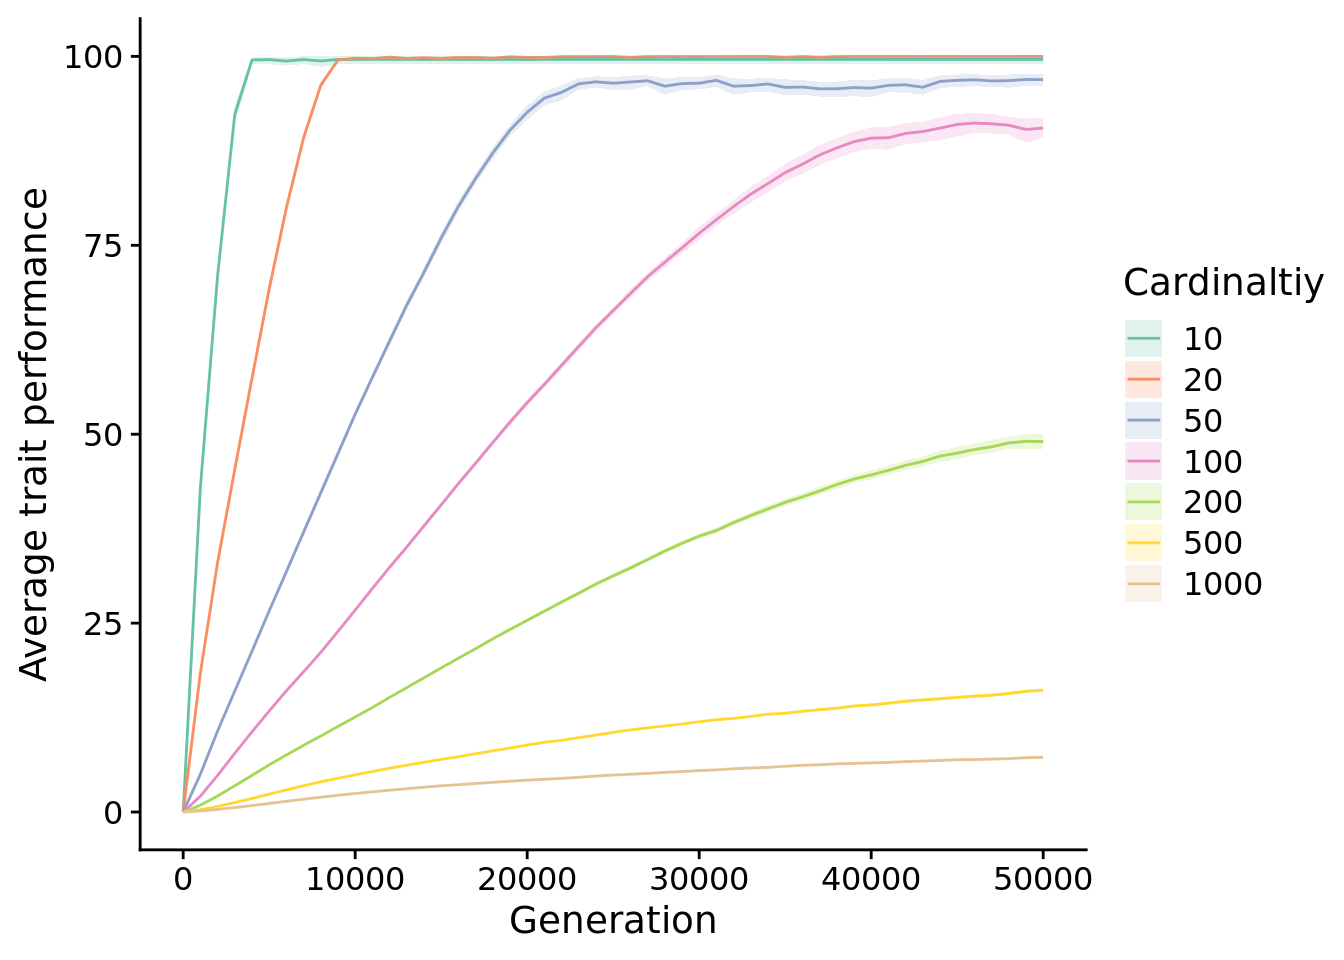
\includegraphics{supplemental-material_files/figure-latex/unnamed-chunk-19-1.pdf}

\hypertarget{final-performance-1}{%
\subsection{Final performance}\label{final-performance-1}}

Next, we look only at the final performances of each treatment

\begin{Shaded}
\begin{Highlighting}[]
\CommentTok{# Compute manual labels for geom_signif}
\NormalTok{stat.test <-}\StringTok{ }\NormalTok{final_data }\OperatorTok
\StringTok{  }\KeywordTok{wilcox_test}\NormalTok{(elite_trait_avg }\OperatorTok{~}\StringTok{ }\NormalTok{cardinality) }\OperatorTok
\StringTok{  }\KeywordTok{adjust_pvalue}\NormalTok{(}\DataTypeTok{method =} \StringTok{"bonferroni"}\NormalTok{) }\OperatorTok
\StringTok{  }\KeywordTok{add_significance}\NormalTok{() }\OperatorTok
\StringTok{  }\KeywordTok{add_xy_position}\NormalTok{(}\DataTypeTok{x=}\StringTok{"cardinality"}\NormalTok{,}\DataTypeTok{step.increase=}\DecValTok{1}\NormalTok{)}
\NormalTok{stat.test}\OperatorTok{$}\NormalTok{manual_position <-}\StringTok{ }\NormalTok{stat.test}\OperatorTok{$}\NormalTok{y.position }\OperatorTok{*}\StringTok{ }\FloatTok{1.05}
\NormalTok{stat.test}\OperatorTok{$}\NormalTok{label <-}\StringTok{ }\KeywordTok{mapply}\NormalTok{(p_label,stat.test}\OperatorTok{$}\NormalTok{p.adj)}
\end{Highlighting}
\end{Shaded}

\begin{Shaded}
\begin{Highlighting}[]
\NormalTok{elite_trait_ave_fit_final <-}\StringTok{ }\KeywordTok{ggplot}\NormalTok{(}
\NormalTok{    final_data,}
    \KeywordTok{aes}\NormalTok{(}\DataTypeTok{x=}\NormalTok{cardinality, }\DataTypeTok{y=}\NormalTok{elite_trait_avg, }\DataTypeTok{fill=}\NormalTok{cardinality)}
\NormalTok{  ) }\OperatorTok{+}
\StringTok{  }\KeywordTok{geom_flat_violin}\NormalTok{(}
    \DataTypeTok{position =} \KeywordTok{position_nudge}\NormalTok{(}\DataTypeTok{x =} \FloatTok{.2}\NormalTok{, }\DataTypeTok{y =} \DecValTok{0}\NormalTok{),}
    \DataTypeTok{alpha =} \FloatTok{.8}\NormalTok{,}
    \DataTypeTok{scale=}\StringTok{"width"}
\NormalTok{  ) }\OperatorTok{+}
\StringTok{  }\KeywordTok{geom_point}\NormalTok{(}
    \DataTypeTok{mapping=}\KeywordTok{aes}\NormalTok{(}\DataTypeTok{color=}\NormalTok{cardinality),}
    \DataTypeTok{position =} \KeywordTok{position_jitter}\NormalTok{(}\DataTypeTok{width =} \FloatTok{.15}\NormalTok{),}
    \DataTypeTok{size =} \FloatTok{.5}\NormalTok{,}
    \DataTypeTok{alpha =} \FloatTok{0.8}
\NormalTok{  ) }\OperatorTok{+}
\StringTok{  }\KeywordTok{geom_boxplot}\NormalTok{(}
    \DataTypeTok{width =} \FloatTok{.1}\NormalTok{,}
    \DataTypeTok{outlier.shape =} \OtherTok{NA}\NormalTok{,}
    \DataTypeTok{alpha =} \FloatTok{0.5}
\NormalTok{  ) }\OperatorTok{+}
\StringTok{  }\KeywordTok{scale_y_continuous}\NormalTok{(}
    \DataTypeTok{name=}\StringTok{"Average trait performance"}\NormalTok{,}
    \DataTypeTok{limits=}\KeywordTok{c}\NormalTok{(}\DecValTok{0}\NormalTok{, }\DecValTok{100}\NormalTok{)}
\NormalTok{  ) }\OperatorTok{+}
\StringTok{  }\KeywordTok{scale_x_discrete}\NormalTok{(}
    \DataTypeTok{name=}\StringTok{"Cardinality"}
\NormalTok{  ) }\OperatorTok{+}
\StringTok{  }\KeywordTok{scale_fill_brewer}\NormalTok{(}
    \DataTypeTok{name=}\StringTok{"Cardinaltiy"}\NormalTok{,}
    \DataTypeTok{palette=}\NormalTok{cb_palette}
\NormalTok{  ) }\OperatorTok{+}
\StringTok{  }\KeywordTok{scale_color_brewer}\NormalTok{(}
    \DataTypeTok{name=}\StringTok{"Cardinaltiy"}\NormalTok{,}
    \DataTypeTok{palette=}\NormalTok{cb_palette}
\NormalTok{  ) }\OperatorTok{+}
\StringTok{  }\KeywordTok{theme}\NormalTok{(}
    \DataTypeTok{legend.position=}\StringTok{"none"}
\NormalTok{  )}
\NormalTok{elite_trait_ave_fit_final}
\end{Highlighting}
\end{Shaded}

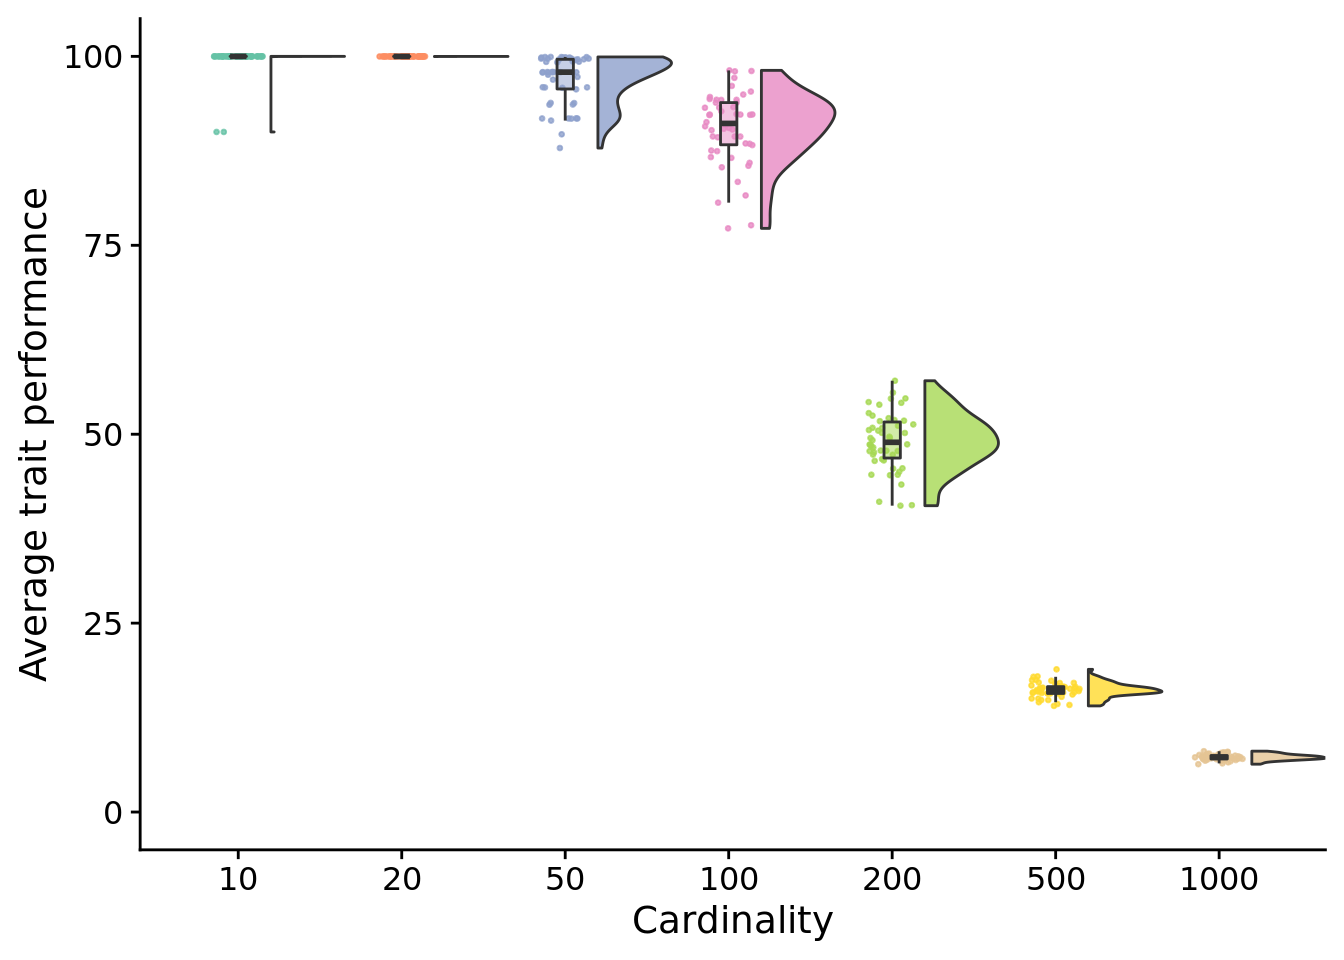
\includegraphics{supplemental-material_files/figure-latex/unnamed-chunk-21-1.pdf}

\begin{tabular}{l|l|l|r|r|r|r|r|l|r|l|r|r|r|l}
\hline
.y. & group1 & group2 & n1 & n2 & statistic & p & p.adj & p.adj.signif & y.position & groups & xmin & xmax & manual\_position & label\\
\hline
elite\_trait\_avg & 10 & 20 & 50 & 50 & 2399 & 0 & 0 & **** & 191.9440 & 10, 20 & 1 & 2 & 201.5412 & p < 1e-04\\
\hline
elite\_trait\_avg & 10 & 50 & 50 & 50 & 2404 & 0 & 0 & **** & 288.4852 & 10, 50 & 1 & 3 & 302.9095 & p < 1e-04\\
\hline
elite\_trait\_avg & 10 & 100 & 50 & 50 & 2438 & 0 & 0 & **** & 385.0264 & 10 , 100 & 1 & 4 & 404.2777 & p < 1e-04\\
\hline
elite\_trait\_avg & 10 & 200 & 50 & 50 & 2500 & 0 & 0 & **** & 481.5676 & 10 , 200 & 1 & 5 & 505.6460 & p < 1e-04\\
\hline
elite\_trait\_avg & 10 & 500 & 50 & 50 & 2500 & 0 & 0 & **** & 578.1088 & 10 , 500 & 1 & 6 & 607.0142 & p < 1e-04\\
\hline
elite\_trait\_avg & 10 & 1000 & 50 & 50 & 2500 & 0 & 0 & **** & 674.6500 & 10  , 1000 & 1 & 7 & 708.3825 & p < 1e-04\\
\hline
elite\_trait\_avg & 20 & 50 & 50 & 50 & 2500 & 0 & 0 & **** & 771.1912 & 20, 50 & 2 & 3 & 809.7508 & p < 1e-04\\
\hline
elite\_trait\_avg & 20 & 100 & 50 & 50 & 2500 & 0 & 0 & **** & 867.7324 & 20 , 100 & 2 & 4 & 911.1190 & p < 1e-04\\
\hline
elite\_trait\_avg & 20 & 200 & 50 & 50 & 2500 & 0 & 0 & **** & 964.2736 & 20 , 200 & 2 & 5 & 1012.4873 & p < 1e-04\\
\hline
elite\_trait\_avg & 20 & 500 & 50 & 50 & 2500 & 0 & 0 & **** & 1060.8148 & 20 , 500 & 2 & 6 & 1113.8555 & p < 1e-04\\
\hline
elite\_trait\_avg & 20 & 1000 & 50 & 50 & 2500 & 0 & 0 & **** & 1157.3560 & 20  , 1000 & 2 & 7 & 1215.2238 & p < 1e-04\\
\hline
elite\_trait\_avg & 50 & 100 & 50 & 50 & 2166 & 0 & 0 & **** & 1253.8972 & 50 , 100 & 3 & 4 & 1316.5921 & p < 1e-04\\
\hline
elite\_trait\_avg & 50 & 200 & 50 & 50 & 2500 & 0 & 0 & **** & 1350.4384 & 50 , 200 & 3 & 5 & 1417.9603 & p < 1e-04\\
\hline
elite\_trait\_avg & 50 & 500 & 50 & 50 & 2500 & 0 & 0 & **** & 1446.9796 & 50 , 500 & 3 & 6 & 1519.3286 & p < 1e-04\\
\hline
elite\_trait\_avg & 50 & 1000 & 50 & 50 & 2500 & 0 & 0 & **** & 1543.5208 & 50  , 1000 & 3 & 7 & 1620.6968 & p < 1e-04\\
\hline
elite\_trait\_avg & 100 & 200 & 50 & 50 & 2500 & 0 & 0 & **** & 1640.0620 & 100, 200 & 4 & 5 & 1722.0651 & p < 1e-04\\
\hline
elite\_trait\_avg & 100 & 500 & 50 & 50 & 2500 & 0 & 0 & **** & 1736.6032 & 100, 500 & 4 & 6 & 1823.4334 & p < 1e-04\\
\hline
elite\_trait\_avg & 100 & 1000 & 50 & 50 & 2500 & 0 & 0 & **** & 1833.1444 & 100 , 1000 & 4 & 7 & 1924.8016 & p < 1e-04\\
\hline
elite\_trait\_avg & 200 & 500 & 50 & 50 & 2500 & 0 & 0 & **** & 1929.6856 & 200, 500 & 5 & 6 & 2026.1699 & p < 1e-04\\
\hline
elite\_trait\_avg & 200 & 1000 & 50 & 50 & 2500 & 0 & 0 & **** & 2026.2268 & 200 , 1000 & 5 & 7 & 2127.5381 & p < 1e-04\\
\hline
elite\_trait\_avg & 500 & 1000 & 50 & 50 & 2500 & 0 & 0 & **** & 2122.7680 & 500 , 1000 & 6 & 7 & 2228.9064 & p < 1e-04\\
\hline
\end{tabular}

\hypertarget{unique-starting-positions-1}{%
\section{Unique starting positions}\label{unique-starting-positions-1}}

Next, we analyze the number of unique starting position maintained by populations.

\begin{Shaded}
\begin{Highlighting}[]
\KeywordTok{ggplot}\NormalTok{(data, }\KeywordTok{aes}\NormalTok{(}\DataTypeTok{x=}\NormalTok{gen, }\DataTypeTok{y=}\NormalTok{uni_str_pos, }\DataTypeTok{color=}\NormalTok{cardinality)) }\OperatorTok{+}
\StringTok{  }\KeywordTok{stat_summary}\NormalTok{(}\DataTypeTok{geom=}\StringTok{"line"}\NormalTok{, }\DataTypeTok{fun=}\NormalTok{mean) }\OperatorTok{+}
\StringTok{  }\KeywordTok{stat_summary}\NormalTok{(}
    \DataTypeTok{geom=}\StringTok{"ribbon"}\NormalTok{,}
    \DataTypeTok{fun.data=}\StringTok{"mean_cl_boot"}\NormalTok{,}
    \DataTypeTok{fun.args=}\KeywordTok{list}\NormalTok{(}\DataTypeTok{conf.int=}\FloatTok{0.95}\NormalTok{),}
    \DataTypeTok{alpha=}\FloatTok{0.2}\NormalTok{,}
    \DataTypeTok{linetype=}\DecValTok{0}
\NormalTok{  ) }\OperatorTok{+}
\StringTok{  }\KeywordTok{scale_y_continuous}\NormalTok{(}
    \DataTypeTok{name=}\StringTok{"Unique activation positions (population)"}\NormalTok{,}
\NormalTok{  ) }\OperatorTok{+}
\StringTok{  }\KeywordTok{scale_x_continuous}\NormalTok{(}
    \DataTypeTok{name=}\StringTok{"Generation"}
\NormalTok{  )}
\end{Highlighting}
\end{Shaded}

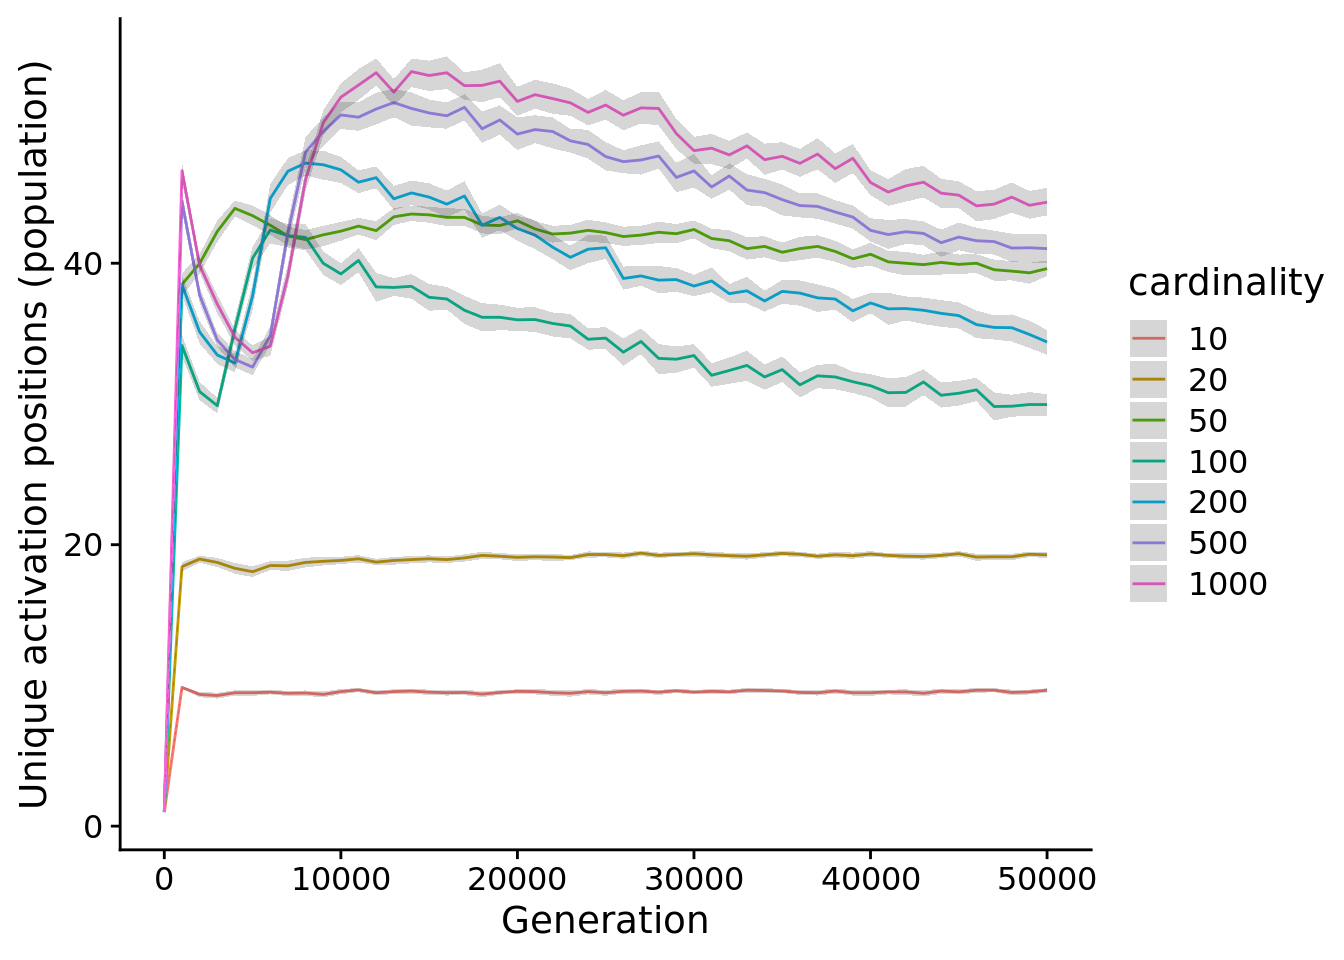
\includegraphics{supplemental-material_files/figure-latex/unnamed-chunk-23-1.pdf}

Different cardinalities have numbers of possible starting positions, so next, we look at the proportion of starting positions (out of all possible) maintained by populations.

\begin{Shaded}
\begin{Highlighting}[]
\NormalTok{unique_start_positions_coverage_fig <-}\StringTok{ }\KeywordTok{ggplot}\NormalTok{(}
\NormalTok{    data,}
    \KeywordTok{aes}\NormalTok{(}
      \DataTypeTok{x=}\NormalTok{gen,}
      \DataTypeTok{y=}\NormalTok{unique_start_positions_coverage,}
      \DataTypeTok{color=}\NormalTok{cardinality,}
      \DataTypeTok{fill=}\NormalTok{cardinality}
\NormalTok{    )}
\NormalTok{  ) }\OperatorTok{+}
\StringTok{  }\KeywordTok{stat_summary}\NormalTok{(}\DataTypeTok{geom=}\StringTok{"line"}\NormalTok{, }\DataTypeTok{fun=}\NormalTok{mean) }\OperatorTok{+}
\StringTok{  }\KeywordTok{stat_summary}\NormalTok{(}
    \DataTypeTok{geom=}\StringTok{"ribbon"}\NormalTok{,}
    \DataTypeTok{fun.data=}\StringTok{"mean_cl_boot"}\NormalTok{,}
    \DataTypeTok{fun.args=}\KeywordTok{list}\NormalTok{(}\DataTypeTok{conf.int=}\FloatTok{0.95}\NormalTok{),}
    \DataTypeTok{alpha=}\FloatTok{0.2}\NormalTok{,}
    \DataTypeTok{linetype=}\DecValTok{0}
\NormalTok{  ) }\OperatorTok{+}
\StringTok{  }\KeywordTok{scale_y_continuous}\NormalTok{(}
    \DataTypeTok{name=}\StringTok{"Activation position coverage"}\NormalTok{,}
    \DataTypeTok{limits=}\KeywordTok{c}\NormalTok{(}\FloatTok{0.0}\NormalTok{, }\FloatTok{1.05}\NormalTok{)}
\NormalTok{  ) }\OperatorTok{+}
\StringTok{  }\KeywordTok{scale_x_continuous}\NormalTok{(}
    \DataTypeTok{name=}\StringTok{"Generation"}
\NormalTok{  ) }\OperatorTok{+}
\StringTok{  }\KeywordTok{scale_fill_brewer}\NormalTok{(}
    \DataTypeTok{name=}\StringTok{"Cardinaltiy"}\NormalTok{,}
    \DataTypeTok{palette=}\NormalTok{cb_palette}
\NormalTok{  ) }\OperatorTok{+}
\StringTok{  }\KeywordTok{scale_color_brewer}\NormalTok{(}
    \DataTypeTok{name=}\StringTok{"Cardinaltiy"}\NormalTok{,}
    \DataTypeTok{palette=}\NormalTok{cb_palette}
\NormalTok{  )}
\NormalTok{unique_start_positions_coverage_fig}
\end{Highlighting}
\end{Shaded}

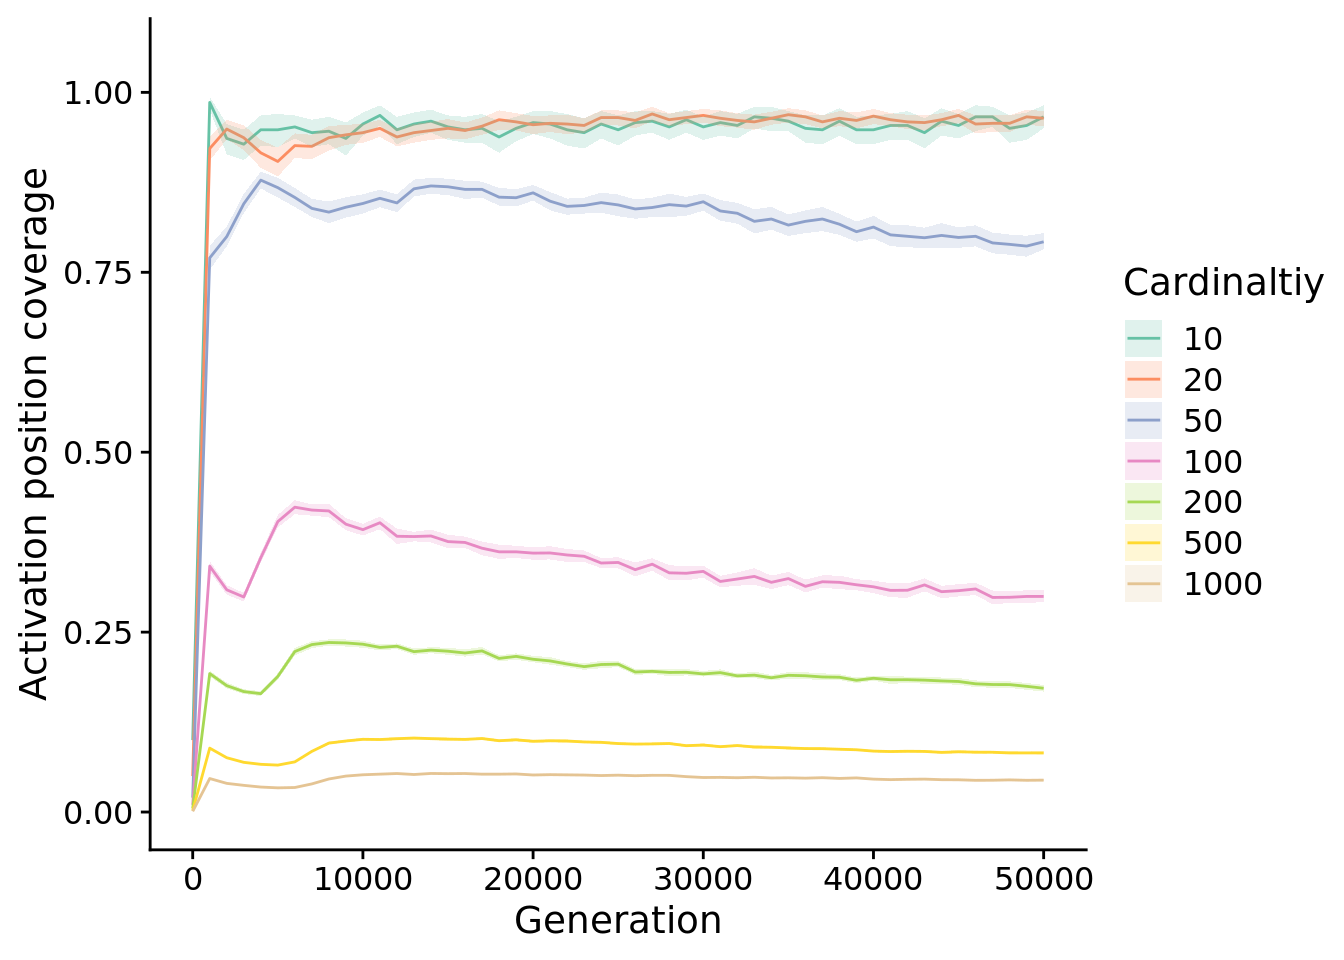
\includegraphics{supplemental-material_files/figure-latex/unnamed-chunk-24-1.pdf}

\hypertarget{final-starting-position-coverage-1}{%
\subsection{Final starting position coverage}\label{final-starting-position-coverage-1}}

\begin{Shaded}
\begin{Highlighting}[]
\CommentTok{# Compute manual labels for geom_signif}
\NormalTok{stat.test <-}\StringTok{ }\NormalTok{final_data }\OperatorTok
\StringTok{  }\KeywordTok{wilcox_test}\NormalTok{(unique_start_positions_coverage }\OperatorTok{~}\StringTok{ }\NormalTok{cardinality) }\OperatorTok
\StringTok{  }\KeywordTok{adjust_pvalue}\NormalTok{(}\DataTypeTok{method =} \StringTok{"bonferroni"}\NormalTok{) }\OperatorTok
\StringTok{  }\KeywordTok{add_significance}\NormalTok{() }\OperatorTok
\StringTok{  }\KeywordTok{add_xy_position}\NormalTok{(}\DataTypeTok{x=}\StringTok{"cardinality"}\NormalTok{,}\DataTypeTok{step.increase=}\DecValTok{1}\NormalTok{)}
\NormalTok{stat.test}\OperatorTok{$}\NormalTok{manual_position <-}\StringTok{ }\NormalTok{stat.test}\OperatorTok{$}\NormalTok{y.position }\OperatorTok{*}\StringTok{ }\FloatTok{1.05}
\NormalTok{stat.test}\OperatorTok{$}\NormalTok{label <-}\StringTok{ }\KeywordTok{mapply}\NormalTok{(p_label,stat.test}\OperatorTok{$}\NormalTok{p.adj)}
\end{Highlighting}
\end{Shaded}

\begin{Shaded}
\begin{Highlighting}[]
\NormalTok{final_unique_start_positions_coverage_fig <-}\StringTok{ }\KeywordTok{ggplot}\NormalTok{(}
\NormalTok{    final_data,}
    \KeywordTok{aes}\NormalTok{(}
      \DataTypeTok{x=}\NormalTok{cardinality,}
      \DataTypeTok{y=}\NormalTok{unique_start_positions_coverage,}
      \DataTypeTok{fill=}\NormalTok{cardinality}
\NormalTok{    )}
\NormalTok{  ) }\OperatorTok{+}
\StringTok{  }\KeywordTok{geom_flat_violin}\NormalTok{(}
    \DataTypeTok{position =} \KeywordTok{position_nudge}\NormalTok{(}\DataTypeTok{x =} \FloatTok{.2}\NormalTok{, }\DataTypeTok{y =} \DecValTok{0}\NormalTok{),}
    \DataTypeTok{alpha =} \FloatTok{.8}\NormalTok{,}
    \DataTypeTok{scale=}\StringTok{"width"}
\NormalTok{  ) }\OperatorTok{+}
\StringTok{  }\KeywordTok{geom_point}\NormalTok{(}
    \DataTypeTok{mapping=}\KeywordTok{aes}\NormalTok{(}\DataTypeTok{color=}\NormalTok{cardinality),}
    \DataTypeTok{position =} \KeywordTok{position_jitter}\NormalTok{(}\DataTypeTok{width =} \FloatTok{.15}\NormalTok{),}
    \DataTypeTok{size =} \FloatTok{.5}\NormalTok{,}
    \DataTypeTok{alpha =} \FloatTok{0.8}
\NormalTok{  ) }\OperatorTok{+}
\StringTok{  }\KeywordTok{geom_boxplot}\NormalTok{(}
    \DataTypeTok{width =} \FloatTok{.1}\NormalTok{,}
    \DataTypeTok{outlier.shape =} \OtherTok{NA}\NormalTok{,}
    \DataTypeTok{alpha =} \FloatTok{0.5}
\NormalTok{  ) }\OperatorTok{+}
\StringTok{  }\KeywordTok{scale_y_continuous}\NormalTok{(}
    \DataTypeTok{name=}\StringTok{"Activation position coverage"}\NormalTok{,}
    \DataTypeTok{limits=}\KeywordTok{c}\NormalTok{(}\DecValTok{0}\NormalTok{, }\FloatTok{1.05}\NormalTok{)}
\NormalTok{  ) }\OperatorTok{+}
\StringTok{  }\KeywordTok{scale_x_discrete}\NormalTok{(}
    \DataTypeTok{name=}\StringTok{"Cardinality"}
\NormalTok{  ) }\OperatorTok{+}
\StringTok{  }\KeywordTok{scale_fill_brewer}\NormalTok{(}
    \DataTypeTok{name=}\StringTok{"Cardinaltiy"}\NormalTok{,}
    \DataTypeTok{palette=}\NormalTok{cb_palette}
\NormalTok{  ) }\OperatorTok{+}
\StringTok{  }\KeywordTok{scale_color_brewer}\NormalTok{(}
    \DataTypeTok{name=}\StringTok{"Cardinaltiy"}\NormalTok{,}
    \DataTypeTok{palette=}\NormalTok{cb_palette}
\NormalTok{  ) }\OperatorTok{+}
\StringTok{  }\KeywordTok{theme}\NormalTok{(}
    \DataTypeTok{legend.position=}\StringTok{"none"}
\NormalTok{  )}
\NormalTok{final_unique_start_positions_coverage_fig}
\end{Highlighting}
\end{Shaded}

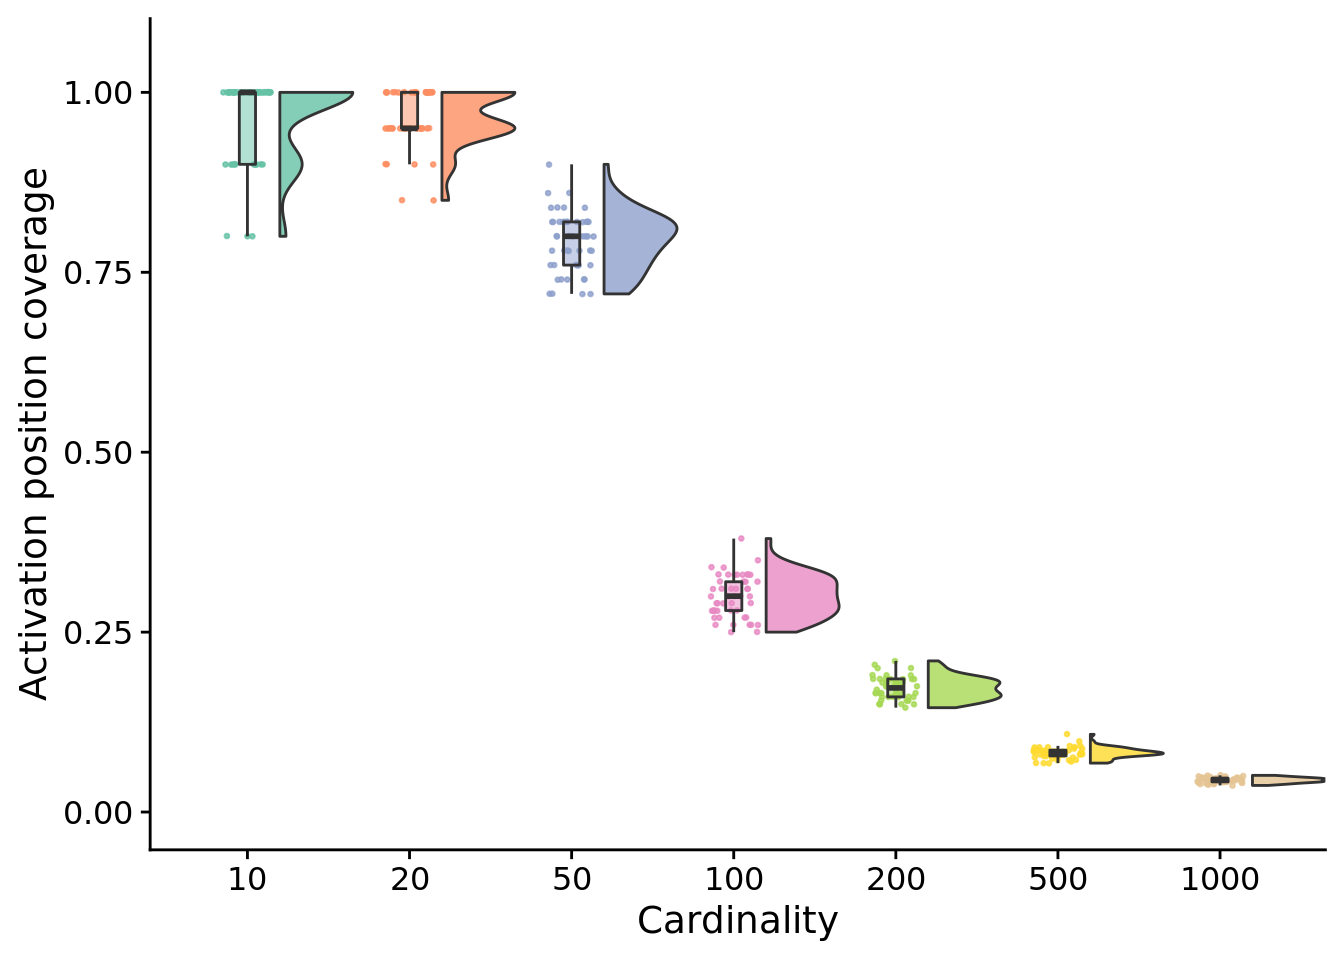
\includegraphics{supplemental-material_files/figure-latex/unnamed-chunk-26-1.pdf}

\begin{tabular}{l|l|l|r|r|r|r|r|l|r|l|r|r|r|l}
\hline
.y. & group1 & group2 & n1 & n2 & statistic & p & p.adj & p.adj.signif & y.position & groups & xmin & xmax & manual\_position & label\\
\hline
unique\_start\_positions\_coverage & 10 & 20 & 50 & 50 & 1448 & 0.126 & 1 & ns & 1.94900 & 10, 20 & 1 & 2 & 2.046450 & p = 1\\
\hline
unique\_start\_positions\_coverage & 10 & 50 & 50 & 50 & 2424 & 0.000 & 0 & **** & 2.94545 & 10, 50 & 1 & 3 & 3.092722 & p < 1e-04\\
\hline
unique\_start\_positions\_coverage & 10 & 100 & 50 & 50 & 2500 & 0.000 & 0 & **** & 3.94190 & 10 , 100 & 1 & 4 & 4.138995 & p < 1e-04\\
\hline
unique\_start\_positions\_coverage & 10 & 200 & 50 & 50 & 2500 & 0.000 & 0 & **** & 4.93835 & 10 , 200 & 1 & 5 & 5.185268 & p < 1e-04\\
\hline
unique\_start\_positions\_coverage & 10 & 500 & 50 & 50 & 2500 & 0.000 & 0 & **** & 5.93480 & 10 , 500 & 1 & 6 & 6.231540 & p < 1e-04\\
\hline
unique\_start\_positions\_coverage & 10 & 1000 & 50 & 50 & 2500 & 0.000 & 0 & **** & 6.93125 & 10  , 1000 & 1 & 7 & 7.277812 & p < 1e-04\\
\hline
unique\_start\_positions\_coverage & 20 & 50 & 50 & 50 & 2492 & 0.000 & 0 & **** & 7.92770 & 20, 50 & 2 & 3 & 8.324085 & p < 1e-04\\
\hline
unique\_start\_positions\_coverage & 20 & 100 & 50 & 50 & 2500 & 0.000 & 0 & **** & 8.92415 & 20 , 100 & 2 & 4 & 9.370358 & p < 1e-04\\
\hline
unique\_start\_positions\_coverage & 20 & 200 & 50 & 50 & 2500 & 0.000 & 0 & **** & 9.92060 & 20 , 200 & 2 & 5 & 10.416630 & p < 1e-04\\
\hline
unique\_start\_positions\_coverage & 20 & 500 & 50 & 50 & 2500 & 0.000 & 0 & **** & 10.91705 & 20 , 500 & 2 & 6 & 11.462903 & p < 1e-04\\
\hline
unique\_start\_positions\_coverage & 20 & 1000 & 50 & 50 & 2500 & 0.000 & 0 & **** & 11.91350 & 20  , 1000 & 2 & 7 & 12.509175 & p < 1e-04\\
\hline
unique\_start\_positions\_coverage & 50 & 100 & 50 & 50 & 2500 & 0.000 & 0 & **** & 12.90995 & 50 , 100 & 3 & 4 & 13.555447 & p < 1e-04\\
\hline
unique\_start\_positions\_coverage & 50 & 200 & 50 & 50 & 2500 & 0.000 & 0 & **** & 13.90640 & 50 , 200 & 3 & 5 & 14.601720 & p < 1e-04\\
\hline
unique\_start\_positions\_coverage & 50 & 500 & 50 & 50 & 2500 & 0.000 & 0 & **** & 14.90285 & 50 , 500 & 3 & 6 & 15.647993 & p < 1e-04\\
\hline
unique\_start\_positions\_coverage & 50 & 1000 & 50 & 50 & 2500 & 0.000 & 0 & **** & 15.89930 & 50  , 1000 & 3 & 7 & 16.694265 & p < 1e-04\\
\hline
unique\_start\_positions\_coverage & 100 & 200 & 50 & 50 & 2500 & 0.000 & 0 & **** & 16.89575 & 100, 200 & 4 & 5 & 17.740537 & p < 1e-04\\
\hline
unique\_start\_positions\_coverage & 100 & 500 & 50 & 50 & 2500 & 0.000 & 0 & **** & 17.89220 & 100, 500 & 4 & 6 & 18.786810 & p < 1e-04\\
\hline
unique\_start\_positions\_coverage & 100 & 1000 & 50 & 50 & 2500 & 0.000 & 0 & **** & 18.88865 & 100 , 1000 & 4 & 7 & 19.833082 & p < 1e-04\\
\hline
unique\_start\_positions\_coverage & 200 & 500 & 50 & 50 & 2500 & 0.000 & 0 & **** & 19.88510 & 200, 500 & 5 & 6 & 20.879355 & p < 1e-04\\
\hline
unique\_start\_positions\_coverage & 200 & 1000 & 50 & 50 & 2500 & 0.000 & 0 & **** & 20.88155 & 200 , 1000 & 5 & 7 & 21.925628 & p < 1e-04\\
\hline
unique\_start\_positions\_coverage & 500 & 1000 & 50 & 50 & 2500 & 0.000 & 0 & **** & 21.87800 & 500 , 1000 & 6 & 7 & 22.971900 & p < 1e-04\\
\hline
\end{tabular}

\hypertarget{does-activation-position-coverage-predict-performance}{%
\section{Does activation position coverage predict performance?}\label{does-activation-position-coverage-predict-performance}}

\begin{Shaded}
\begin{Highlighting}[]
\KeywordTok{ggplot}\NormalTok{(}
\NormalTok{    final_data,}
    \KeywordTok{aes}\NormalTok{(}
      \DataTypeTok{x=}\NormalTok{unique_start_positions_coverage,}
      \DataTypeTok{y=}\NormalTok{elite_trait_avg,}
      \DataTypeTok{color=}\NormalTok{cardinality}
\NormalTok{    )}
\NormalTok{  ) }\OperatorTok{+}
\StringTok{  }\KeywordTok{geom_point}\NormalTok{() }\OperatorTok{+}
\StringTok{  }\KeywordTok{scale_color_brewer}\NormalTok{(}
    \DataTypeTok{name=}\StringTok{"Cardinaltiy"}\NormalTok{,}
    \DataTypeTok{palette=}\NormalTok{cb_palette}
\NormalTok{  )}
\end{Highlighting}
\end{Shaded}

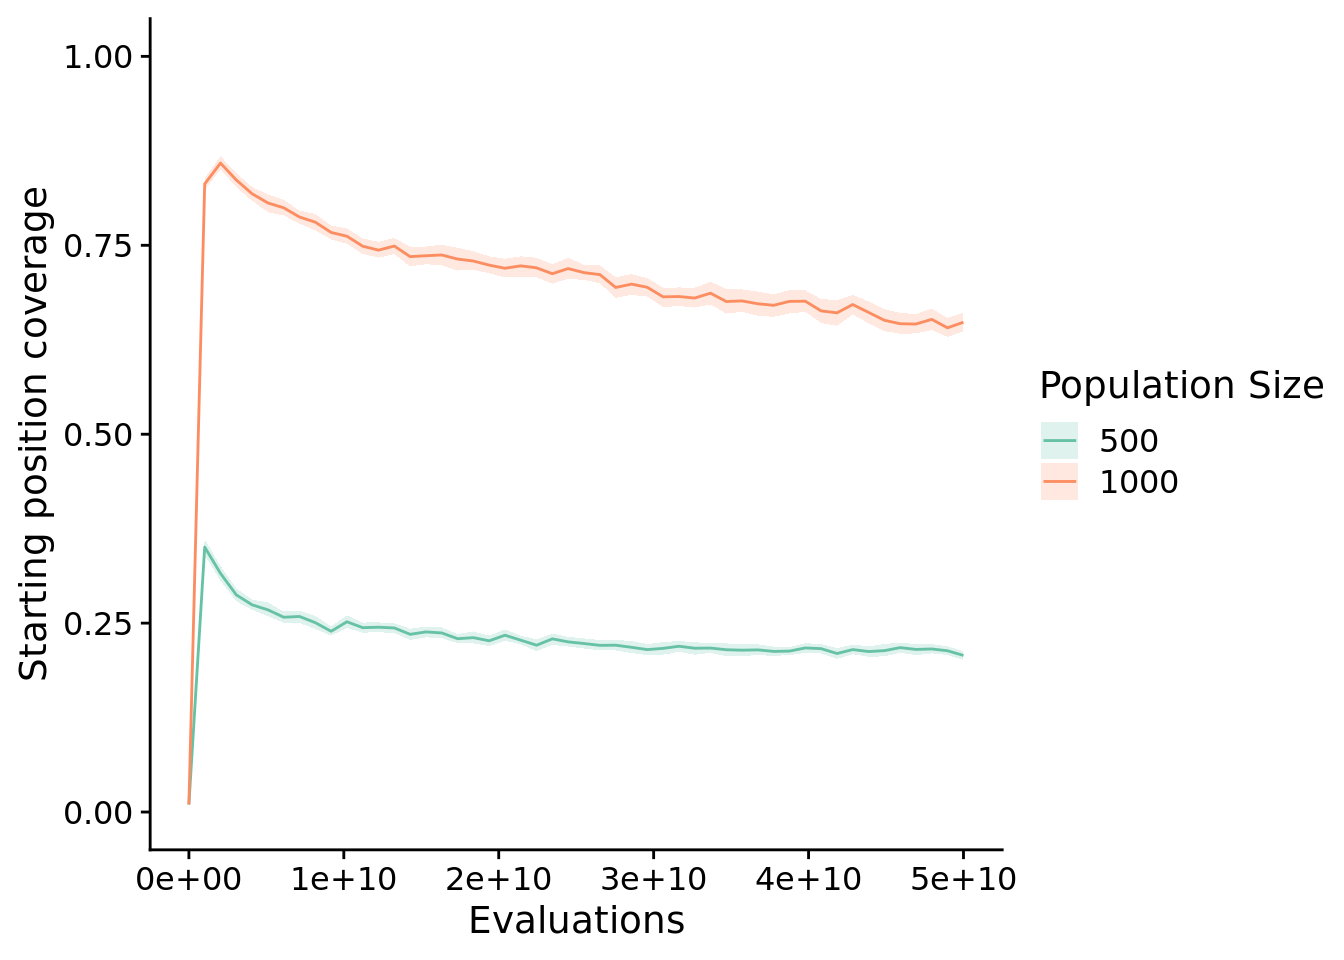
\includegraphics{supplemental-material_files/figure-latex/unnamed-chunk-28-1.pdf}

\begin{Shaded}
\begin{Highlighting}[]
\KeywordTok{cor.test}\NormalTok{(}
  \DataTypeTok{x=}\NormalTok{final_data}\OperatorTok{$}\NormalTok{unique_start_positions_coverage,}
  \DataTypeTok{y=}\NormalTok{final_data}\OperatorTok{$}\NormalTok{elite_trait_avg,}
  \DataTypeTok{method=}\StringTok{"spearman"}\NormalTok{,}
  \DataTypeTok{exact=}\OtherTok{FALSE}
\NormalTok{)}
\end{Highlighting}
\end{Shaded}

\begin{verbatim}
## 
##  Spearman's rank correlation rho
## 
## data:  final_data$unique_start_positions_coverage and final_data$elite_trait_avg
## S = 262488, p-value < 2.2e-16
## alternative hypothesis: true rho is not equal to 0
## sample estimates:
##       rho 
## 0.9632668
\end{verbatim}

\hypertarget{manuscript-figures-1}{%
\section{Manuscript figures}\label{manuscript-figures-1}}

Combine figures for the manuscript.

\begin{Shaded}
\begin{Highlighting}[]
\NormalTok{legend <-}\StringTok{ }\NormalTok{cowplot}\OperatorTok{::}\KeywordTok{get_legend}\NormalTok{(}
\NormalTok{    elite_trait_ave_fit }\OperatorTok{+}
\StringTok{      }\KeywordTok{guides}\NormalTok{(}
        \DataTypeTok{color=}\KeywordTok{guide_legend}\NormalTok{(}\DataTypeTok{nrow=}\DecValTok{1}\NormalTok{),}
        \DataTypeTok{fill=}\KeywordTok{guide_legend}\NormalTok{(}\DataTypeTok{nrow=}\DecValTok{1}\NormalTok{)}
\NormalTok{      ) }\OperatorTok{+}
\StringTok{      }\KeywordTok{theme}\NormalTok{(}
        \DataTypeTok{legend.position =} \StringTok{"bottom"}\NormalTok{,}
        \DataTypeTok{legend.box=}\StringTok{"horizontal"}\NormalTok{,}
        \DataTypeTok{legend.justification=}\StringTok{"center"}
\NormalTok{      )}
\NormalTok{  )}

\NormalTok{grid <-}\StringTok{ }\KeywordTok{plot_grid}\NormalTok{(}
\NormalTok{  elite_trait_ave_fit }\OperatorTok{+}
\StringTok{    }\KeywordTok{ggtitle}\NormalTok{(}\StringTok{"Performance over time"}\NormalTok{) }\OperatorTok{+}
\StringTok{    }\KeywordTok{theme}\NormalTok{(}\DataTypeTok{legend.position=}\StringTok{"none"}\NormalTok{),}
\NormalTok{  elite_trait_ave_fit_final }\OperatorTok{+}
\StringTok{    }\KeywordTok{ggtitle}\NormalTok{(}\StringTok{"Final performance"}\NormalTok{) }\OperatorTok{+}
\StringTok{    }\KeywordTok{theme}\NormalTok{(),}
\NormalTok{  unique_start_positions_coverage_fig }\OperatorTok{+}
\StringTok{    }\KeywordTok{ggtitle}\NormalTok{(}\StringTok{"Activation position coverage over time"}\NormalTok{) }\OperatorTok{+}
\StringTok{    }\KeywordTok{theme}\NormalTok{(}\DataTypeTok{legend.position=}\StringTok{"none"}\NormalTok{),}
\NormalTok{  final_unique_start_positions_coverage_fig }\OperatorTok{+}
\StringTok{    }\KeywordTok{ggtitle}\NormalTok{(}\StringTok{"Final activation position coverage"}\NormalTok{) }\OperatorTok{+}
\StringTok{    }\KeywordTok{theme}\NormalTok{(),}
  \DataTypeTok{nrow=}\DecValTok{2}\NormalTok{,}
  \DataTypeTok{ncol=}\DecValTok{2}\NormalTok{,}
  \DataTypeTok{rel_widths=}\KeywordTok{c}\NormalTok{(}\DecValTok{3}\NormalTok{,}\DecValTok{2}\NormalTok{),}
  \DataTypeTok{labels=}\StringTok{"auto"}
\NormalTok{)}

\NormalTok{grid <-}\StringTok{ }\KeywordTok{plot_grid}\NormalTok{(}
\NormalTok{  grid,}
\NormalTok{  legend,}
  \DataTypeTok{nrow=}\DecValTok{2}\NormalTok{,}
  \DataTypeTok{ncol=}\DecValTok{1}\NormalTok{,}
  \DataTypeTok{rel_heights=}\KeywordTok{c}\NormalTok{(}\DecValTok{1}\NormalTok{, }\FloatTok{0.1}\NormalTok{)}
\NormalTok{)}

\KeywordTok{save_plot}\NormalTok{(}
  \KeywordTok{paste}\NormalTok{(working_directory, }\StringTok{"imgs/cardinality-panel.pdf"}\NormalTok{, }\DataTypeTok{sep=}\StringTok{""}\NormalTok{),}
\NormalTok{  grid,}
  \DataTypeTok{base_width=}\DecValTok{12}\NormalTok{,}
  \DataTypeTok{base_height=}\DecValTok{8}
\NormalTok{)}

\NormalTok{grid}
\end{Highlighting}
\end{Shaded}

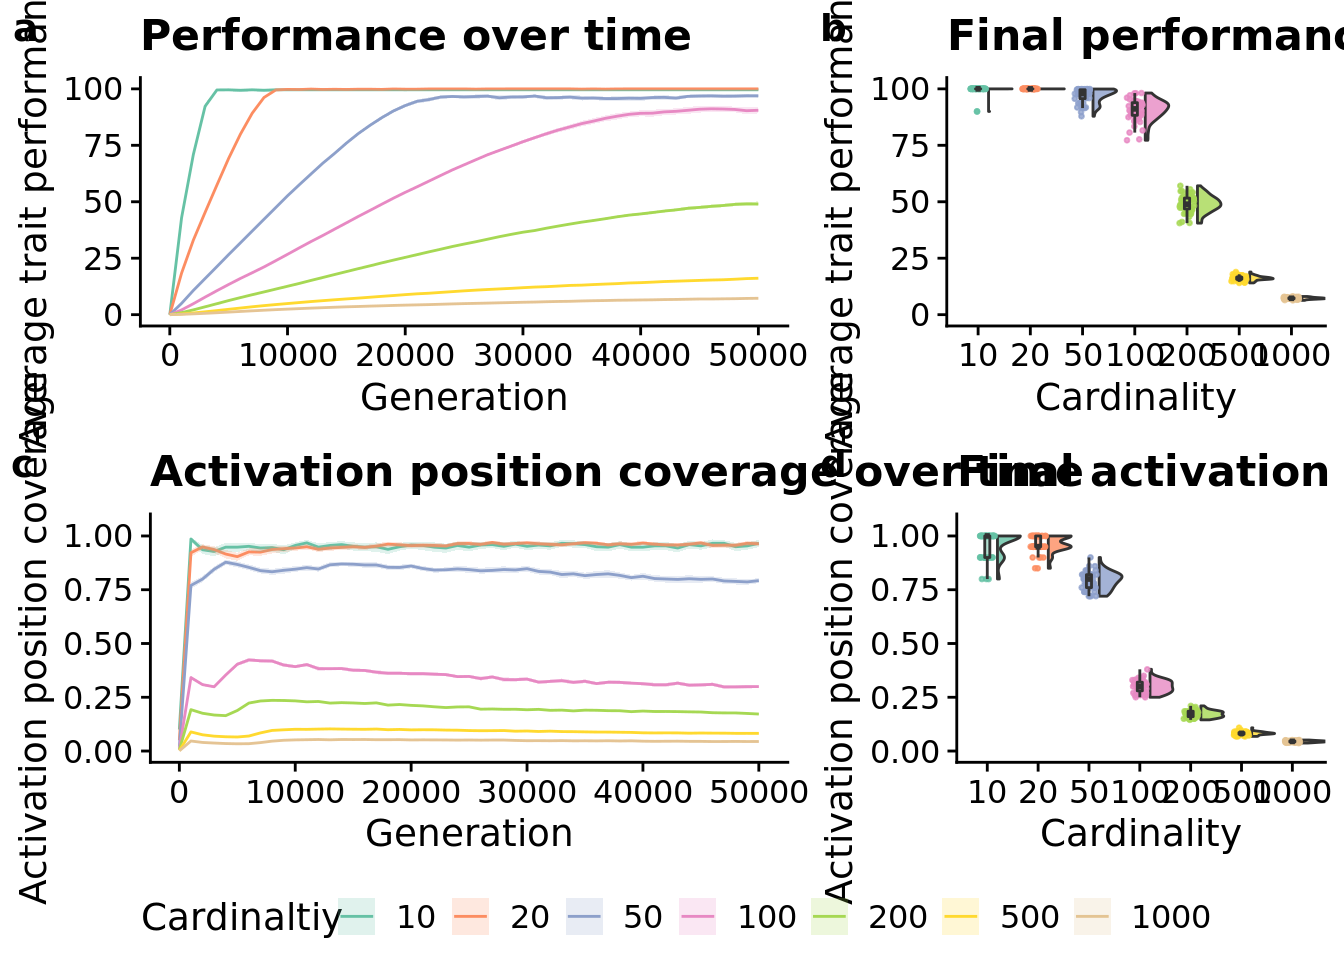
\includegraphics{supplemental-material_files/figure-latex/unnamed-chunk-30-1.pdf}

\hypertarget{increasing-population-size-versus-increasing-generations}{%
\chapter{Increasing population size versus increasing generations}\label{increasing-population-size-versus-increasing-generations}}

\hypertarget{overview-2}{%
\section{Overview}\label{overview-2}}

\begin{Shaded}
\begin{Highlighting}[]
\CommentTok{# Relative location of data.}
\NormalTok{working_directory <-}
\StringTok{  "experiments/2021-06-03-cardinality-pop-size/analysis/"}
\CommentTok{# working_directory <- "./"}

\CommentTok{# Settings for visualization}
\NormalTok{cb_palette <-}\StringTok{ "Set2"}

\CommentTok{# Create directory to dump plots}
\KeywordTok{dir.create}\NormalTok{(}\KeywordTok{paste0}\NormalTok{(working_directory, }\StringTok{"imgs"}\NormalTok{), }\DataTypeTok{showWarnings=}\OtherTok{FALSE}\NormalTok{)}
\end{Highlighting}
\end{Shaded}

\hypertarget{analysis-dependencies-2}{%
\section{Analysis dependencies}\label{analysis-dependencies-2}}

\begin{Shaded}
\begin{Highlighting}[]
\KeywordTok{library}\NormalTok{(ggplot2)}
\KeywordTok{library}\NormalTok{(tidyverse)}
\KeywordTok{library}\NormalTok{(cowplot)}
\KeywordTok{library}\NormalTok{(viridis)}
\KeywordTok{library}\NormalTok{(RColorBrewer)}
\KeywordTok{source}\NormalTok{(}\StringTok{"https://gist.githubusercontent.com/benmarwick/2a1bb0133ff568cbe28d/raw/fb53bd97121f7f9ce947837ef1a4c65a73bffb3f/geom_flat_violin.R"}\NormalTok{)}
\end{Highlighting}
\end{Shaded}

These analyses were conducted in the following computing environment:

\begin{Shaded}
\begin{Highlighting}[]
\KeywordTok{print}\NormalTok{(version)}
\end{Highlighting}
\end{Shaded}

\begin{verbatim}
##                _                           
## platform       x86_64-pc-linux-gnu         
## arch           x86_64                      
## os             linux-gnu                   
## system         x86_64, linux-gnu           
## status                                     
## major          4                           
## minor          1.0                         
## year           2021                        
## month          05                          
## day            18                          
## svn rev        80317                       
## language       R                           
## version.string R version 4.1.0 (2021-05-18)
## nickname       Camp Pontanezen
\end{verbatim}

\hypertarget{setup-2}{%
\section{Setup}\label{setup-2}}

\begin{Shaded}
\begin{Highlighting}[]
\NormalTok{data_loc <-}\StringTok{ }\KeywordTok{paste0}\NormalTok{(working_directory, }\StringTok{"data/timeseries.csv"}\NormalTok{)}
\NormalTok{data <-}\StringTok{ }\KeywordTok{read.csv}\NormalTok{(data_loc, }\DataTypeTok{na.strings=}\StringTok{"NONE"}\NormalTok{)}

\NormalTok{data}\OperatorTok{$}\NormalTok{cardinality <-}\StringTok{ }\KeywordTok{as.factor}\NormalTok{(}
\NormalTok{  data}\OperatorTok{$}\NormalTok{OBJECTIVE_CNT}
\NormalTok{)}
\NormalTok{data}\OperatorTok{$}\NormalTok{selection_name <-}\StringTok{ }\KeywordTok{as.factor}\NormalTok{(}
\NormalTok{  data}\OperatorTok{$}\NormalTok{selection_name}
\NormalTok{)}

\NormalTok{data}\OperatorTok{$}\NormalTok{epsilon <-}\StringTok{ }\KeywordTok{as.factor}\NormalTok{(}
\NormalTok{  data}\OperatorTok{$}\NormalTok{LEX_EPS}
\NormalTok{)}

\NormalTok{data}\OperatorTok{$}\NormalTok{POP_SIZE <-}\StringTok{ }\KeywordTok{as.factor}\NormalTok{(}
\NormalTok{  data}\OperatorTok{$}\NormalTok{POP_SIZE}
\NormalTok{)}

\NormalTok{data <-}\StringTok{ }\KeywordTok{filter}\NormalTok{(data, cardinality}\OperatorTok{==}\StringTok{"100"}\NormalTok{) }\CommentTok{# These runs finished.}
\NormalTok{data}\OperatorTok{$}\NormalTok{elite_trait_avg <-}
\StringTok{  }\NormalTok{data}\OperatorTok{$}\NormalTok{ele_agg_per }\OperatorTok{/}\StringTok{ }\NormalTok{data}\OperatorTok{$}\NormalTok{OBJECTIVE_CNT}
\NormalTok{data}\OperatorTok{$}\NormalTok{unique_start_positions_coverage <-}
\StringTok{  }\NormalTok{data}\OperatorTok{$}\NormalTok{uni_str_pos }\OperatorTok{/}\StringTok{ }\NormalTok{data}\OperatorTok{$}\NormalTok{OBJECTIVE_CNT}

\NormalTok{final_data <-}\StringTok{ }\KeywordTok{filter}\NormalTok{(data, evaluations}\OperatorTok{==}\KeywordTok{max}\NormalTok{(data}\OperatorTok{$}\NormalTok{evaluations))}

\CommentTok{####### misc #######}
\CommentTok{# Configure our default graphing theme}
\KeywordTok{theme_set}\NormalTok{(}\KeywordTok{theme_cowplot}\NormalTok{())}
\end{Highlighting}
\end{Shaded}

\hypertarget{exploration-diagnostic-performance-2}{%
\section{Exploration diagnostic performance}\label{exploration-diagnostic-performance-2}}

\begin{Shaded}
\begin{Highlighting}[]
\NormalTok{elite_ave_performance_fig <-}
\StringTok{  }\KeywordTok{ggplot}\NormalTok{(}
\NormalTok{    data,}
    \KeywordTok{aes}\NormalTok{(}
      \DataTypeTok{x=}\NormalTok{evaluations,}
      \DataTypeTok{y=}\NormalTok{elite_trait_avg,}
      \DataTypeTok{color=}\NormalTok{POP_SIZE,}
      \DataTypeTok{fill=}\NormalTok{POP_SIZE}
\NormalTok{    )}
\NormalTok{  ) }\OperatorTok{+}
\StringTok{  }\KeywordTok{stat_summary}\NormalTok{(}\DataTypeTok{geom=}\StringTok{"line"}\NormalTok{, }\DataTypeTok{fun=}\NormalTok{mean) }\OperatorTok{+}
\StringTok{  }\KeywordTok{stat_summary}\NormalTok{(}
    \DataTypeTok{geom=}\StringTok{"ribbon"}\NormalTok{,}
    \DataTypeTok{fun.data=}\StringTok{"mean_cl_boot"}\NormalTok{,}
    \DataTypeTok{fun.args=}\KeywordTok{list}\NormalTok{(}\DataTypeTok{conf.int=}\FloatTok{0.95}\NormalTok{),}
    \DataTypeTok{alpha=}\FloatTok{0.2}\NormalTok{,}
    \DataTypeTok{linetype=}\DecValTok{0}
\NormalTok{  ) }\OperatorTok{+}
\StringTok{  }\KeywordTok{scale_y_continuous}\NormalTok{(}
    \DataTypeTok{name=}\StringTok{"Average trait performance"}
\NormalTok{  ) }\OperatorTok{+}
\StringTok{  }\KeywordTok{scale_x_continuous}\NormalTok{(}
    \DataTypeTok{name=}\StringTok{"Evaluations"}
\NormalTok{  ) }\OperatorTok{+}
\StringTok{  }\KeywordTok{scale_fill_brewer}\NormalTok{(}
    \DataTypeTok{name=}\StringTok{"Population Size"}\NormalTok{,}
    \DataTypeTok{palette=}\NormalTok{cb_palette}
\NormalTok{  ) }\OperatorTok{+}
\StringTok{  }\KeywordTok{scale_color_brewer}\NormalTok{(}
    \DataTypeTok{name=}\StringTok{"Population Size"}\NormalTok{,}
    \DataTypeTok{palette=}\NormalTok{cb_palette}
\NormalTok{  )}
\NormalTok{elite_ave_performance_fig}
\end{Highlighting}
\end{Shaded}

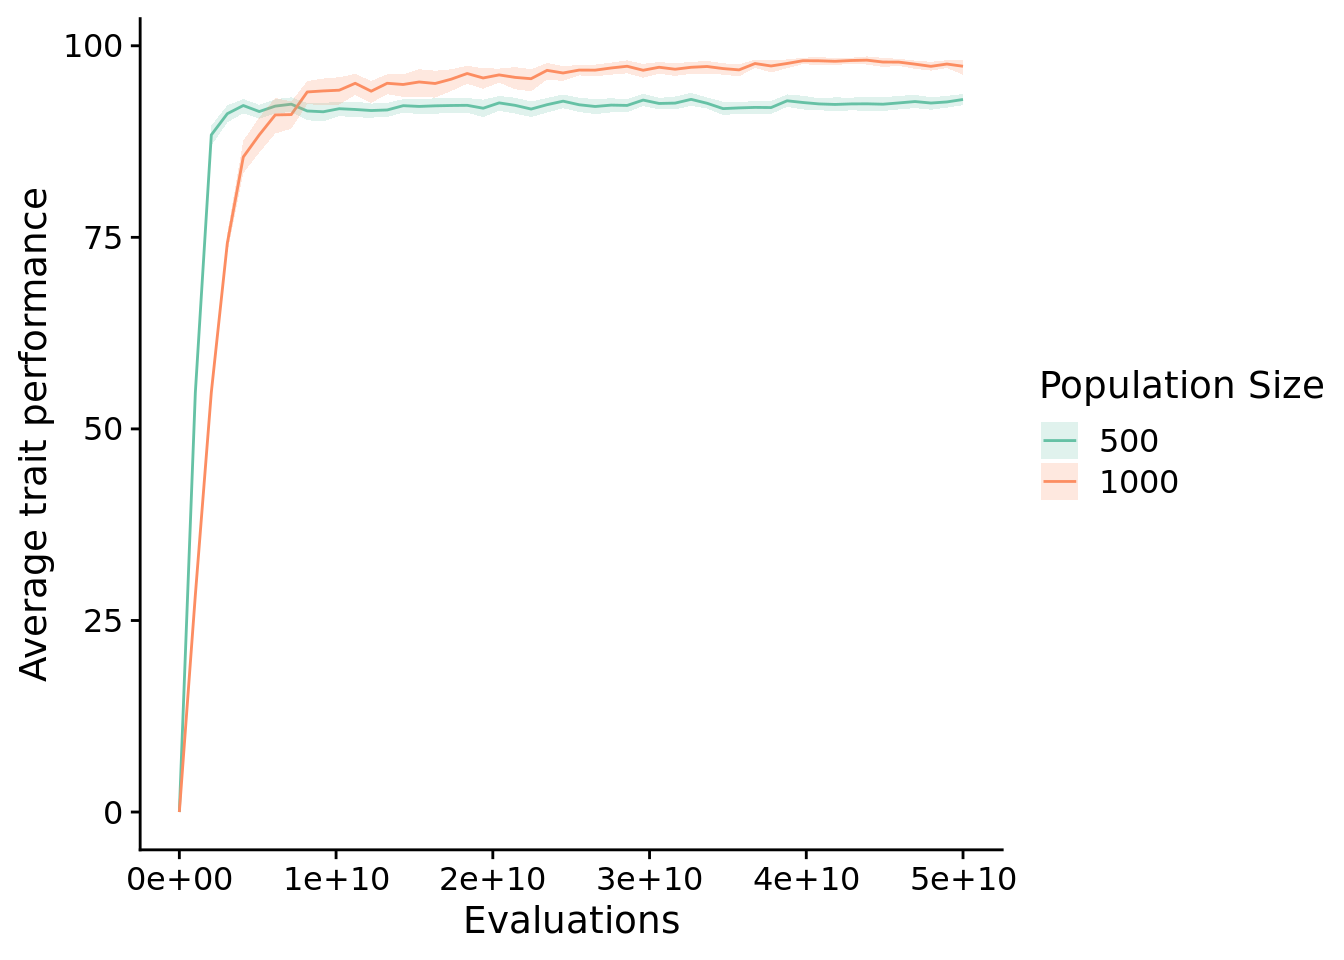
\includegraphics{supplemental-material_files/figure-latex/unnamed-chunk-35-1.pdf}

Same as above, but by generations instead of evaluations.

\begin{Shaded}
\begin{Highlighting}[]
\KeywordTok{ggplot}\NormalTok{(data, }\KeywordTok{aes}\NormalTok{(}\DataTypeTok{x=}\NormalTok{gen, }\DataTypeTok{y=}\NormalTok{elite_trait_avg, }\DataTypeTok{color=}\NormalTok{POP_SIZE)) }\OperatorTok{+}
\StringTok{  }\KeywordTok{stat_summary}\NormalTok{(}\DataTypeTok{geom=}\StringTok{"line"}\NormalTok{, }\DataTypeTok{fun=}\NormalTok{mean) }\OperatorTok{+}
\StringTok{  }\KeywordTok{stat_summary}\NormalTok{(}
    \DataTypeTok{geom=}\StringTok{"ribbon"}\NormalTok{,}
    \DataTypeTok{fun.data=}\StringTok{"mean_cl_boot"}\NormalTok{,}
    \DataTypeTok{fun.args=}\KeywordTok{list}\NormalTok{(}\DataTypeTok{conf.int=}\FloatTok{0.95}\NormalTok{),}
    \DataTypeTok{alpha=}\FloatTok{0.2}\NormalTok{,}
    \DataTypeTok{linetype=}\DecValTok{0}
\NormalTok{  ) }\OperatorTok{+}
\StringTok{  }\KeywordTok{scale_y_continuous}\NormalTok{(}
    \DataTypeTok{name=}\StringTok{"Elite trait average"}
\NormalTok{  ) }\OperatorTok{+}
\StringTok{  }\KeywordTok{scale_x_continuous}\NormalTok{(}
    \DataTypeTok{name=}\StringTok{"Generations"}
\NormalTok{  )}
\end{Highlighting}
\end{Shaded}

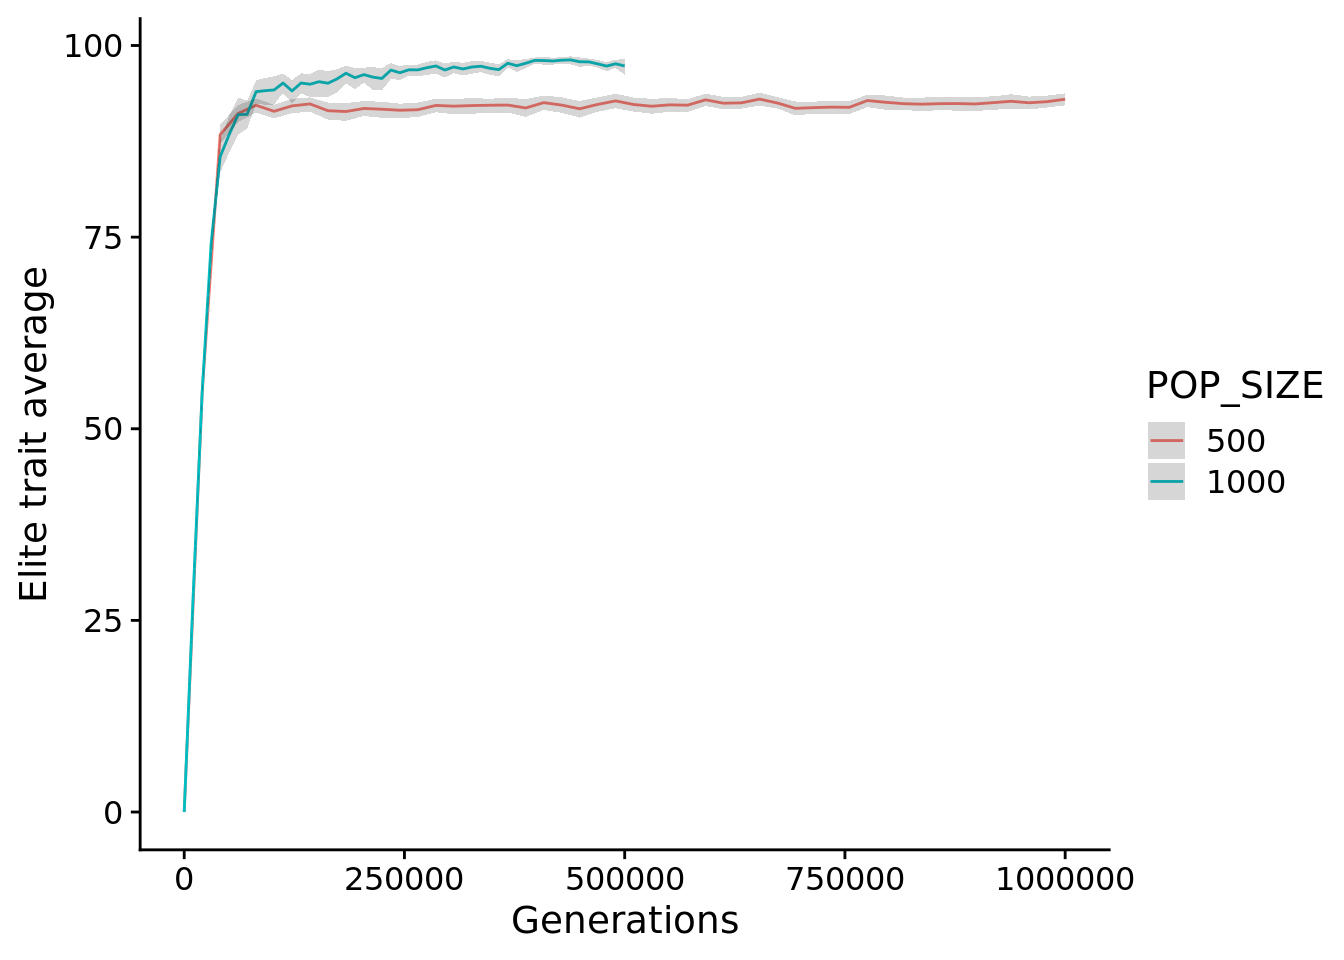
\includegraphics{supplemental-material_files/figure-latex/unnamed-chunk-36-1.pdf}

\hypertarget{final-performance-2}{%
\subsection{Final performance}\label{final-performance-2}}

\begin{Shaded}
\begin{Highlighting}[]
\NormalTok{elite_final_performance_fig <-}\StringTok{ }\KeywordTok{ggplot}\NormalTok{(}
\NormalTok{    final_data,}
    \KeywordTok{aes}\NormalTok{(}\DataTypeTok{x=}\NormalTok{POP_SIZE, }\DataTypeTok{y=}\NormalTok{elite_trait_avg, }\DataTypeTok{fill=}\NormalTok{POP_SIZE)}
\NormalTok{  ) }\OperatorTok{+}
\StringTok{  }\KeywordTok{geom_flat_violin}\NormalTok{(}
    \DataTypeTok{position =} \KeywordTok{position_nudge}\NormalTok{(}\DataTypeTok{x =} \FloatTok{.2}\NormalTok{, }\DataTypeTok{y =} \DecValTok{0}\NormalTok{),}
    \DataTypeTok{alpha =} \FloatTok{.8}\NormalTok{,}
    \DataTypeTok{scale=}\StringTok{"width"}
\NormalTok{  ) }\OperatorTok{+}
\StringTok{  }\KeywordTok{geom_point}\NormalTok{(}
    \DataTypeTok{mapping=}\KeywordTok{aes}\NormalTok{(}\DataTypeTok{color=}\NormalTok{POP_SIZE),}
    \DataTypeTok{position =} \KeywordTok{position_jitter}\NormalTok{(}\DataTypeTok{width =} \FloatTok{.15}\NormalTok{),}
    \DataTypeTok{size =} \FloatTok{.5}\NormalTok{,}
    \DataTypeTok{alpha =} \FloatTok{0.8}
\NormalTok{  ) }\OperatorTok{+}
\StringTok{  }\KeywordTok{geom_boxplot}\NormalTok{(}
    \DataTypeTok{width =} \FloatTok{.1}\NormalTok{,}
    \DataTypeTok{outlier.shape =} \OtherTok{NA}\NormalTok{,}
    \DataTypeTok{alpha =} \FloatTok{0.5}
\NormalTok{  ) }\OperatorTok{+}
\StringTok{  }\KeywordTok{scale_y_continuous}\NormalTok{(}
    \DataTypeTok{name=}\StringTok{"Average trait performance"}\NormalTok{,}
    \DataTypeTok{limits=}\KeywordTok{c}\NormalTok{(}\DecValTok{0}\NormalTok{, }\DecValTok{100}\NormalTok{)}
\NormalTok{  ) }\OperatorTok{+}
\StringTok{  }\KeywordTok{scale_x_discrete}\NormalTok{(}
    \DataTypeTok{name=}\StringTok{"Population Size"}
\NormalTok{  ) }\OperatorTok{+}
\StringTok{  }\KeywordTok{scale_fill_brewer}\NormalTok{(}
    \DataTypeTok{name=}\StringTok{"Population Size"}\NormalTok{,}
    \DataTypeTok{palette=}\NormalTok{cb_palette}
\NormalTok{  ) }\OperatorTok{+}
\StringTok{  }\KeywordTok{scale_color_brewer}\NormalTok{(}
    \DataTypeTok{name=}\StringTok{"Population Size"}\NormalTok{,}
    \DataTypeTok{palette=}\NormalTok{cb_palette}
\NormalTok{  ) }\OperatorTok{+}
\StringTok{  }\KeywordTok{theme}\NormalTok{(}
    \DataTypeTok{legend.position=}\StringTok{"none"}
\NormalTok{  )}
\NormalTok{elite_final_performance_fig}
\end{Highlighting}
\end{Shaded}

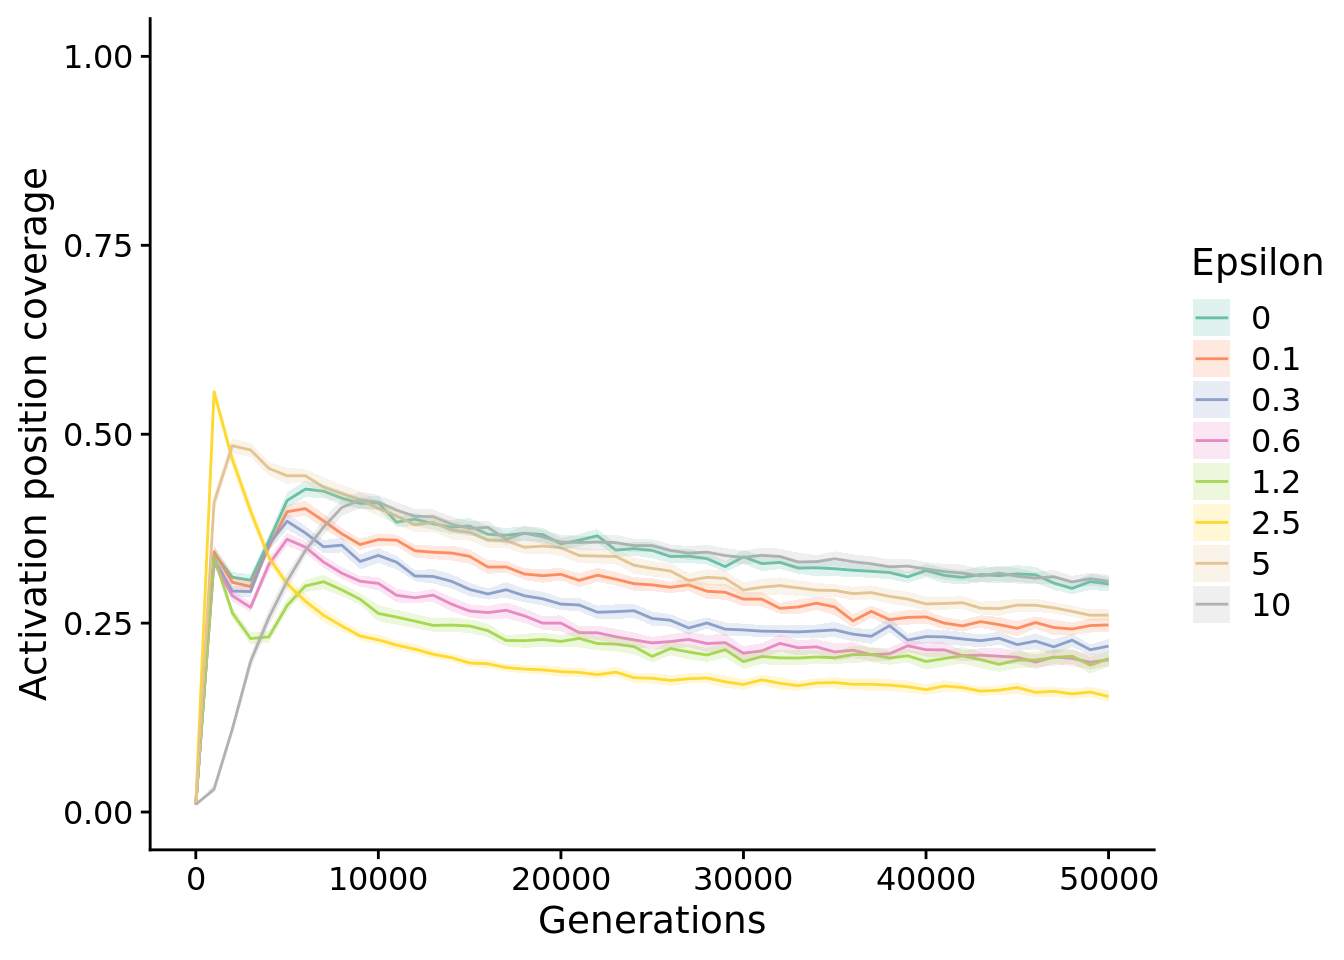
\includegraphics{supplemental-material_files/figure-latex/unnamed-chunk-37-1.pdf}

\hypertarget{unique-starting-positions-2}{%
\section{Unique starting positions}\label{unique-starting-positions-2}}

\begin{Shaded}
\begin{Highlighting}[]
\NormalTok{unique_start_position_coverage_fig <-}\StringTok{ }\KeywordTok{ggplot}\NormalTok{(}
\NormalTok{    data,}
    \KeywordTok{aes}\NormalTok{(}
      \DataTypeTok{x=}\NormalTok{evaluations,}
      \DataTypeTok{y=}\NormalTok{unique_start_positions_coverage,}
      \DataTypeTok{color=}\NormalTok{POP_SIZE,}
      \DataTypeTok{fill=}\NormalTok{POP_SIZE}
\NormalTok{    )}
\NormalTok{  ) }\OperatorTok{+}
\StringTok{  }\KeywordTok{stat_summary}\NormalTok{(}\DataTypeTok{geom=}\StringTok{"line"}\NormalTok{, }\DataTypeTok{fun=}\NormalTok{mean) }\OperatorTok{+}
\StringTok{  }\KeywordTok{stat_summary}\NormalTok{(}
    \DataTypeTok{geom=}\StringTok{"ribbon"}\NormalTok{,}
    \DataTypeTok{fun.data=}\StringTok{"mean_cl_boot"}\NormalTok{,}
    \DataTypeTok{fun.args=}\KeywordTok{list}\NormalTok{(}\DataTypeTok{conf.int=}\FloatTok{0.95}\NormalTok{),}
    \DataTypeTok{alpha=}\FloatTok{0.2}\NormalTok{,}
    \DataTypeTok{linetype=}\DecValTok{0}
\NormalTok{  ) }\OperatorTok{+}
\StringTok{  }\KeywordTok{scale_y_continuous}\NormalTok{(}
    \DataTypeTok{name=}\StringTok{"Activation position coverage"}\NormalTok{,}
    \DataTypeTok{limits=}\KeywordTok{c}\NormalTok{(}\FloatTok{0.0}\NormalTok{, }\FloatTok{1.0}\NormalTok{)}
\NormalTok{  ) }\OperatorTok{+}
\StringTok{  }\KeywordTok{scale_x_continuous}\NormalTok{(}
    \DataTypeTok{name=}\StringTok{"Evaluations"}
\NormalTok{  ) }\OperatorTok{+}
\StringTok{  }\KeywordTok{scale_fill_brewer}\NormalTok{(}
    \DataTypeTok{name=}\StringTok{"Population Size"}\NormalTok{,}
    \DataTypeTok{palette=}\NormalTok{cb_palette}
\NormalTok{  ) }\OperatorTok{+}
\StringTok{  }\KeywordTok{scale_color_brewer}\NormalTok{(}
    \DataTypeTok{name=}\StringTok{"Population Size"}\NormalTok{,}
    \DataTypeTok{palette=}\NormalTok{cb_palette}
\NormalTok{  )}
\NormalTok{unique_start_position_coverage_fig}
\end{Highlighting}
\end{Shaded}

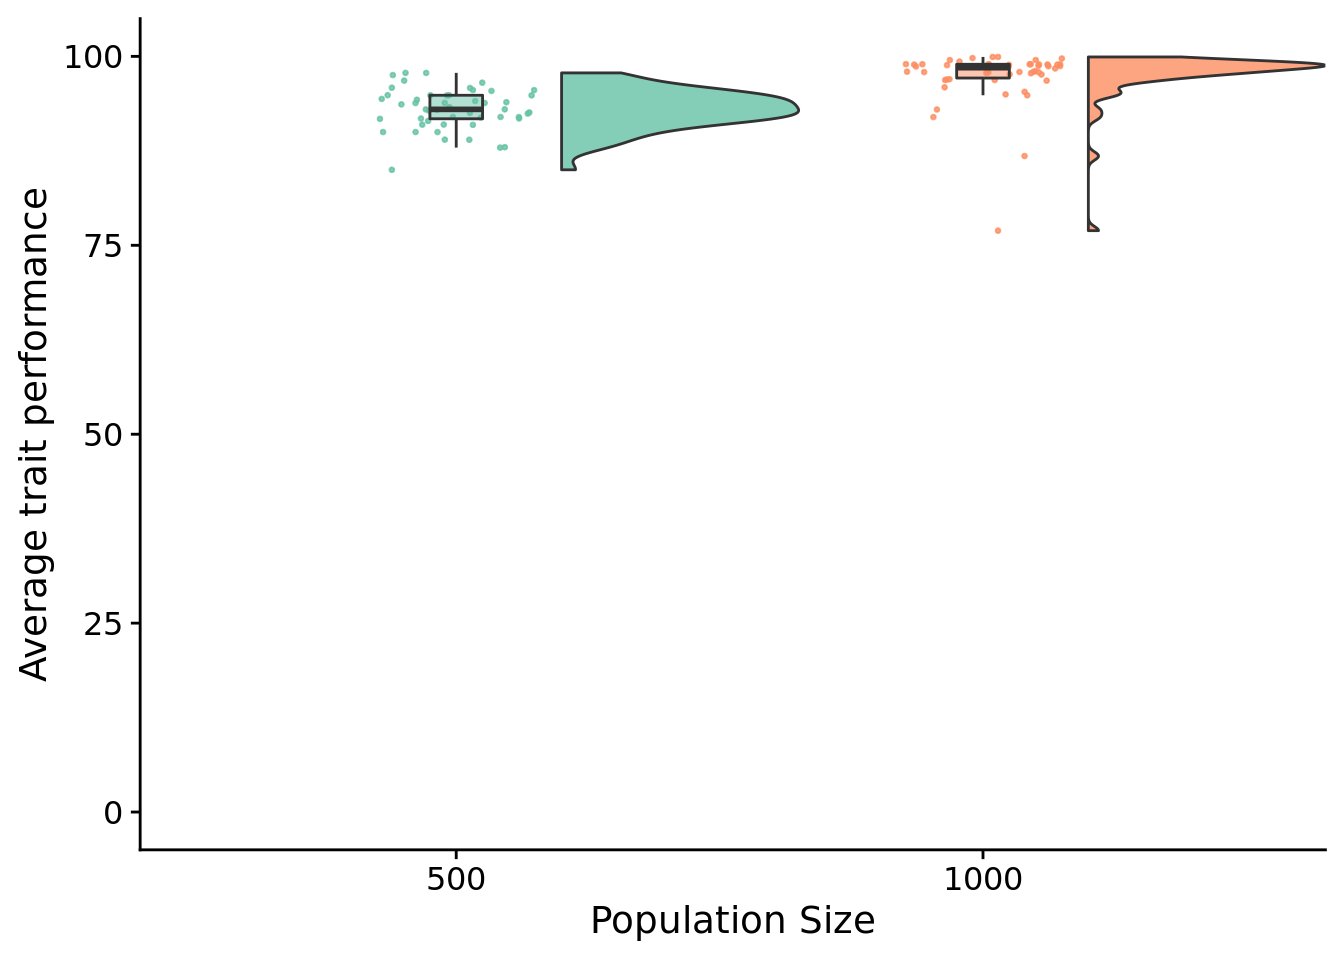
\includegraphics{supplemental-material_files/figure-latex/unnamed-chunk-38-1.pdf}

\hypertarget{final-starting-position-coverage-2}{%
\subsection{Final starting position coverage}\label{final-starting-position-coverage-2}}

\begin{Shaded}
\begin{Highlighting}[]
\NormalTok{unique_start_positions_coverage_final_fig <-}\StringTok{ }\KeywordTok{ggplot}\NormalTok{(}
\NormalTok{    final_data,}
    \KeywordTok{aes}\NormalTok{(}
      \DataTypeTok{x=}\NormalTok{POP_SIZE,}
      \DataTypeTok{y=}\NormalTok{unique_start_positions_coverage,}
      \DataTypeTok{fill=}\NormalTok{POP_SIZE}
\NormalTok{    )}
\NormalTok{  ) }\OperatorTok{+}
\StringTok{  }\KeywordTok{geom_flat_violin}\NormalTok{(}
    \DataTypeTok{position =} \KeywordTok{position_nudge}\NormalTok{(}\DataTypeTok{x =} \FloatTok{.2}\NormalTok{, }\DataTypeTok{y =} \DecValTok{0}\NormalTok{),}
    \DataTypeTok{alpha =} \FloatTok{.8}\NormalTok{,}
    \DataTypeTok{scale=}\StringTok{"width"}
\NormalTok{  ) }\OperatorTok{+}
\StringTok{  }\KeywordTok{geom_point}\NormalTok{(}
    \DataTypeTok{mapping=}\KeywordTok{aes}\NormalTok{(}\DataTypeTok{color=}\NormalTok{POP_SIZE),}
    \DataTypeTok{position =} \KeywordTok{position_jitter}\NormalTok{(}\DataTypeTok{width =} \FloatTok{.15}\NormalTok{),}
    \DataTypeTok{size =} \FloatTok{.5}\NormalTok{,}
    \DataTypeTok{alpha =} \FloatTok{0.8}
\NormalTok{  ) }\OperatorTok{+}
\StringTok{  }\KeywordTok{geom_boxplot}\NormalTok{(}
    \DataTypeTok{width =} \FloatTok{.1}\NormalTok{,}
    \DataTypeTok{outlier.shape =} \OtherTok{NA}\NormalTok{,}
    \DataTypeTok{alpha =} \FloatTok{0.5}
\NormalTok{  ) }\OperatorTok{+}
\StringTok{  }\KeywordTok{scale_y_continuous}\NormalTok{(}
    \DataTypeTok{name=}\StringTok{"Activation position coverage"}\NormalTok{,}
    \DataTypeTok{limits=}\KeywordTok{c}\NormalTok{(}\DecValTok{0}\NormalTok{, }\FloatTok{1.0}\NormalTok{)}
\NormalTok{  ) }\OperatorTok{+}
\StringTok{  }\KeywordTok{scale_x_discrete}\NormalTok{(}
    \DataTypeTok{name=}\StringTok{"Population size"}
\NormalTok{  ) }\OperatorTok{+}
\StringTok{  }\KeywordTok{scale_fill_brewer}\NormalTok{(}
    \DataTypeTok{name=}\StringTok{"Population size"}\NormalTok{,}
    \DataTypeTok{palette=}\NormalTok{cb_palette}
\NormalTok{  ) }\OperatorTok{+}
\StringTok{  }\KeywordTok{scale_color_brewer}\NormalTok{(}
    \DataTypeTok{name=}\StringTok{"Population size"}\NormalTok{,}
    \DataTypeTok{palette=}\NormalTok{cb_palette}
\NormalTok{  ) }\OperatorTok{+}
\StringTok{  }\KeywordTok{theme}\NormalTok{(}
    \DataTypeTok{legend.position=}\StringTok{"none"}
\NormalTok{  )}
\NormalTok{unique_start_positions_coverage_final_fig}
\end{Highlighting}
\end{Shaded}

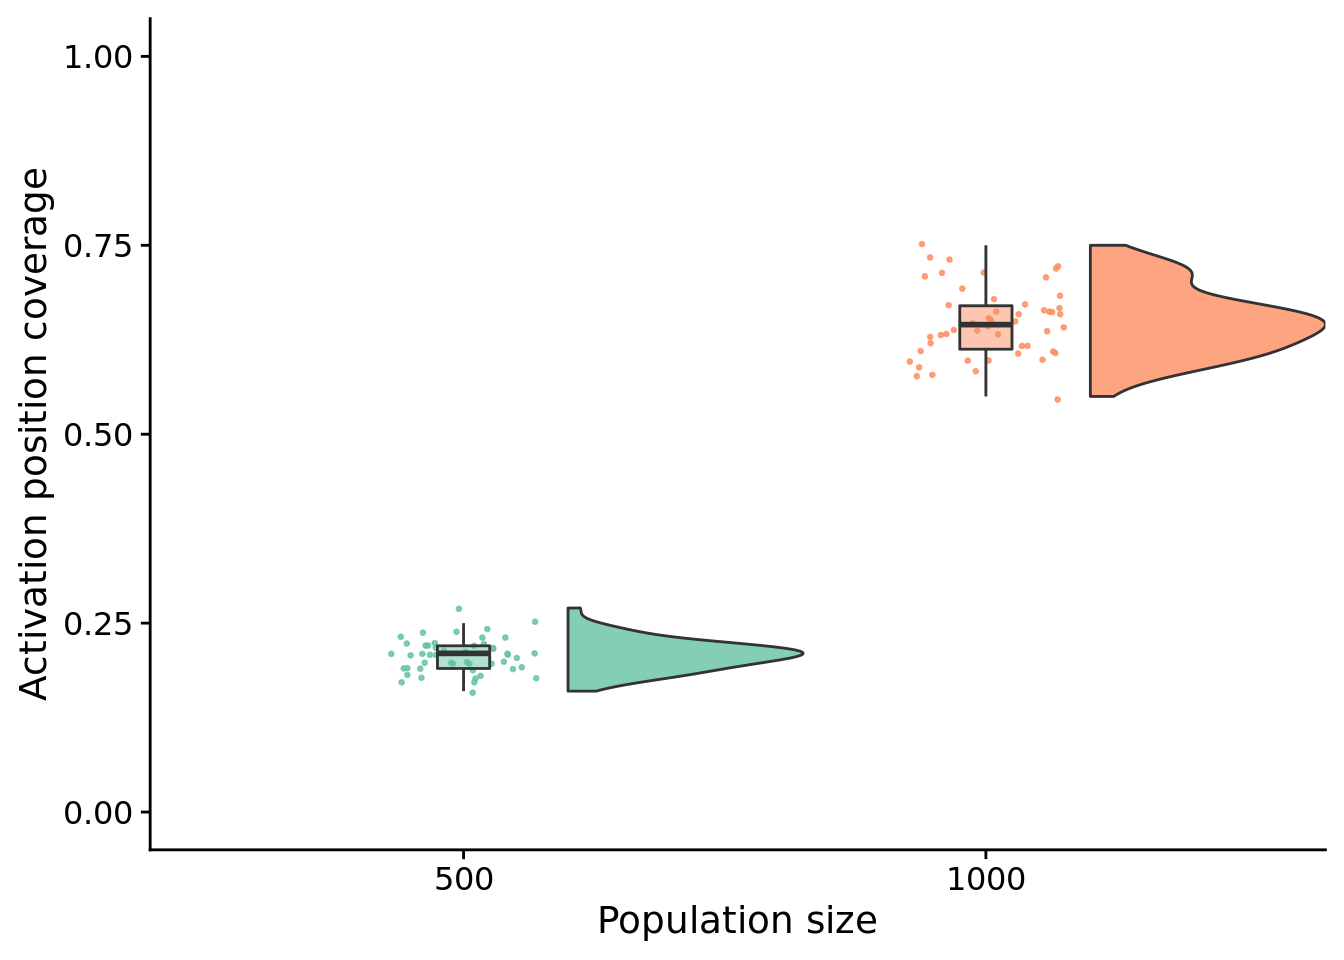
\includegraphics{supplemental-material_files/figure-latex/unnamed-chunk-39-1.pdf}

\hypertarget{manuscript-figures-2}{%
\section{Manuscript figures}\label{manuscript-figures-2}}

\begin{Shaded}
\begin{Highlighting}[]
\NormalTok{legend <-}\StringTok{ }\NormalTok{cowplot}\OperatorTok{::}\KeywordTok{get_legend}\NormalTok{(}
\NormalTok{    elite_ave_performance_fig }\OperatorTok{+}
\StringTok{      }\KeywordTok{guides}\NormalTok{(}
        \DataTypeTok{color=}\KeywordTok{guide_legend}\NormalTok{(}\DataTypeTok{nrow=}\DecValTok{1}\NormalTok{),}
        \DataTypeTok{fill=}\KeywordTok{guide_legend}\NormalTok{(}\DataTypeTok{nrow=}\DecValTok{1}\NormalTok{)}
\NormalTok{      ) }\OperatorTok{+}
\StringTok{      }\KeywordTok{theme}\NormalTok{(}
        \DataTypeTok{legend.position =} \StringTok{"bottom"}\NormalTok{,}
        \DataTypeTok{legend.box=}\StringTok{"horizontal"}\NormalTok{,}
        \DataTypeTok{legend.justification=}\StringTok{"center"}
\NormalTok{      )}
\NormalTok{  )}

\NormalTok{grid <-}\StringTok{ }\KeywordTok{plot_grid}\NormalTok{(}
\NormalTok{  elite_ave_performance_fig }\OperatorTok{+}
\StringTok{    }\KeywordTok{ggtitle}\NormalTok{(}\StringTok{"Performance over time"}\NormalTok{) }\OperatorTok{+}
\StringTok{    }\KeywordTok{theme}\NormalTok{(}\DataTypeTok{legend.position=}\StringTok{"none"}\NormalTok{),}
\NormalTok{  elite_final_performance_fig }\OperatorTok{+}
\StringTok{    }\KeywordTok{ggtitle}\NormalTok{(}\StringTok{"Final performance"}\NormalTok{) }\OperatorTok{+}
\StringTok{    }\KeywordTok{theme}\NormalTok{(),}
\NormalTok{  unique_start_position_coverage_fig }\OperatorTok{+}
\StringTok{    }\KeywordTok{ggtitle}\NormalTok{(}\StringTok{"Activation position coverage over time"}\NormalTok{) }\OperatorTok{+}
\StringTok{    }\KeywordTok{theme}\NormalTok{(}\DataTypeTok{legend.position=}\StringTok{"none"}\NormalTok{),}
\NormalTok{  unique_start_positions_coverage_final_fig }\OperatorTok{+}
\StringTok{    }\KeywordTok{ggtitle}\NormalTok{(}\StringTok{"Final activation position coverage"}\NormalTok{) }\OperatorTok{+}
\StringTok{    }\KeywordTok{theme}\NormalTok{(),}
  \DataTypeTok{nrow=}\DecValTok{2}\NormalTok{,}
  \DataTypeTok{ncol=}\DecValTok{2}\NormalTok{,}
  \DataTypeTok{rel_widths=}\KeywordTok{c}\NormalTok{(}\DecValTok{3}\NormalTok{,}\DecValTok{2}\NormalTok{),}
  \DataTypeTok{labels=}\StringTok{"auto"}
\NormalTok{)}

\NormalTok{grid <-}\StringTok{ }\KeywordTok{plot_grid}\NormalTok{(}
\NormalTok{  grid,}
\NormalTok{  legend,}
  \DataTypeTok{nrow=}\DecValTok{2}\NormalTok{,}
  \DataTypeTok{ncol=}\DecValTok{1}\NormalTok{,}
  \DataTypeTok{rel_heights=}\KeywordTok{c}\NormalTok{(}\DecValTok{1}\NormalTok{, }\FloatTok{0.1}\NormalTok{)}
\NormalTok{)}


\KeywordTok{save_plot}\NormalTok{(}
  \KeywordTok{paste}\NormalTok{(working_directory, }\StringTok{"imgs/pop-size-panel.pdf"}\NormalTok{, }\DataTypeTok{sep=}\StringTok{""}\NormalTok{),}
\NormalTok{  grid,}
  \DataTypeTok{base_width=}\DecValTok{12}\NormalTok{,}
  \DataTypeTok{base_height=}\DecValTok{8}
\NormalTok{)}

\NormalTok{grid}
\end{Highlighting}
\end{Shaded}

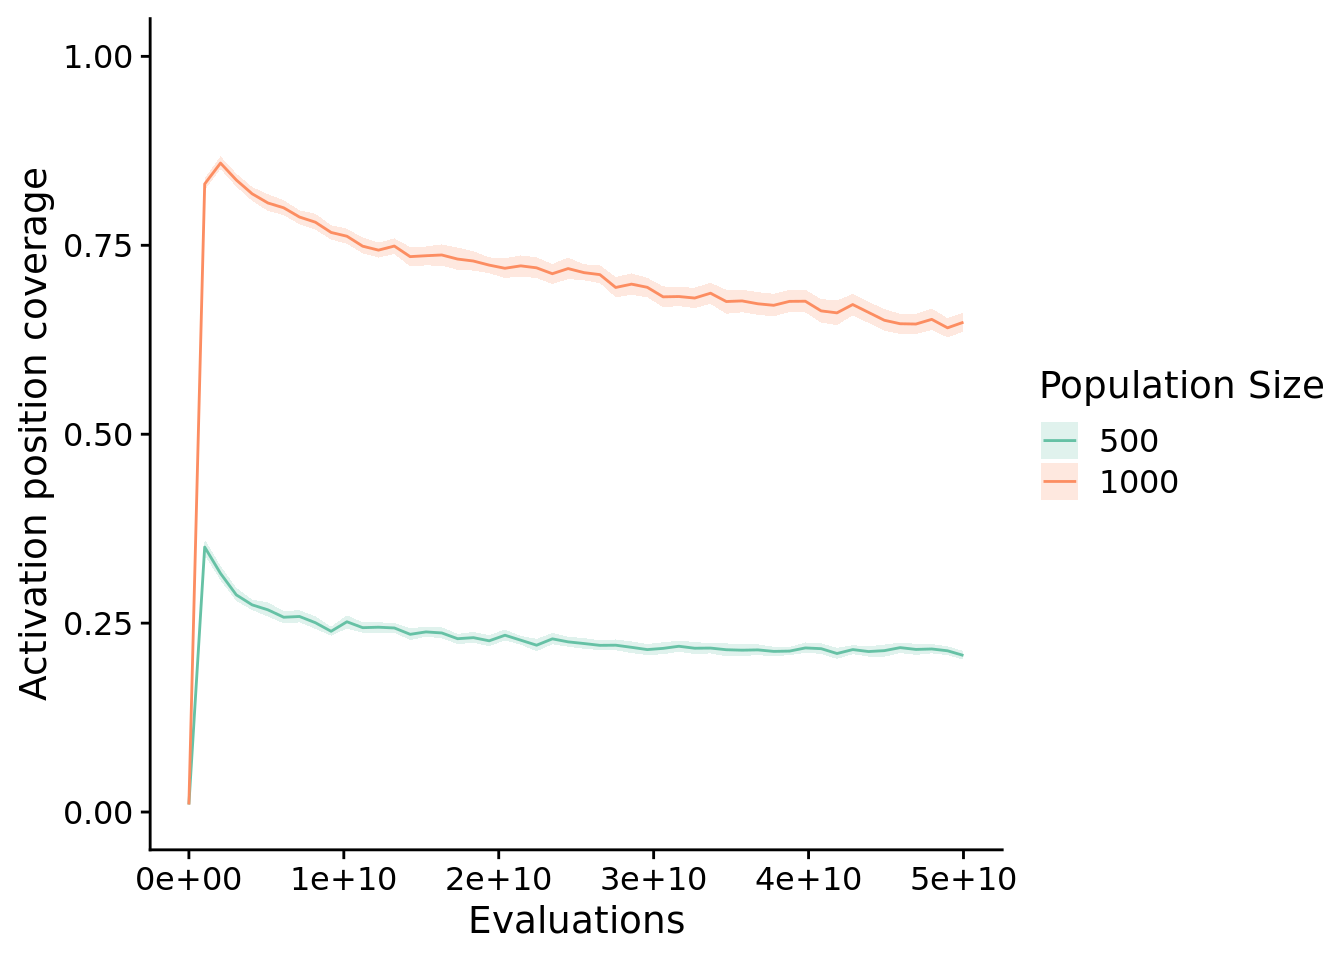
\includegraphics{supplemental-material_files/figure-latex/unnamed-chunk-40-1.pdf}

\hypertarget{epsilon-lexicase}{%
\chapter{Epsilon lexicase}\label{epsilon-lexicase}}

\hypertarget{overview-3}{%
\section{Overview}\label{overview-3}}

\begin{Shaded}
\begin{Highlighting}[]
\CommentTok{# Relative location of data.}
\NormalTok{working_directory <-}\StringTok{ "experiments/2021-05-28-epsilon/analysis/"}
\CommentTok{# working_directory <- "./"}

\CommentTok{# Settings for visualization}
\NormalTok{cb_palette <-}\StringTok{ "Set2"}
\CommentTok{# Create directory to dump plots}
\KeywordTok{dir.create}\NormalTok{(}\KeywordTok{paste0}\NormalTok{(working_directory, }\StringTok{"imgs"}\NormalTok{), }\DataTypeTok{showWarnings=}\OtherTok{FALSE}\NormalTok{)}
\end{Highlighting}
\end{Shaded}

\hypertarget{analysis-dependencies-3}{%
\section{Analysis dependencies}\label{analysis-dependencies-3}}

\begin{Shaded}
\begin{Highlighting}[]
\KeywordTok{library}\NormalTok{(ggplot2)}
\KeywordTok{library}\NormalTok{(tidyverse)}
\KeywordTok{library}\NormalTok{(cowplot)}
\KeywordTok{library}\NormalTok{(viridis)}
\KeywordTok{library}\NormalTok{(RColorBrewer)}
\KeywordTok{source}\NormalTok{(}\StringTok{"https://gist.githubusercontent.com/benmarwick/2a1bb0133ff568cbe28d/raw/fb53bd97121f7f9ce947837ef1a4c65a73bffb3f/geom_flat_violin.R"}\NormalTok{)}
\end{Highlighting}
\end{Shaded}

These analyses were conducted in the following computing environment:

\begin{Shaded}
\begin{Highlighting}[]
\KeywordTok{print}\NormalTok{(version)}
\end{Highlighting}
\end{Shaded}

\begin{verbatim}
##                _                           
## platform       x86_64-pc-linux-gnu         
## arch           x86_64                      
## os             linux-gnu                   
## system         x86_64, linux-gnu           
## status                                     
## major          4                           
## minor          1.0                         
## year           2021                        
## month          05                          
## day            18                          
## svn rev        80317                       
## language       R                           
## version.string R version 4.1.0 (2021-05-18)
## nickname       Camp Pontanezen
\end{verbatim}

\hypertarget{setup-3}{%
\section{Setup}\label{setup-3}}

\begin{Shaded}
\begin{Highlighting}[]
\NormalTok{data_loc <-}\StringTok{ }\KeywordTok{paste0}\NormalTok{(}
\NormalTok{  working_directory,}
  \StringTok{"data/timeseries-res-1000g.csv"}
\NormalTok{)}
\NormalTok{data <-}\StringTok{ }\KeywordTok{read.csv}\NormalTok{(data_loc, }\DataTypeTok{na.strings=}\StringTok{"NONE"}\NormalTok{)}

\NormalTok{data}\OperatorTok{$}\NormalTok{cardinality <-}\StringTok{ }\KeywordTok{as.factor}\NormalTok{(}
\NormalTok{  data}\OperatorTok{$}\NormalTok{OBJECTIVE_CNT}
\NormalTok{)}
\NormalTok{data}\OperatorTok{$}\NormalTok{selection_name <-}\StringTok{ }\KeywordTok{as.factor}\NormalTok{(}
\NormalTok{  data}\OperatorTok{$}\NormalTok{selection_name}
\NormalTok{)}

\NormalTok{data}\OperatorTok{$}\NormalTok{epsilon <-}\StringTok{ }\KeywordTok{as.factor}\NormalTok{(}
\NormalTok{  data}\OperatorTok{$}\NormalTok{LEX_EPS}
\NormalTok{)}

\NormalTok{data}\OperatorTok{$}\NormalTok{elite_trait_avg <-}
\StringTok{  }\NormalTok{data}\OperatorTok{$}\NormalTok{ele_agg_per }\OperatorTok{/}\StringTok{ }\NormalTok{data}\OperatorTok{$}\NormalTok{OBJECTIVE_CNT}
\NormalTok{data}\OperatorTok{$}\NormalTok{unique_start_positions_coverage <-}
\StringTok{  }\NormalTok{data}\OperatorTok{$}\NormalTok{uni_str_pos }\OperatorTok{/}\StringTok{ }\NormalTok{data}\OperatorTok{$}\NormalTok{OBJECTIVE_CNT}

\NormalTok{final_data <-}\StringTok{ }\KeywordTok{filter}\NormalTok{(data, evaluations}\OperatorTok{==}\KeywordTok{max}\NormalTok{(data}\OperatorTok{$}\NormalTok{evaluations))}

\CommentTok{####### misc #######}
\CommentTok{# Configure our default graphing theme}
\KeywordTok{theme_set}\NormalTok{(}\KeywordTok{theme_cowplot}\NormalTok{())}
\end{Highlighting}
\end{Shaded}

\hypertarget{exploration-diagnostic-performance-3}{%
\section{Exploration diagnostic performance}\label{exploration-diagnostic-performance-3}}

\begin{Shaded}
\begin{Highlighting}[]
\NormalTok{elite_ave_performance_fig <-}
\StringTok{  }\KeywordTok{ggplot}\NormalTok{(}
\NormalTok{    data,}
    \KeywordTok{aes}\NormalTok{(}\DataTypeTok{x=}\NormalTok{gen, }\DataTypeTok{y=}\NormalTok{elite_trait_avg, }\DataTypeTok{color=}\NormalTok{epsilon, }\DataTypeTok{fill=}\NormalTok{epsilon)}
\NormalTok{  ) }\OperatorTok{+}
\StringTok{  }\KeywordTok{stat_summary}\NormalTok{(}\DataTypeTok{geom=}\StringTok{"line"}\NormalTok{, }\DataTypeTok{fun=}\NormalTok{mean) }\OperatorTok{+}
\StringTok{  }\KeywordTok{stat_summary}\NormalTok{(}
    \DataTypeTok{geom=}\StringTok{"ribbon"}\NormalTok{,}
    \DataTypeTok{fun.data=}\StringTok{"mean_cl_boot"}\NormalTok{,}
    \DataTypeTok{fun.args=}\KeywordTok{list}\NormalTok{(}\DataTypeTok{conf.int=}\FloatTok{0.95}\NormalTok{),}
    \DataTypeTok{alpha=}\FloatTok{0.2}\NormalTok{,}
    \DataTypeTok{linetype=}\DecValTok{0}
\NormalTok{  ) }\OperatorTok{+}
\StringTok{  }\KeywordTok{scale_y_continuous}\NormalTok{(}
    \DataTypeTok{name=}\StringTok{"Average trait performance"}
\NormalTok{  ) }\OperatorTok{+}
\StringTok{  }\KeywordTok{scale_x_continuous}\NormalTok{(}
    \DataTypeTok{name=}\StringTok{"Generations"}
\NormalTok{  ) }\OperatorTok{+}
\StringTok{  }\KeywordTok{scale_fill_brewer}\NormalTok{(}
    \DataTypeTok{name=}\StringTok{"Epsilon"}\NormalTok{,}
    \DataTypeTok{palette=}\NormalTok{cb_palette}
\NormalTok{  ) }\OperatorTok{+}
\StringTok{  }\KeywordTok{scale_color_brewer}\NormalTok{(}
    \DataTypeTok{name=}\StringTok{"Epsilon"}\NormalTok{,}
    \DataTypeTok{palette=}\NormalTok{cb_palette}
\NormalTok{  )}
\NormalTok{elite_ave_performance_fig}
\end{Highlighting}
\end{Shaded}

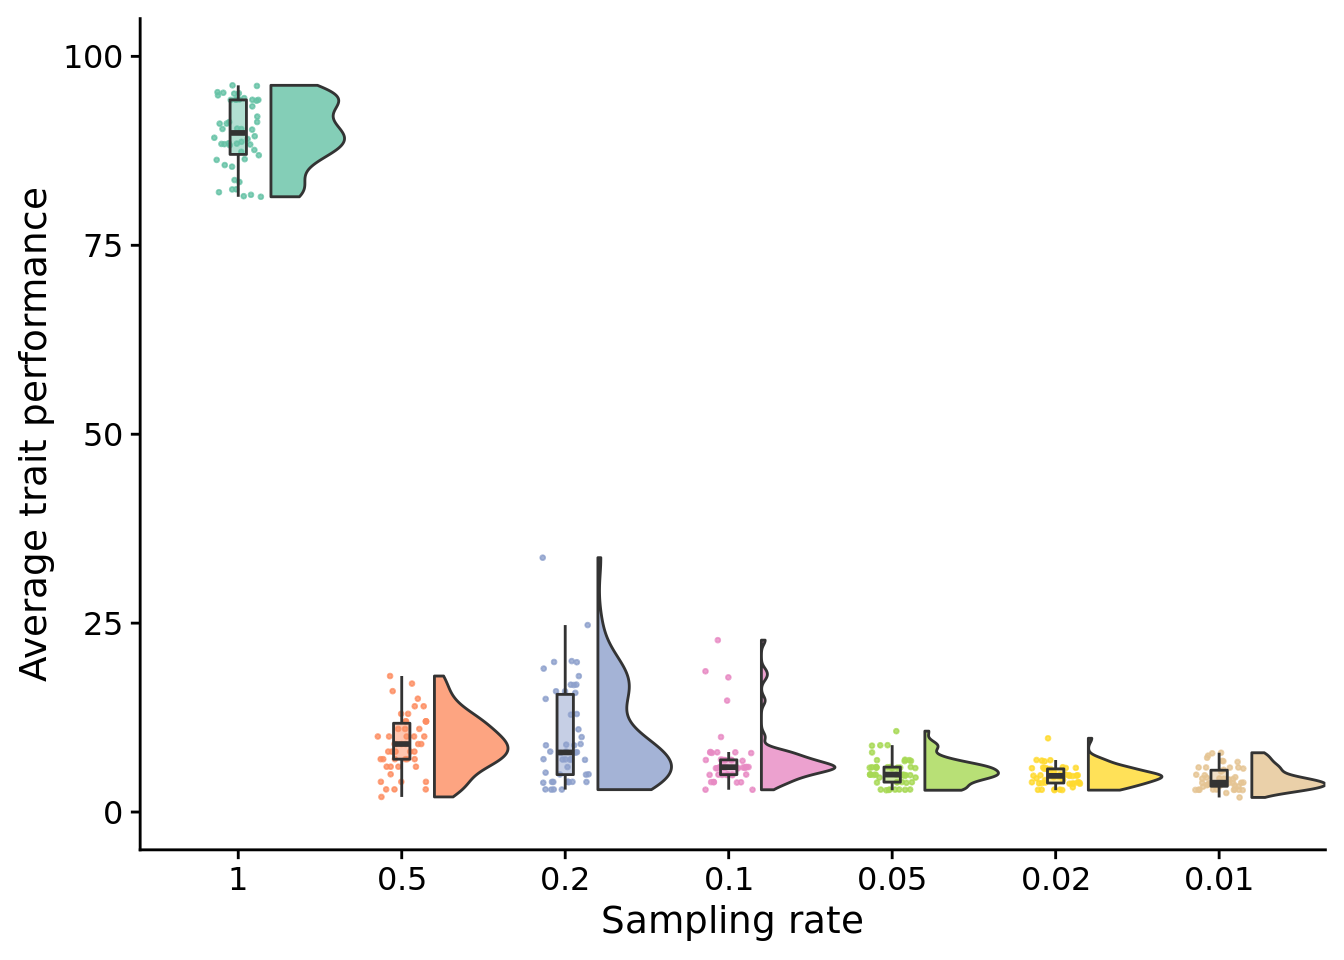
\includegraphics{supplemental-material_files/figure-latex/unnamed-chunk-45-1.pdf}

\hypertarget{final-performance-3}{%
\subsection{Final performance}\label{final-performance-3}}

\begin{Shaded}
\begin{Highlighting}[]
\NormalTok{elite_final_performance_fig <-}\StringTok{ }\KeywordTok{ggplot}\NormalTok{(}
\NormalTok{    final_data,}
    \KeywordTok{aes}\NormalTok{(}\DataTypeTok{x=}\NormalTok{epsilon, }\DataTypeTok{y=}\NormalTok{elite_trait_avg, }\DataTypeTok{fill=}\NormalTok{epsilon)}
\NormalTok{  ) }\OperatorTok{+}
\StringTok{  }\KeywordTok{geom_flat_violin}\NormalTok{(}
    \DataTypeTok{position =} \KeywordTok{position_nudge}\NormalTok{(}\DataTypeTok{x =} \FloatTok{.2}\NormalTok{, }\DataTypeTok{y =} \DecValTok{0}\NormalTok{),}
    \DataTypeTok{alpha =} \FloatTok{.8}\NormalTok{,}
    \DataTypeTok{scale=}\StringTok{"width"}
\NormalTok{  ) }\OperatorTok{+}
\StringTok{  }\KeywordTok{geom_point}\NormalTok{(}
    \DataTypeTok{mapping=}\KeywordTok{aes}\NormalTok{(}\DataTypeTok{color=}\NormalTok{epsilon),}
    \DataTypeTok{position =} \KeywordTok{position_jitter}\NormalTok{(}\DataTypeTok{width =} \FloatTok{.15}\NormalTok{),}
    \DataTypeTok{size =} \FloatTok{.5}\NormalTok{,}
    \DataTypeTok{alpha =} \FloatTok{0.8}
\NormalTok{  ) }\OperatorTok{+}
\StringTok{  }\KeywordTok{geom_boxplot}\NormalTok{(}
    \DataTypeTok{width =} \FloatTok{.1}\NormalTok{,}
    \DataTypeTok{outlier.shape =} \OtherTok{NA}\NormalTok{,}
    \DataTypeTok{alpha =} \FloatTok{0.5}
\NormalTok{  ) }\OperatorTok{+}
\StringTok{  }\KeywordTok{scale_y_continuous}\NormalTok{(}
    \DataTypeTok{name=}\StringTok{"Average trait performance"}\NormalTok{,}
    \DataTypeTok{limits=}\KeywordTok{c}\NormalTok{(}\DecValTok{0}\NormalTok{, }\DecValTok{100}\NormalTok{)}
\NormalTok{  ) }\OperatorTok{+}
\StringTok{  }\KeywordTok{scale_x_discrete}\NormalTok{(}
    \DataTypeTok{name=}\StringTok{"Epsilon"}
\NormalTok{  ) }\OperatorTok{+}
\StringTok{  }\KeywordTok{scale_fill_brewer}\NormalTok{(}
    \DataTypeTok{name=}\StringTok{"Epsilon"}\NormalTok{,}
    \DataTypeTok{palette=}\NormalTok{cb_palette}
\NormalTok{  ) }\OperatorTok{+}
\StringTok{  }\KeywordTok{scale_color_brewer}\NormalTok{(}
    \DataTypeTok{name=}\StringTok{"Epsilon"}\NormalTok{,}
    \DataTypeTok{palette=}\NormalTok{cb_palette}
\NormalTok{  ) }\OperatorTok{+}
\StringTok{  }\KeywordTok{theme}\NormalTok{(}
    \DataTypeTok{legend.position=}\StringTok{"none"}
\NormalTok{  )}
\NormalTok{elite_final_performance_fig}
\end{Highlighting}
\end{Shaded}

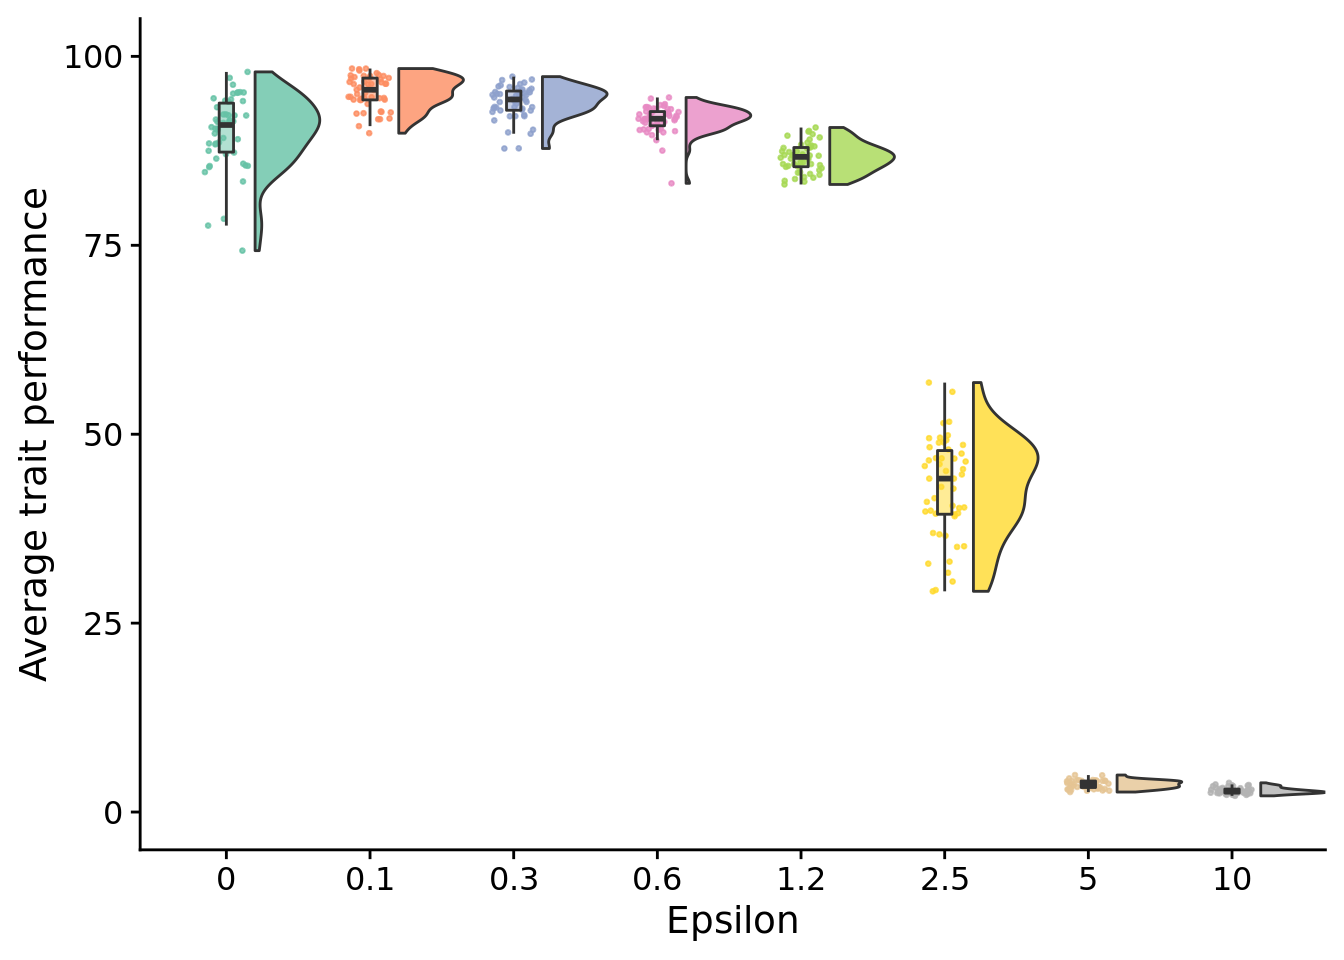
\includegraphics{supplemental-material_files/figure-latex/unnamed-chunk-46-1.pdf}

\hypertarget{unique-starting-positions-3}{%
\section{Unique starting positions}\label{unique-starting-positions-3}}

\begin{Shaded}
\begin{Highlighting}[]
\NormalTok{unique_start_position_coverage_fig <-}\StringTok{ }\KeywordTok{ggplot}\NormalTok{(}
\NormalTok{    data,}
    \KeywordTok{aes}\NormalTok{(}
      \DataTypeTok{x=}\NormalTok{gen,}
      \DataTypeTok{y=}\NormalTok{unique_start_positions_coverage,}
      \DataTypeTok{color=}\NormalTok{epsilon,}
      \DataTypeTok{fill=}\NormalTok{epsilon}
\NormalTok{    )}
\NormalTok{  ) }\OperatorTok{+}
\StringTok{  }\KeywordTok{stat_summary}\NormalTok{(}\DataTypeTok{geom=}\StringTok{"line"}\NormalTok{, }\DataTypeTok{fun=}\NormalTok{mean) }\OperatorTok{+}
\StringTok{  }\KeywordTok{stat_summary}\NormalTok{(}
    \DataTypeTok{geom=}\StringTok{"ribbon"}\NormalTok{,}
    \DataTypeTok{fun.data=}\StringTok{"mean_cl_boot"}\NormalTok{,}
    \DataTypeTok{fun.args=}\KeywordTok{list}\NormalTok{(}\DataTypeTok{conf.int=}\FloatTok{0.95}\NormalTok{),}
    \DataTypeTok{alpha=}\FloatTok{0.2}\NormalTok{,}
    \DataTypeTok{linetype=}\DecValTok{0}
\NormalTok{  ) }\OperatorTok{+}
\StringTok{  }\KeywordTok{scale_y_continuous}\NormalTok{(}
    \DataTypeTok{name=}\StringTok{"Activation position coverage"}\NormalTok{,}
    \DataTypeTok{limits=}\KeywordTok{c}\NormalTok{(}\FloatTok{0.0}\NormalTok{, }\FloatTok{1.0}\NormalTok{)}
\NormalTok{  ) }\OperatorTok{+}
\StringTok{  }\KeywordTok{scale_x_continuous}\NormalTok{(}
    \DataTypeTok{name=}\StringTok{"Generations"}
\NormalTok{  ) }\OperatorTok{+}
\StringTok{  }\KeywordTok{scale_fill_brewer}\NormalTok{(}
    \DataTypeTok{name=}\StringTok{"Epsilon"}\NormalTok{,}
    \DataTypeTok{palette=}\NormalTok{cb_palette}
\NormalTok{  ) }\OperatorTok{+}
\StringTok{  }\KeywordTok{scale_color_brewer}\NormalTok{(}
    \DataTypeTok{name=}\StringTok{"Epsilon"}\NormalTok{,}
    \DataTypeTok{palette=}\NormalTok{cb_palette}
\NormalTok{  )}
\NormalTok{unique_start_position_coverage_fig}
\end{Highlighting}
\end{Shaded}

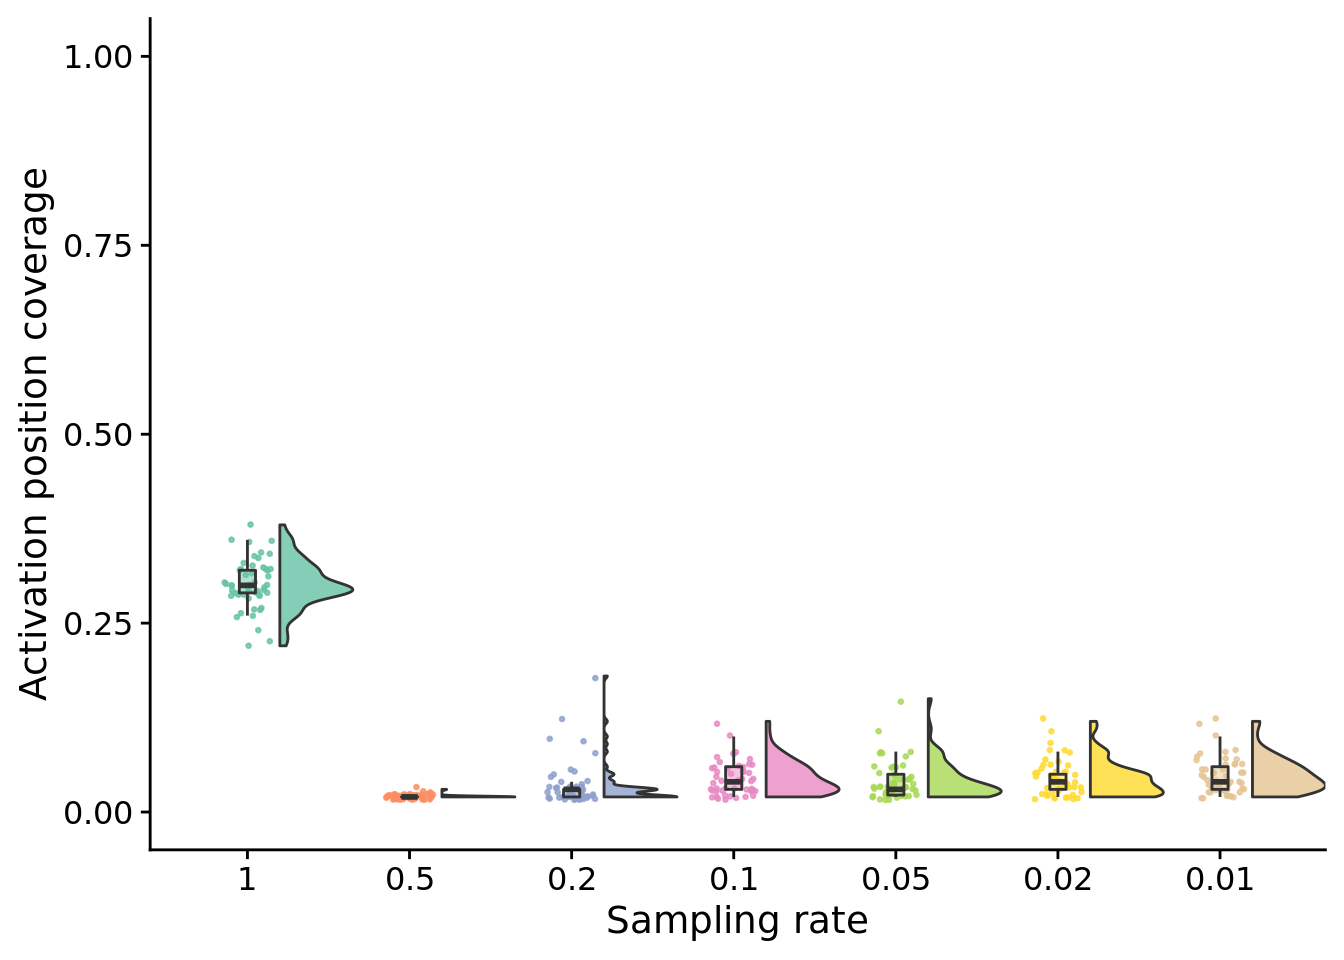
\includegraphics{supplemental-material_files/figure-latex/unnamed-chunk-47-1.pdf}

\hypertarget{final-coverage}{%
\subsection{Final coverage}\label{final-coverage}}

\begin{Shaded}
\begin{Highlighting}[]
\NormalTok{unique_start_positions_coverage_final_fig <-}\StringTok{ }\KeywordTok{ggplot}\NormalTok{(}
\NormalTok{    final_data,}
    \KeywordTok{aes}\NormalTok{(}
      \DataTypeTok{x=}\NormalTok{epsilon,}
      \DataTypeTok{y=}\NormalTok{unique_start_positions_coverage,}
      \DataTypeTok{fill=}\NormalTok{epsilon}
\NormalTok{    )}
\NormalTok{  ) }\OperatorTok{+}
\StringTok{  }\KeywordTok{geom_flat_violin}\NormalTok{(}
    \DataTypeTok{position =} \KeywordTok{position_nudge}\NormalTok{(}\DataTypeTok{x =} \FloatTok{.2}\NormalTok{, }\DataTypeTok{y =} \DecValTok{0}\NormalTok{),}
    \DataTypeTok{alpha =} \FloatTok{.8}\NormalTok{,}
    \DataTypeTok{scale=}\StringTok{"width"}
\NormalTok{  ) }\OperatorTok{+}
\StringTok{  }\KeywordTok{geom_point}\NormalTok{(}
    \DataTypeTok{mapping=}\KeywordTok{aes}\NormalTok{(}\DataTypeTok{color=}\NormalTok{epsilon),}
    \DataTypeTok{position =} \KeywordTok{position_jitter}\NormalTok{(}\DataTypeTok{width =} \FloatTok{.15}\NormalTok{),}
    \DataTypeTok{size =} \FloatTok{.5}\NormalTok{,}
    \DataTypeTok{alpha =} \FloatTok{0.8}
\NormalTok{  ) }\OperatorTok{+}
\StringTok{  }\KeywordTok{geom_boxplot}\NormalTok{(}
    \DataTypeTok{width =} \FloatTok{.1}\NormalTok{,}
    \DataTypeTok{outlier.shape =} \OtherTok{NA}\NormalTok{,}
    \DataTypeTok{alpha =} \FloatTok{0.5}
\NormalTok{  ) }\OperatorTok{+}
\StringTok{  }\KeywordTok{scale_y_continuous}\NormalTok{(}
    \DataTypeTok{name=}\StringTok{"Activation position coverage"}\NormalTok{,}
    \DataTypeTok{limits=}\KeywordTok{c}\NormalTok{(}\DecValTok{0}\NormalTok{, }\FloatTok{1.0}\NormalTok{)}
\NormalTok{  ) }\OperatorTok{+}
\StringTok{  }\KeywordTok{scale_x_discrete}\NormalTok{(}
    \DataTypeTok{name=}\StringTok{"Epsilon"}
\NormalTok{  ) }\OperatorTok{+}
\StringTok{  }\KeywordTok{scale_fill_brewer}\NormalTok{(}
    \DataTypeTok{name=}\StringTok{"Epsilon"}\NormalTok{,}
    \DataTypeTok{palette=}\NormalTok{cb_palette}
\NormalTok{  ) }\OperatorTok{+}
\StringTok{  }\KeywordTok{scale_color_brewer}\NormalTok{(}
    \DataTypeTok{name=}\StringTok{"Epsilon"}\NormalTok{,}
    \DataTypeTok{palette=}\NormalTok{cb_palette}
\NormalTok{  ) }\OperatorTok{+}
\StringTok{  }\KeywordTok{theme}\NormalTok{(}
    \DataTypeTok{legend.position=}\StringTok{"none"}
\NormalTok{  )}
\NormalTok{unique_start_positions_coverage_final_fig}
\end{Highlighting}
\end{Shaded}

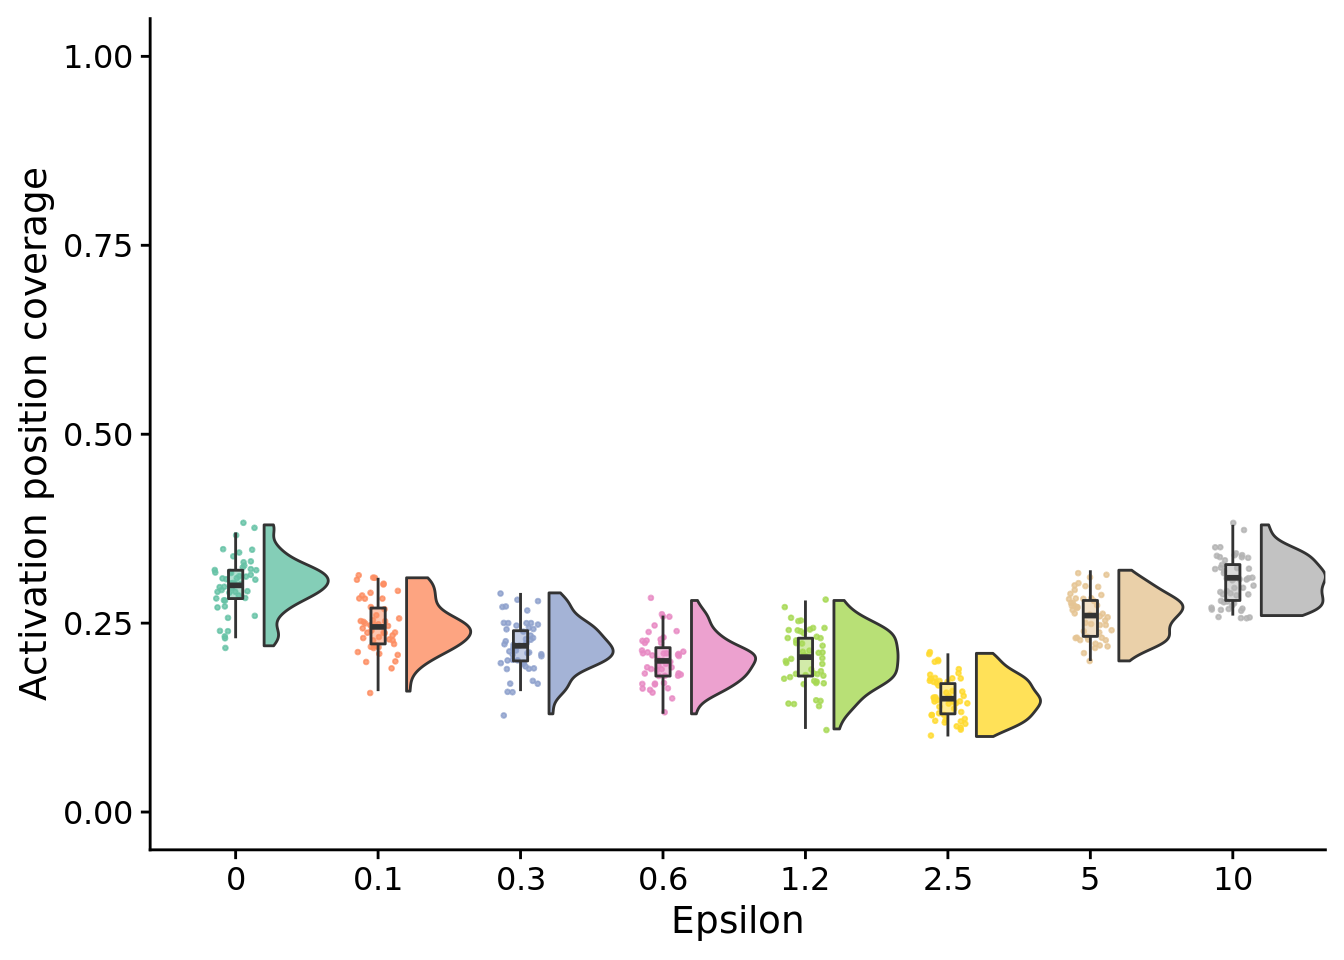
\includegraphics{supplemental-material_files/figure-latex/unnamed-chunk-48-1.pdf}

\hypertarget{manuscript-figures-3}{%
\section{Manuscript figures}\label{manuscript-figures-3}}

\begin{Shaded}
\begin{Highlighting}[]
\NormalTok{legend <-}\StringTok{ }\NormalTok{cowplot}\OperatorTok{::}\KeywordTok{get_legend}\NormalTok{(}
\NormalTok{    elite_ave_performance_fig }\OperatorTok{+}
\StringTok{      }\KeywordTok{guides}\NormalTok{(}
        \DataTypeTok{color=}\KeywordTok{guide_legend}\NormalTok{(}\DataTypeTok{nrow=}\DecValTok{1}\NormalTok{),}
        \DataTypeTok{fill=}\KeywordTok{guide_legend}\NormalTok{(}\DataTypeTok{nrow=}\DecValTok{1}\NormalTok{)}
\NormalTok{      ) }\OperatorTok{+}
\StringTok{      }\KeywordTok{theme}\NormalTok{(}
        \DataTypeTok{legend.position =} \StringTok{"bottom"}\NormalTok{,}
        \DataTypeTok{legend.box=}\StringTok{"horizontal"}\NormalTok{,}
        \DataTypeTok{legend.justification=}\StringTok{"center"}
\NormalTok{      )}
\NormalTok{  )}

\NormalTok{grid <-}\StringTok{ }\KeywordTok{plot_grid}\NormalTok{(}
\NormalTok{  elite_ave_performance_fig }\OperatorTok{+}
\StringTok{    }\KeywordTok{ggtitle}\NormalTok{(}\StringTok{"Performance over time"}\NormalTok{) }\OperatorTok{+}
\StringTok{    }\KeywordTok{theme}\NormalTok{(}\DataTypeTok{legend.position=}\StringTok{"none"}\NormalTok{),}
\NormalTok{  elite_final_performance_fig }\OperatorTok{+}
\StringTok{    }\KeywordTok{ggtitle}\NormalTok{(}\StringTok{"Final performance"}\NormalTok{) }\OperatorTok{+}
\StringTok{    }\KeywordTok{theme}\NormalTok{(),}
\NormalTok{  unique_start_position_coverage_fig }\OperatorTok{+}
\StringTok{    }\KeywordTok{ggtitle}\NormalTok{(}\StringTok{"Activation position coverage over time"}\NormalTok{) }\OperatorTok{+}
\StringTok{    }\KeywordTok{theme}\NormalTok{(}\DataTypeTok{legend.position=}\StringTok{"none"}\NormalTok{),}
\NormalTok{  unique_start_positions_coverage_final_fig }\OperatorTok{+}
\StringTok{    }\KeywordTok{ggtitle}\NormalTok{(}\StringTok{"Final activation position coverage"}\NormalTok{) }\OperatorTok{+}
\StringTok{    }\KeywordTok{theme}\NormalTok{(),}
  \DataTypeTok{nrow=}\DecValTok{2}\NormalTok{,}
  \DataTypeTok{ncol=}\DecValTok{2}\NormalTok{,}
  \DataTypeTok{rel_widths=}\KeywordTok{c}\NormalTok{(}\DecValTok{3}\NormalTok{,}\DecValTok{2}\NormalTok{),}
  \DataTypeTok{labels=}\StringTok{"auto"}
\NormalTok{)}

\NormalTok{grid <-}\StringTok{ }\KeywordTok{plot_grid}\NormalTok{(}
\NormalTok{  grid,}
\NormalTok{  legend,}
  \DataTypeTok{nrow=}\DecValTok{2}\NormalTok{,}
  \DataTypeTok{ncol=}\DecValTok{1}\NormalTok{,}
  \DataTypeTok{rel_heights=}\KeywordTok{c}\NormalTok{(}\DecValTok{1}\NormalTok{, }\FloatTok{0.1}\NormalTok{)}
\NormalTok{)}

\KeywordTok{save_plot}\NormalTok{(}
  \KeywordTok{paste}\NormalTok{(working_directory, }\StringTok{"imgs/epsilon-panel.pdf"}\NormalTok{, }\DataTypeTok{sep=}\StringTok{""}\NormalTok{),}
\NormalTok{  grid,}
  \DataTypeTok{base_width=}\DecValTok{12}\NormalTok{,}
  \DataTypeTok{base_height=}\DecValTok{8}
\NormalTok{)}

\NormalTok{grid}
\end{Highlighting}
\end{Shaded}

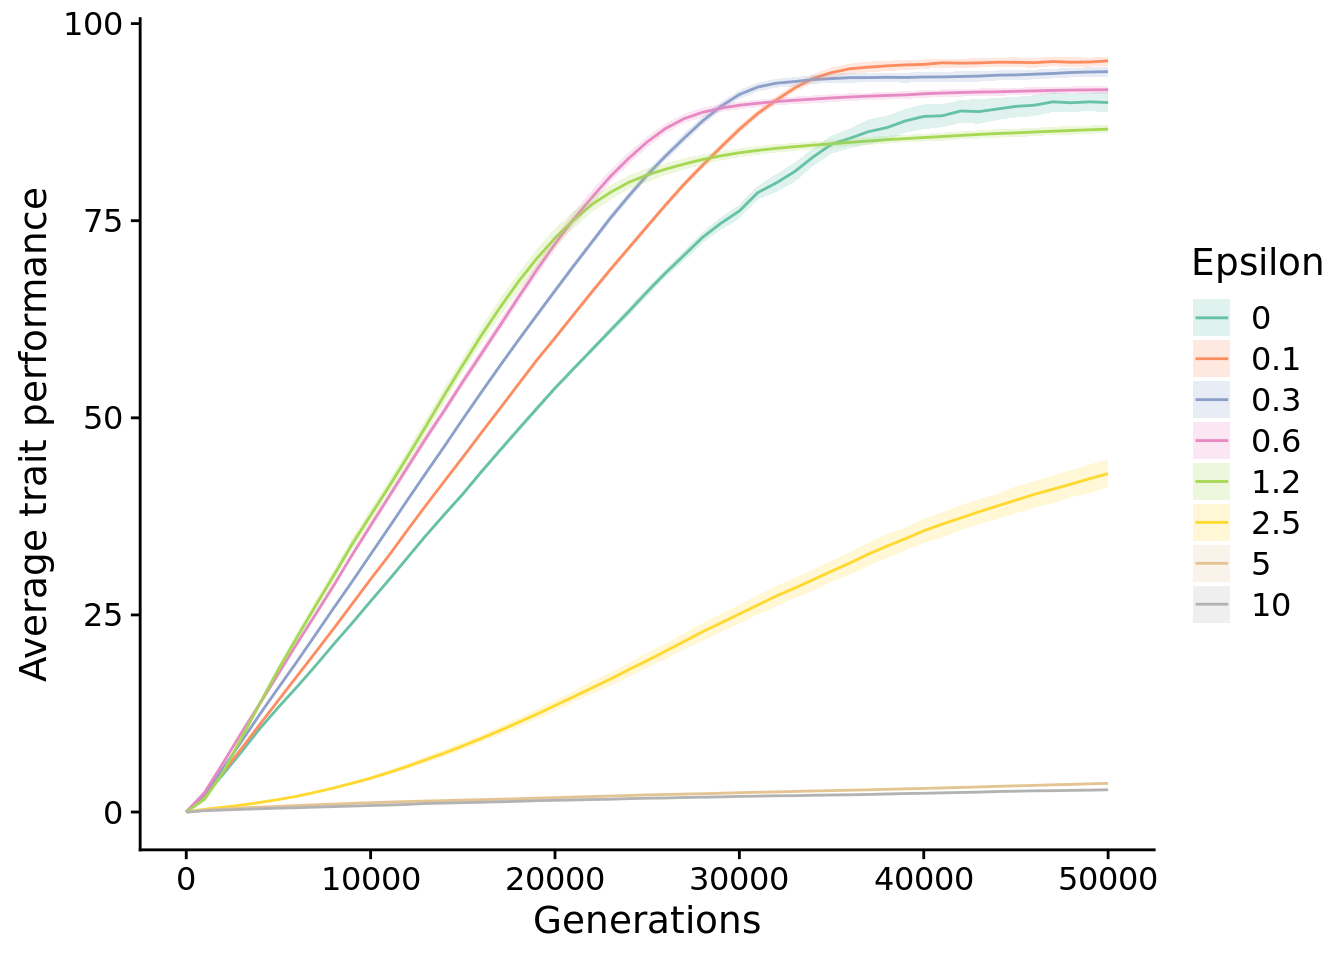
\includegraphics{supplemental-material_files/figure-latex/unnamed-chunk-49-1.pdf}

\hypertarget{down-sampled-lexicase}{%
\chapter{Down-sampled lexicase}\label{down-sampled-lexicase}}

\hypertarget{overview-4}{%
\section{Overview}\label{overview-4}}

\begin{Shaded}
\begin{Highlighting}[]
\CommentTok{# Relative location of data.}
\NormalTok{working_directory <-}\StringTok{ "experiments/2021-05-28-downsampled/analysis/"}
\CommentTok{# working_directory <- "./"}

\CommentTok{# Settings for visualization}
\NormalTok{cb_palette <-}\StringTok{ "Set2"}
\CommentTok{# Create directory to dump plots}
\KeywordTok{dir.create}\NormalTok{(}\KeywordTok{paste0}\NormalTok{(working_directory, }\StringTok{"imgs"}\NormalTok{), }\DataTypeTok{showWarnings=}\OtherTok{FALSE}\NormalTok{)}
\end{Highlighting}
\end{Shaded}

\hypertarget{analysis-dependencies-4}{%
\section{Analysis dependencies}\label{analysis-dependencies-4}}

\begin{Shaded}
\begin{Highlighting}[]
\KeywordTok{library}\NormalTok{(ggplot2)}
\KeywordTok{library}\NormalTok{(tidyverse)}
\KeywordTok{library}\NormalTok{(cowplot)}
\KeywordTok{library}\NormalTok{(viridis)}
\KeywordTok{library}\NormalTok{(RColorBrewer)}
\KeywordTok{source}\NormalTok{(}\StringTok{"https://gist.githubusercontent.com/benmarwick/2a1bb0133ff568cbe28d/raw/fb53bd97121f7f9ce947837ef1a4c65a73bffb3f/geom_flat_violin.R"}\NormalTok{)}
\end{Highlighting}
\end{Shaded}

These analyses were conducted in the following computing environment:

\begin{Shaded}
\begin{Highlighting}[]
\KeywordTok{print}\NormalTok{(version)}
\end{Highlighting}
\end{Shaded}

\begin{verbatim}
##                _                           
## platform       x86_64-pc-linux-gnu         
## arch           x86_64                      
## os             linux-gnu                   
## system         x86_64, linux-gnu           
## status                                     
## major          4                           
## minor          1.0                         
## year           2021                        
## month          05                          
## day            18                          
## svn rev        80317                       
## language       R                           
## version.string R version 4.1.0 (2021-05-18)
## nickname       Camp Pontanezen
\end{verbatim}

\hypertarget{setup-4}{%
\section{Setup}\label{setup-4}}

\begin{Shaded}
\begin{Highlighting}[]
\NormalTok{data_loc <-}\StringTok{ }\KeywordTok{paste0}\NormalTok{(working_directory, }\StringTok{"data/timeseries.csv"}\NormalTok{)}
\NormalTok{data <-}\StringTok{ }\KeywordTok{read.csv}\NormalTok{(data_loc, }\DataTypeTok{na.strings=}\StringTok{"NONE"}\NormalTok{)}

\NormalTok{data}\OperatorTok{$}\NormalTok{cardinality <-}\StringTok{ }\KeywordTok{as.factor}\NormalTok{(}
\NormalTok{  data}\OperatorTok{$}\NormalTok{OBJECTIVE_CNT}
\NormalTok{)}
\NormalTok{data}\OperatorTok{$}\NormalTok{selection_name <-}\StringTok{ }\KeywordTok{as.factor}\NormalTok{(}
\NormalTok{  data}\OperatorTok{$}\NormalTok{selection_name}
\NormalTok{)}

\NormalTok{data}\OperatorTok{$}\NormalTok{epsilon <-}\StringTok{ }\KeywordTok{as.factor}\NormalTok{(}
\NormalTok{  data}\OperatorTok{$}\NormalTok{LEX_EPS}
\NormalTok{)}

\NormalTok{data}\OperatorTok{$}\NormalTok{proportion <-}\StringTok{ }\KeywordTok{factor}\NormalTok{(}
\NormalTok{  data}\OperatorTok{$}\NormalTok{DSLEX_PROP,}
  \DataTypeTok{levels=}\KeywordTok{c}\NormalTok{(}\DecValTok{1}\NormalTok{, }\FloatTok{0.5}\NormalTok{, }\FloatTok{0.2}\NormalTok{, }\FloatTok{0.1}\NormalTok{, }\FloatTok{0.05}\NormalTok{, }\FloatTok{0.02}\NormalTok{, }\FloatTok{0.01}\NormalTok{)}
\NormalTok{)}

\NormalTok{data}\OperatorTok{$}\NormalTok{elite_trait_avg <-}\StringTok{ }\NormalTok{data}\OperatorTok{$}\NormalTok{ele_agg_per }\OperatorTok{/}\StringTok{ }\NormalTok{data}\OperatorTok{$}\NormalTok{OBJECTIVE_CNT}
\NormalTok{data}\OperatorTok{$}\NormalTok{unique_start_positions_coverage <-}\StringTok{ }\NormalTok{data}\OperatorTok{$}\NormalTok{uni_str_pos }\OperatorTok{/}\StringTok{ }\NormalTok{data}\OperatorTok{$}\NormalTok{OBJECTIVE_CNT}

\NormalTok{final_data <-}\StringTok{ }\KeywordTok{filter}\NormalTok{(data, evaluations}\OperatorTok{==}\KeywordTok{max}\NormalTok{(data}\OperatorTok{$}\NormalTok{evaluations))}

\CommentTok{####### misc #######}
\CommentTok{# Configure our default graphing theme}
\KeywordTok{theme_set}\NormalTok{(}\KeywordTok{theme_cowplot}\NormalTok{())}
\end{Highlighting}
\end{Shaded}

\hypertarget{exploration-diagnostic-performance-4}{%
\section{Exploration diagnostic performance}\label{exploration-diagnostic-performance-4}}

\begin{Shaded}
\begin{Highlighting}[]
\NormalTok{elite_ave_performance_fig <-}
\StringTok{  }\KeywordTok{ggplot}\NormalTok{(}
\NormalTok{    data,}
    \KeywordTok{aes}\NormalTok{(}
      \DataTypeTok{x=}\NormalTok{evaluations,}
      \DataTypeTok{y=}\NormalTok{elite_trait_avg,}
      \DataTypeTok{color=}\NormalTok{proportion,}
      \DataTypeTok{fill=}\NormalTok{proportion}
\NormalTok{    )}
\NormalTok{  ) }\OperatorTok{+}
\StringTok{  }\KeywordTok{stat_summary}\NormalTok{(}\DataTypeTok{geom=}\StringTok{"line"}\NormalTok{, }\DataTypeTok{fun=}\NormalTok{mean) }\OperatorTok{+}
\StringTok{  }\KeywordTok{stat_summary}\NormalTok{(}
    \DataTypeTok{geom=}\StringTok{"ribbon"}\NormalTok{,}
    \DataTypeTok{fun.data=}\StringTok{"mean_cl_boot"}\NormalTok{,}
    \DataTypeTok{fun.args=}\KeywordTok{list}\NormalTok{(}\DataTypeTok{conf.int=}\FloatTok{0.95}\NormalTok{),}
    \DataTypeTok{alpha=}\FloatTok{0.2}\NormalTok{,}
    \DataTypeTok{linetype=}\DecValTok{0}
\NormalTok{  ) }\OperatorTok{+}
\StringTok{  }\KeywordTok{scale_y_continuous}\NormalTok{(}
    \DataTypeTok{name=}\StringTok{"Average trait performance"}\NormalTok{,}
    \DataTypeTok{limits=}\KeywordTok{c}\NormalTok{(}\DecValTok{0}\NormalTok{, }\DecValTok{100}\NormalTok{)}
\NormalTok{  ) }\OperatorTok{+}
\StringTok{  }\KeywordTok{scale_x_continuous}\NormalTok{(}
    \DataTypeTok{name=}\StringTok{"Evaluations"}
\NormalTok{  ) }\OperatorTok{+}
\StringTok{  }\KeywordTok{scale_fill_brewer}\NormalTok{(}
    \DataTypeTok{name=}\StringTok{"Sampling rate"}\NormalTok{,}
    \DataTypeTok{palette=}\NormalTok{cb_palette}
\NormalTok{  ) }\OperatorTok{+}
\StringTok{  }\KeywordTok{scale_color_brewer}\NormalTok{(}
    \DataTypeTok{name=}\StringTok{"Sampling rate"}\NormalTok{,}
    \DataTypeTok{palette=}\NormalTok{cb_palette}
\NormalTok{  )}
\NormalTok{elite_ave_performance_fig}
\end{Highlighting}
\end{Shaded}

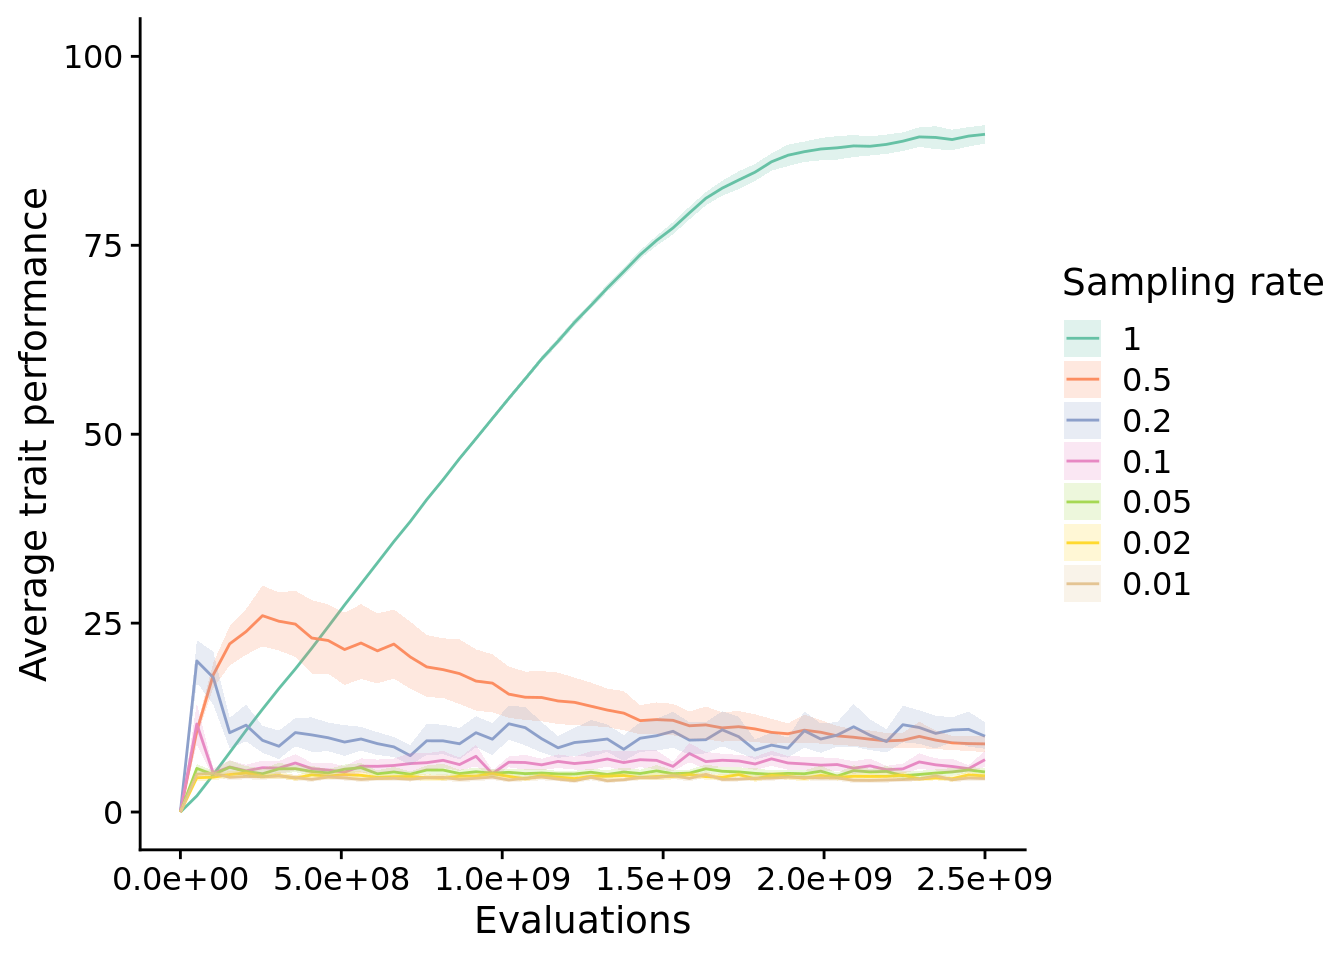
\includegraphics{supplemental-material_files/figure-latex/unnamed-chunk-54-1.pdf}

\hypertarget{final-performance-4}{%
\subsection{Final performance}\label{final-performance-4}}

\begin{Shaded}
\begin{Highlighting}[]
\NormalTok{elite_final_performance_fig <-}\StringTok{ }\KeywordTok{ggplot}\NormalTok{(}
\NormalTok{    final_data,}
    \KeywordTok{aes}\NormalTok{(}
      \DataTypeTok{x=}\NormalTok{proportion,}
      \DataTypeTok{y=}\NormalTok{elite_trait_avg,}
      \DataTypeTok{fill=}\NormalTok{proportion}
\NormalTok{    )}
\NormalTok{  ) }\OperatorTok{+}
\StringTok{  }\KeywordTok{geom_flat_violin}\NormalTok{(}
    \DataTypeTok{position =} \KeywordTok{position_nudge}\NormalTok{(}\DataTypeTok{x =} \FloatTok{.2}\NormalTok{, }\DataTypeTok{y =} \DecValTok{0}\NormalTok{),}
    \DataTypeTok{alpha =} \FloatTok{.8}\NormalTok{,}
    \DataTypeTok{scale=}\StringTok{"width"}
\NormalTok{  ) }\OperatorTok{+}
\StringTok{  }\KeywordTok{geom_point}\NormalTok{(}
    \DataTypeTok{mapping=}\KeywordTok{aes}\NormalTok{(}\DataTypeTok{color=}\NormalTok{proportion),}
    \DataTypeTok{position =} \KeywordTok{position_jitter}\NormalTok{(}\DataTypeTok{width =} \FloatTok{.15}\NormalTok{),}
    \DataTypeTok{size =} \FloatTok{.5}\NormalTok{,}
    \DataTypeTok{alpha =} \FloatTok{0.8}
\NormalTok{  ) }\OperatorTok{+}
\StringTok{  }\KeywordTok{geom_boxplot}\NormalTok{(}
    \DataTypeTok{width =} \FloatTok{.1}\NormalTok{,}
    \DataTypeTok{outlier.shape =} \OtherTok{NA}\NormalTok{,}
    \DataTypeTok{alpha =} \FloatTok{0.5}
\NormalTok{  ) }\OperatorTok{+}
\StringTok{  }\KeywordTok{scale_y_continuous}\NormalTok{(}
    \DataTypeTok{name=}\StringTok{"Average trait performance"}\NormalTok{,}
    \DataTypeTok{limits=}\KeywordTok{c}\NormalTok{(}\DecValTok{0}\NormalTok{, }\DecValTok{100}\NormalTok{)}
\NormalTok{  ) }\OperatorTok{+}
\StringTok{  }\KeywordTok{scale_x_discrete}\NormalTok{(}
    \DataTypeTok{name=}\StringTok{"Sampling rate"}
\NormalTok{  ) }\OperatorTok{+}
\StringTok{  }\KeywordTok{scale_fill_brewer}\NormalTok{(}
    \DataTypeTok{name=}\StringTok{"Sampling rate"}\NormalTok{,}
    \DataTypeTok{palette=}\NormalTok{cb_palette}
\NormalTok{  ) }\OperatorTok{+}
\StringTok{  }\KeywordTok{scale_color_brewer}\NormalTok{(}
    \DataTypeTok{name=}\StringTok{"Sampling rate"}\NormalTok{,}
    \DataTypeTok{palette=}\NormalTok{cb_palette}
\NormalTok{  ) }\OperatorTok{+}
\StringTok{  }\KeywordTok{theme}\NormalTok{(}
    \DataTypeTok{legend.position=}\StringTok{"none"}
\NormalTok{  )}
\NormalTok{elite_final_performance_fig}
\end{Highlighting}
\end{Shaded}

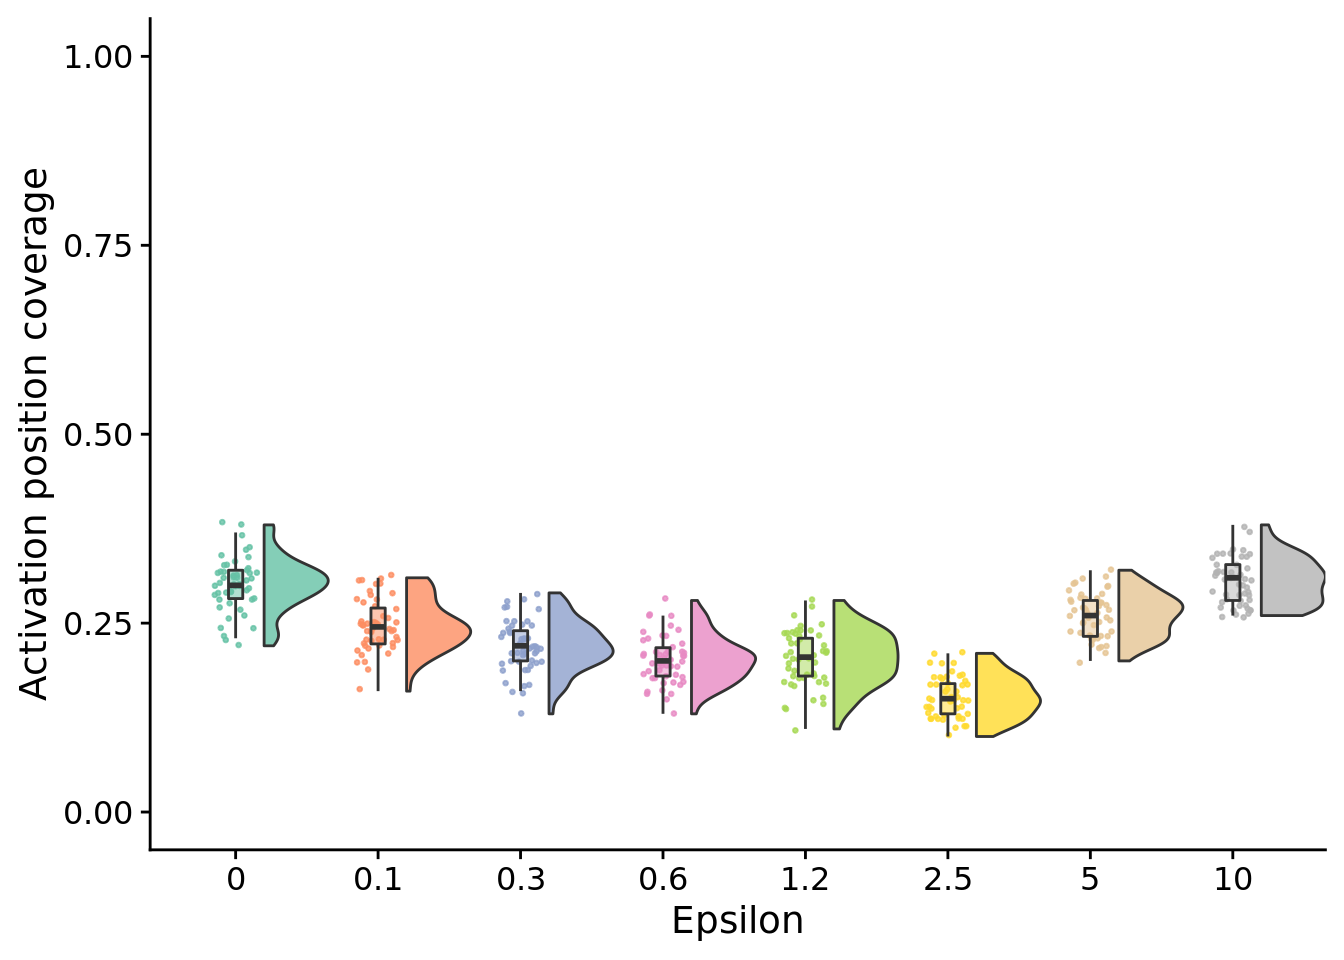
\includegraphics{supplemental-material_files/figure-latex/unnamed-chunk-55-1.pdf}

\hypertarget{unique-starting-positions-4}{%
\section{Unique starting positions}\label{unique-starting-positions-4}}

\begin{Shaded}
\begin{Highlighting}[]
\NormalTok{unique_start_position_coverage_fig <-}\StringTok{ }\KeywordTok{ggplot}\NormalTok{(}
\NormalTok{    data,}
    \KeywordTok{aes}\NormalTok{(}
      \DataTypeTok{x=}\NormalTok{evaluations,}
      \DataTypeTok{y=}\NormalTok{unique_start_positions_coverage,}
      \DataTypeTok{color=}\NormalTok{proportion,}
      \DataTypeTok{fill=}\NormalTok{proportion}
\NormalTok{    )}
\NormalTok{  ) }\OperatorTok{+}
\StringTok{  }\KeywordTok{stat_summary}\NormalTok{(}\DataTypeTok{geom=}\StringTok{"line"}\NormalTok{, }\DataTypeTok{fun=}\NormalTok{mean) }\OperatorTok{+}
\StringTok{  }\KeywordTok{stat_summary}\NormalTok{(}
    \DataTypeTok{geom=}\StringTok{"ribbon"}\NormalTok{,}
    \DataTypeTok{fun.data=}\StringTok{"mean_cl_boot"}\NormalTok{,}
    \DataTypeTok{fun.args=}\KeywordTok{list}\NormalTok{(}\DataTypeTok{conf.int=}\FloatTok{0.95}\NormalTok{),}
    \DataTypeTok{alpha=}\FloatTok{0.2}\NormalTok{,}
    \DataTypeTok{linetype=}\DecValTok{0}
\NormalTok{  ) }\OperatorTok{+}
\StringTok{  }\KeywordTok{scale_y_continuous}\NormalTok{(}
    \DataTypeTok{name=}\StringTok{"Activation position coverage"}\NormalTok{,}
    \DataTypeTok{limits=}\KeywordTok{c}\NormalTok{(}\FloatTok{0.0}\NormalTok{, }\FloatTok{1.0}\NormalTok{)}
\NormalTok{  ) }\OperatorTok{+}
\StringTok{  }\KeywordTok{scale_x_continuous}\NormalTok{(}
    \DataTypeTok{name=}\StringTok{"Evaluations"}
\NormalTok{  ) }\OperatorTok{+}
\StringTok{  }\KeywordTok{scale_fill_brewer}\NormalTok{(}
    \DataTypeTok{name=}\StringTok{"Sampling rate"}\NormalTok{,}
    \DataTypeTok{palette=}\NormalTok{cb_palette}
\NormalTok{  ) }\OperatorTok{+}
\StringTok{  }\KeywordTok{scale_color_brewer}\NormalTok{(}
    \DataTypeTok{name=}\StringTok{"Sampling rate"}\NormalTok{,}
    \DataTypeTok{palette=}\NormalTok{cb_palette}
\NormalTok{  )}
\NormalTok{unique_start_position_coverage_fig}
\end{Highlighting}
\end{Shaded}

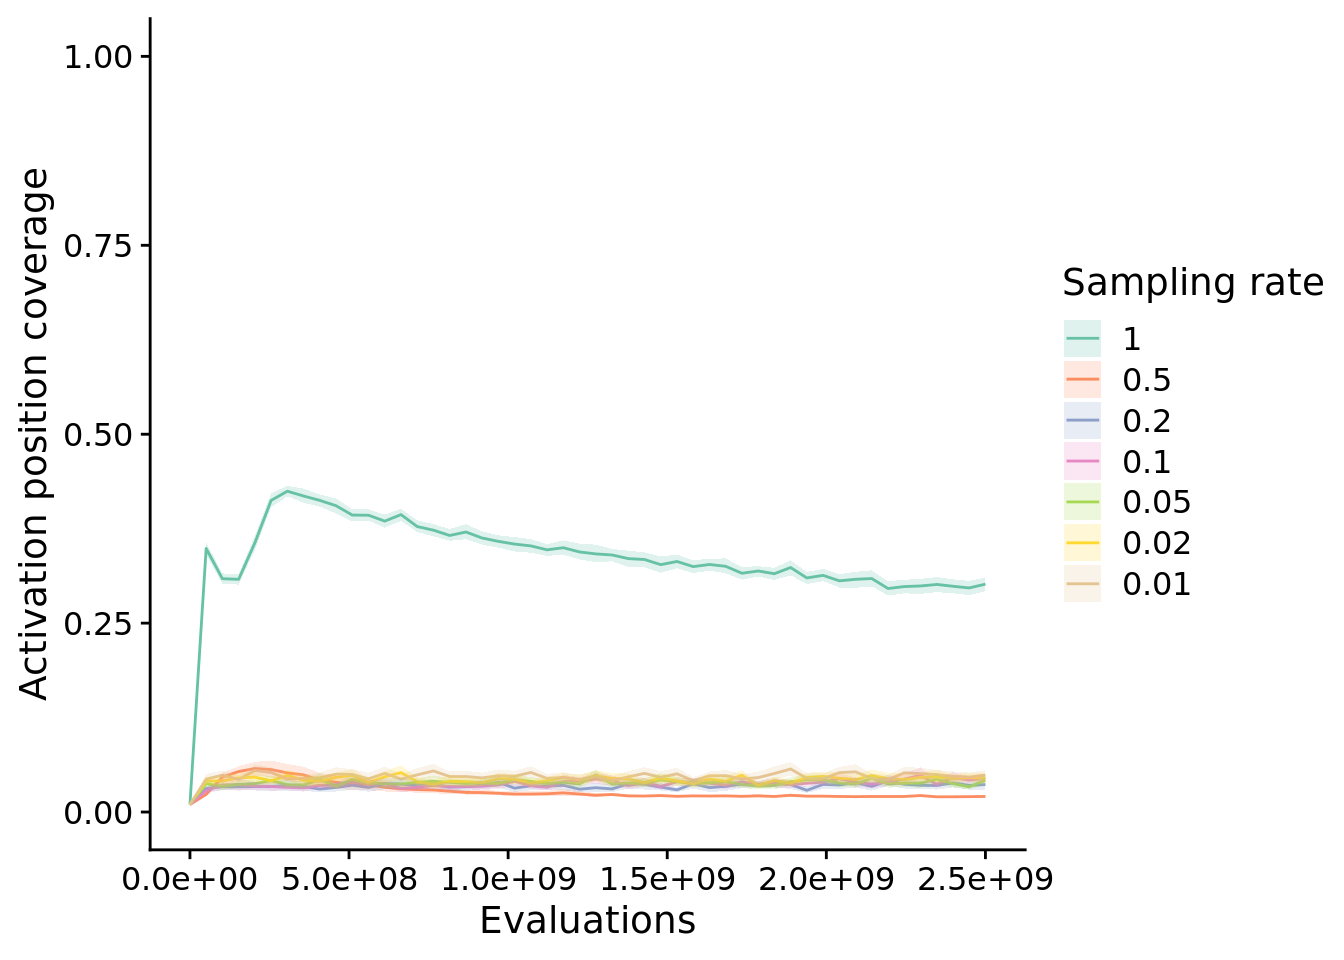
\includegraphics{supplemental-material_files/figure-latex/unnamed-chunk-56-1.pdf}

\hypertarget{final-starting-position-coverage-3}{%
\subsection{Final starting position coverage}\label{final-starting-position-coverage-3}}

\begin{Shaded}
\begin{Highlighting}[]
\NormalTok{unique_start_positions_coverage_final_fig <-}\StringTok{ }\KeywordTok{ggplot}\NormalTok{(}
\NormalTok{    final_data,}
    \KeywordTok{aes}\NormalTok{(}
      \DataTypeTok{x=}\NormalTok{proportion,}
      \DataTypeTok{y=}\NormalTok{unique_start_positions_coverage,}
      \DataTypeTok{fill=}\NormalTok{proportion}
\NormalTok{    )}
\NormalTok{  ) }\OperatorTok{+}
\StringTok{  }\KeywordTok{geom_flat_violin}\NormalTok{(}
    \DataTypeTok{position =} \KeywordTok{position_nudge}\NormalTok{(}\DataTypeTok{x =} \FloatTok{.2}\NormalTok{, }\DataTypeTok{y =} \DecValTok{0}\NormalTok{),}
    \DataTypeTok{alpha =} \FloatTok{.8}\NormalTok{,}
    \DataTypeTok{scale=}\StringTok{"width"}
\NormalTok{  ) }\OperatorTok{+}
\StringTok{  }\KeywordTok{geom_point}\NormalTok{(}
    \DataTypeTok{mapping=}\KeywordTok{aes}\NormalTok{(}\DataTypeTok{color=}\NormalTok{proportion),}
    \DataTypeTok{position =} \KeywordTok{position_jitter}\NormalTok{(}\DataTypeTok{width =} \FloatTok{.15}\NormalTok{),}
    \DataTypeTok{size =} \FloatTok{.5}\NormalTok{,}
    \DataTypeTok{alpha =} \FloatTok{0.8}
\NormalTok{  ) }\OperatorTok{+}
\StringTok{  }\KeywordTok{geom_boxplot}\NormalTok{(}
    \DataTypeTok{width =} \FloatTok{.1}\NormalTok{,}
    \DataTypeTok{outlier.shape =} \OtherTok{NA}\NormalTok{,}
    \DataTypeTok{alpha =} \FloatTok{0.5}
\NormalTok{  ) }\OperatorTok{+}
\StringTok{  }\KeywordTok{scale_y_continuous}\NormalTok{(}
    \DataTypeTok{name=}\StringTok{"Activation position coverage"}\NormalTok{,}
    \DataTypeTok{limits=}\KeywordTok{c}\NormalTok{(}\DecValTok{0}\NormalTok{, }\FloatTok{1.0}\NormalTok{)}
\NormalTok{  ) }\OperatorTok{+}
\StringTok{  }\KeywordTok{scale_x_discrete}\NormalTok{(}
    \DataTypeTok{name=}\StringTok{"Sampling rate"}
\NormalTok{  ) }\OperatorTok{+}
\StringTok{  }\KeywordTok{scale_fill_brewer}\NormalTok{(}
    \DataTypeTok{name=}\StringTok{"Sampling rate"}\NormalTok{,}
    \DataTypeTok{palette=}\NormalTok{cb_palette}
\NormalTok{  ) }\OperatorTok{+}
\StringTok{  }\KeywordTok{scale_color_brewer}\NormalTok{(}
    \DataTypeTok{name=}\StringTok{"Sampling rate"}\NormalTok{,}
    \DataTypeTok{palette=}\NormalTok{cb_palette}
\NormalTok{  ) }\OperatorTok{+}
\StringTok{  }\KeywordTok{theme}\NormalTok{(}
    \DataTypeTok{legend.position=}\StringTok{"none"}
\NormalTok{  )}
\NormalTok{unique_start_positions_coverage_final_fig}
\end{Highlighting}
\end{Shaded}

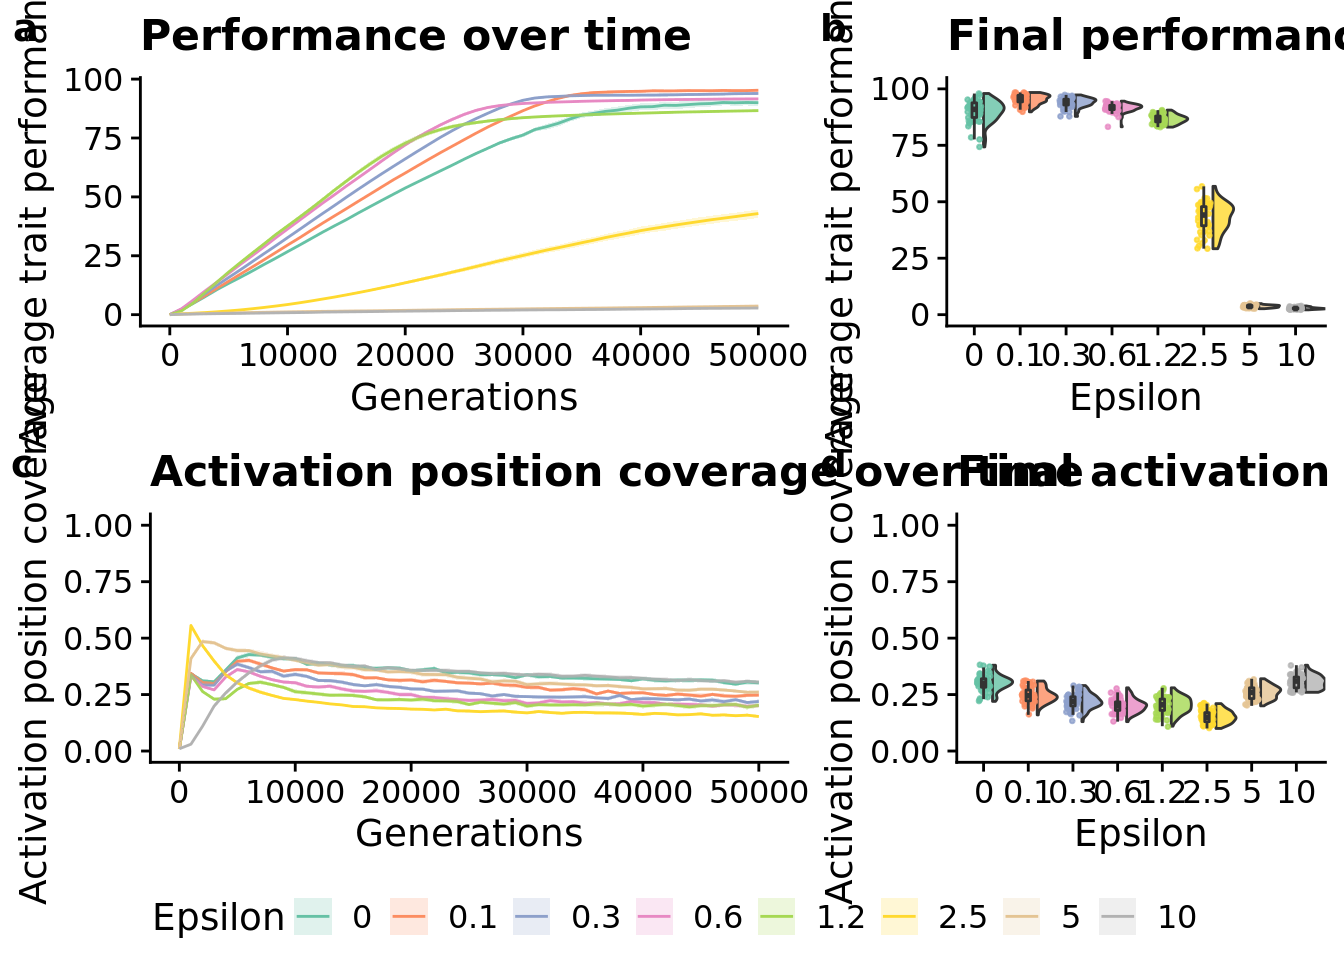
\includegraphics{supplemental-material_files/figure-latex/unnamed-chunk-57-1.pdf}

\hypertarget{manuscript-figures-4}{%
\section{Manuscript figures}\label{manuscript-figures-4}}

\begin{Shaded}
\begin{Highlighting}[]
\NormalTok{legend <-}\StringTok{ }\NormalTok{cowplot}\OperatorTok{::}\KeywordTok{get_legend}\NormalTok{(}
\NormalTok{    elite_ave_performance_fig }\OperatorTok{+}
\StringTok{      }\KeywordTok{guides}\NormalTok{(}
        \DataTypeTok{color=}\KeywordTok{guide_legend}\NormalTok{(}\DataTypeTok{nrow=}\DecValTok{1}\NormalTok{),}
        \DataTypeTok{fill=}\KeywordTok{guide_legend}\NormalTok{(}\DataTypeTok{nrow=}\DecValTok{1}\NormalTok{)}
\NormalTok{      ) }\OperatorTok{+}
\StringTok{      }\KeywordTok{theme}\NormalTok{(}
        \DataTypeTok{legend.position =} \StringTok{"bottom"}\NormalTok{,}
        \DataTypeTok{legend.box=}\StringTok{"horizontal"}\NormalTok{,}
        \DataTypeTok{legend.justification=}\StringTok{"center"}
\NormalTok{      )}
\NormalTok{  )}

\NormalTok{grid <-}\StringTok{ }\KeywordTok{plot_grid}\NormalTok{(}
\NormalTok{  elite_ave_performance_fig }\OperatorTok{+}
\StringTok{    }\KeywordTok{ggtitle}\NormalTok{(}\StringTok{"Performance over time"}\NormalTok{) }\OperatorTok{+}
\StringTok{    }\KeywordTok{theme}\NormalTok{(}\DataTypeTok{legend.position=}\StringTok{"none"}\NormalTok{),}
\NormalTok{  elite_final_performance_fig }\OperatorTok{+}
\StringTok{    }\KeywordTok{ggtitle}\NormalTok{(}\StringTok{"Final performance"}\NormalTok{) }\OperatorTok{+}
\StringTok{    }\KeywordTok{theme}\NormalTok{(),}
\NormalTok{  unique_start_position_coverage_fig }\OperatorTok{+}
\StringTok{    }\KeywordTok{ggtitle}\NormalTok{(}\StringTok{"Activation position coverage over time"}\NormalTok{) }\OperatorTok{+}
\StringTok{    }\KeywordTok{theme}\NormalTok{(}\DataTypeTok{legend.position=}\StringTok{"none"}\NormalTok{),}
\NormalTok{  unique_start_positions_coverage_final_fig }\OperatorTok{+}
\StringTok{    }\KeywordTok{ggtitle}\NormalTok{(}\StringTok{"Final activation position coverage"}\NormalTok{) }\OperatorTok{+}
\StringTok{    }\KeywordTok{theme}\NormalTok{(),}
  \DataTypeTok{nrow=}\DecValTok{2}\NormalTok{,}
  \DataTypeTok{ncol=}\DecValTok{2}\NormalTok{,}
  \DataTypeTok{rel_widths=}\KeywordTok{c}\NormalTok{(}\DecValTok{3}\NormalTok{,}\DecValTok{2}\NormalTok{),}
  \DataTypeTok{labels=}\StringTok{"auto"}
\NormalTok{)}

\NormalTok{grid <-}\StringTok{ }\KeywordTok{plot_grid}\NormalTok{(}
\NormalTok{  grid,}
\NormalTok{  legend,}
  \DataTypeTok{nrow=}\DecValTok{2}\NormalTok{,}
  \DataTypeTok{ncol=}\DecValTok{1}\NormalTok{,}
  \DataTypeTok{rel_heights=}\KeywordTok{c}\NormalTok{(}\DecValTok{1}\NormalTok{, }\FloatTok{0.1}\NormalTok{)}
\NormalTok{)}

\KeywordTok{save_plot}\NormalTok{(}
  \KeywordTok{paste}\NormalTok{(working_directory, }\StringTok{"imgs/down-sampled-panel.pdf"}\NormalTok{, }\DataTypeTok{sep=}\StringTok{""}\NormalTok{),}
\NormalTok{  grid,}
  \DataTypeTok{base_width=}\DecValTok{12}\NormalTok{,}
  \DataTypeTok{base_height=}\DecValTok{8}
\NormalTok{)}

\NormalTok{grid}
\end{Highlighting}
\end{Shaded}

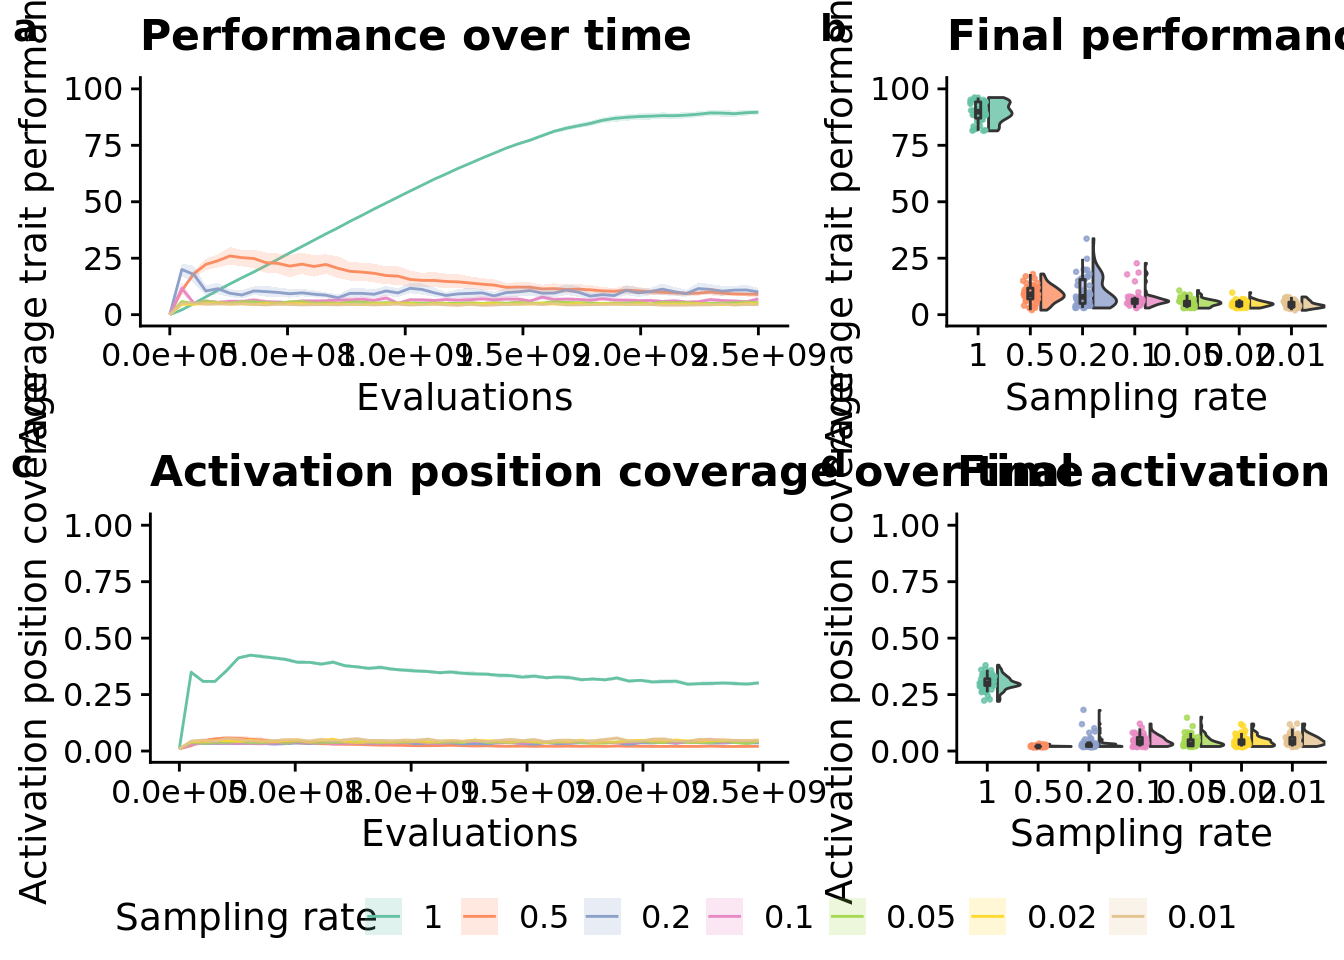
\includegraphics{supplemental-material_files/figure-latex/unnamed-chunk-58-1.pdf}

\hypertarget{cohort-lexicase}{%
\chapter{Cohort lexicase}\label{cohort-lexicase}}

\hypertarget{overview-5}{%
\section{Overview}\label{overview-5}}

\begin{Shaded}
\begin{Highlighting}[]
\CommentTok{# Relative location of data.}
\NormalTok{working_directory <-}\StringTok{ "experiments/2021-06-01-cohort/analysis/"}
\CommentTok{# working_directory <- "./"}

\CommentTok{# Settings for visualization}
\NormalTok{cb_palette <-}\StringTok{ "Set2"}
\CommentTok{# Create directory to dump plots}
\KeywordTok{dir.create}\NormalTok{(}\KeywordTok{paste0}\NormalTok{(working_directory, }\StringTok{"imgs"}\NormalTok{), }\DataTypeTok{showWarnings=}\OtherTok{FALSE}\NormalTok{)}
\end{Highlighting}
\end{Shaded}

\hypertarget{analysis-dependencies-5}{%
\section{Analysis dependencies}\label{analysis-dependencies-5}}

\begin{Shaded}
\begin{Highlighting}[]
\KeywordTok{library}\NormalTok{(ggplot2)}
\KeywordTok{library}\NormalTok{(tidyverse)}
\KeywordTok{library}\NormalTok{(cowplot)}
\KeywordTok{library}\NormalTok{(viridis)}
\KeywordTok{library}\NormalTok{(RColorBrewer)}
\KeywordTok{source}\NormalTok{(}\StringTok{"https://gist.githubusercontent.com/benmarwick/2a1bb0133ff568cbe28d/raw/fb53bd97121f7f9ce947837ef1a4c65a73bffb3f/geom_flat_violin.R"}\NormalTok{)}
\end{Highlighting}
\end{Shaded}

These analyses were conducted in the following computing environment:

\begin{Shaded}
\begin{Highlighting}[]
\KeywordTok{print}\NormalTok{(version)}
\end{Highlighting}
\end{Shaded}

\begin{verbatim}
##                _                           
## platform       x86_64-pc-linux-gnu         
## arch           x86_64                      
## os             linux-gnu                   
## system         x86_64, linux-gnu           
## status                                     
## major          4                           
## minor          1.0                         
## year           2021                        
## month          05                          
## day            18                          
## svn rev        80317                       
## language       R                           
## version.string R version 4.1.0 (2021-05-18)
## nickname       Camp Pontanezen
\end{verbatim}

\hypertarget{setup-5}{%
\section{Setup}\label{setup-5}}

\begin{Shaded}
\begin{Highlighting}[]
\NormalTok{data_loc <-}\StringTok{ }\KeywordTok{paste0}\NormalTok{(working_directory, }\StringTok{"data/timeseries.csv"}\NormalTok{)}
\NormalTok{data <-}\StringTok{ }\KeywordTok{read.csv}\NormalTok{(data_loc, }\DataTypeTok{na.strings=}\StringTok{"NONE"}\NormalTok{)}

\NormalTok{data}\OperatorTok{$}\NormalTok{cardinality <-}\StringTok{ }\KeywordTok{as.factor}\NormalTok{(}
\NormalTok{  data}\OperatorTok{$}\NormalTok{OBJECTIVE_CNT}
\NormalTok{)}
\NormalTok{data}\OperatorTok{$}\NormalTok{selection_name <-}\StringTok{ }\KeywordTok{as.factor}\NormalTok{(}
\NormalTok{  data}\OperatorTok{$}\NormalTok{selection_name}
\NormalTok{)}

\NormalTok{data}\OperatorTok{$}\NormalTok{epsilon <-}\StringTok{ }\KeywordTok{as.factor}\NormalTok{(}
\NormalTok{  data}\OperatorTok{$}\NormalTok{LEX_EPS}
\NormalTok{)}

\NormalTok{data}\OperatorTok{$}\NormalTok{proportion <-}\StringTok{ }\KeywordTok{factor}\NormalTok{(}
\NormalTok{  data}\OperatorTok{$}\NormalTok{COH_LEX_PROP,}
  \DataTypeTok{levels=}\KeywordTok{c}\NormalTok{(}\DecValTok{1}\NormalTok{, }\FloatTok{0.5}\NormalTok{, }\FloatTok{0.2}\NormalTok{, }\FloatTok{0.1}\NormalTok{, }\FloatTok{0.05}\NormalTok{, }\FloatTok{0.02}\NormalTok{, }\FloatTok{0.01}\NormalTok{)}
\NormalTok{)}

\NormalTok{data}\OperatorTok{$}\NormalTok{elite_trait_avg <-}
\StringTok{  }\NormalTok{data}\OperatorTok{$}\NormalTok{ele_agg_per }\OperatorTok{/}\StringTok{ }\NormalTok{data}\OperatorTok{$}\NormalTok{OBJECTIVE_CNT}
\NormalTok{data}\OperatorTok{$}\NormalTok{unique_start_positions_coverage <-}
\StringTok{  }\NormalTok{data}\OperatorTok{$}\NormalTok{uni_str_pos }\OperatorTok{/}\StringTok{ }\NormalTok{data}\OperatorTok{$}\NormalTok{OBJECTIVE_CNT}

\NormalTok{final_data <-}\StringTok{ }\KeywordTok{filter}\NormalTok{(data, evaluations}\OperatorTok{==}\KeywordTok{max}\NormalTok{(data}\OperatorTok{$}\NormalTok{evaluations))}

\CommentTok{####### misc #######}
\CommentTok{# Configure our default graphing theme}
\KeywordTok{theme_set}\NormalTok{(}\KeywordTok{theme_cowplot}\NormalTok{())}
\end{Highlighting}
\end{Shaded}

\hypertarget{exploration-diagnostic-performance-5}{%
\section{Exploration diagnostic performance}\label{exploration-diagnostic-performance-5}}

\begin{Shaded}
\begin{Highlighting}[]
\NormalTok{elite_ave_performance_fig <-}
\StringTok{  }\KeywordTok{ggplot}\NormalTok{(}
\NormalTok{    data,}
    \KeywordTok{aes}\NormalTok{(}
      \DataTypeTok{x=}\NormalTok{evaluations,}
      \DataTypeTok{y=}\NormalTok{elite_trait_avg,}
      \DataTypeTok{color=}\NormalTok{proportion,}
      \DataTypeTok{fill=}\NormalTok{proportion}
\NormalTok{    )}
\NormalTok{  ) }\OperatorTok{+}
\StringTok{  }\KeywordTok{stat_summary}\NormalTok{(}\DataTypeTok{geom=}\StringTok{"line"}\NormalTok{, }\DataTypeTok{fun=}\NormalTok{mean) }\OperatorTok{+}
\StringTok{  }\KeywordTok{stat_summary}\NormalTok{(}
    \DataTypeTok{geom=}\StringTok{"ribbon"}\NormalTok{,}
    \DataTypeTok{fun.data=}\StringTok{"mean_cl_boot"}\NormalTok{,}
    \DataTypeTok{fun.args=}\KeywordTok{list}\NormalTok{(}\DataTypeTok{conf.int=}\FloatTok{0.95}\NormalTok{),}
    \DataTypeTok{alpha=}\FloatTok{0.2}\NormalTok{,}
    \DataTypeTok{linetype=}\DecValTok{0}
\NormalTok{  ) }\OperatorTok{+}
\StringTok{  }\KeywordTok{scale_y_continuous}\NormalTok{(}
    \DataTypeTok{name=}\StringTok{"Average trait performance"}\NormalTok{,}
    \DataTypeTok{limits=}\KeywordTok{c}\NormalTok{(}\DecValTok{0}\NormalTok{, }\DecValTok{100}\NormalTok{)}
\NormalTok{  ) }\OperatorTok{+}
\StringTok{  }\KeywordTok{scale_x_continuous}\NormalTok{(}
    \DataTypeTok{name=}\StringTok{"Evaluations"}
\NormalTok{  ) }\OperatorTok{+}
\StringTok{  }\KeywordTok{scale_fill_brewer}\NormalTok{(}
    \DataTypeTok{name=}\StringTok{"Cohort size"}\NormalTok{,}
    \DataTypeTok{palette=}\NormalTok{cb_palette}
\NormalTok{  ) }\OperatorTok{+}
\StringTok{  }\KeywordTok{scale_color_brewer}\NormalTok{(}
    \DataTypeTok{name=}\StringTok{"Cohort size"}\NormalTok{,}
    \DataTypeTok{palette=}\NormalTok{cb_palette}
\NormalTok{  )}
\NormalTok{elite_ave_performance_fig}
\end{Highlighting}
\end{Shaded}

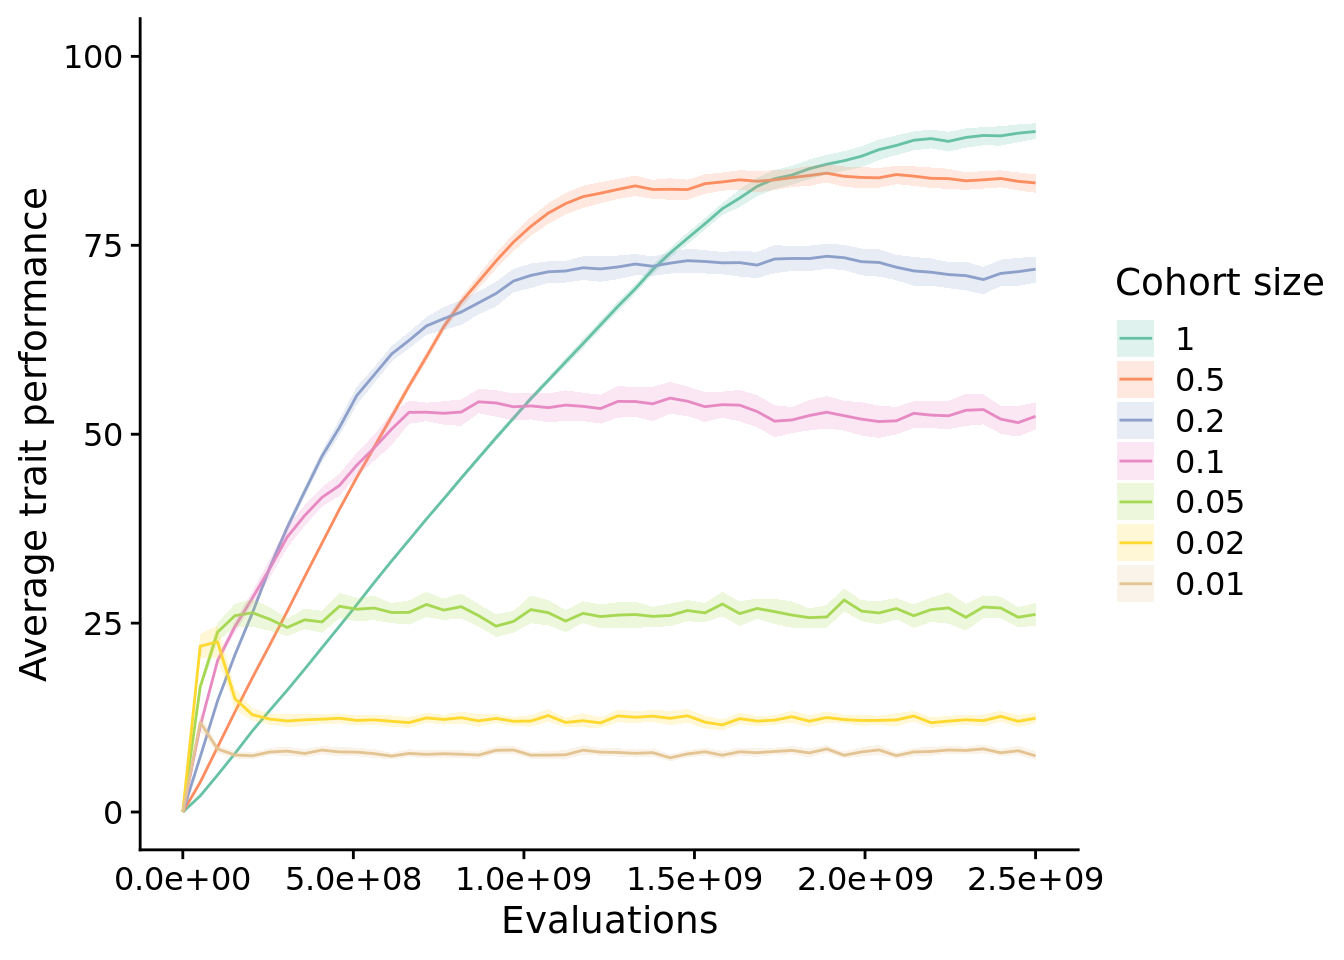
\includegraphics{supplemental-material_files/figure-latex/unnamed-chunk-63-1.pdf}

\hypertarget{final-performance-5}{%
\subsection{Final performance}\label{final-performance-5}}

\begin{Shaded}
\begin{Highlighting}[]
\NormalTok{elite_final_performance_fig <-}\StringTok{ }\KeywordTok{ggplot}\NormalTok{(}
\NormalTok{    final_data,}
    \KeywordTok{aes}\NormalTok{(}\DataTypeTok{x=}\NormalTok{proportion, }\DataTypeTok{y=}\NormalTok{elite_trait_avg, }\DataTypeTok{fill=}\NormalTok{proportion)}
\NormalTok{  ) }\OperatorTok{+}
\StringTok{  }\KeywordTok{geom_flat_violin}\NormalTok{(}
    \DataTypeTok{position =} \KeywordTok{position_nudge}\NormalTok{(}\DataTypeTok{x =} \FloatTok{.2}\NormalTok{, }\DataTypeTok{y =} \DecValTok{0}\NormalTok{),}
    \DataTypeTok{alpha =} \FloatTok{.8}\NormalTok{,}
    \DataTypeTok{scale=}\StringTok{"width"}
\NormalTok{  ) }\OperatorTok{+}
\StringTok{  }\KeywordTok{geom_point}\NormalTok{(}
    \DataTypeTok{mapping=}\KeywordTok{aes}\NormalTok{(}\DataTypeTok{color=}\NormalTok{proportion),}
    \DataTypeTok{position =} \KeywordTok{position_jitter}\NormalTok{(}\DataTypeTok{width =} \FloatTok{.15}\NormalTok{),}
    \DataTypeTok{size =} \FloatTok{.5}\NormalTok{,}
    \DataTypeTok{alpha =} \FloatTok{0.8}
\NormalTok{  ) }\OperatorTok{+}
\StringTok{  }\KeywordTok{geom_boxplot}\NormalTok{(}
    \DataTypeTok{width =} \FloatTok{.1}\NormalTok{,}
    \DataTypeTok{outlier.shape =} \OtherTok{NA}\NormalTok{,}
    \DataTypeTok{alpha =} \FloatTok{0.5}
\NormalTok{  ) }\OperatorTok{+}
\StringTok{  }\KeywordTok{scale_y_continuous}\NormalTok{(}
    \DataTypeTok{name=}\StringTok{"Average trait performance"}\NormalTok{,}
    \DataTypeTok{limits=}\KeywordTok{c}\NormalTok{(}\DecValTok{0}\NormalTok{, }\DecValTok{100}\NormalTok{)}
\NormalTok{  ) }\OperatorTok{+}
\StringTok{  }\KeywordTok{scale_x_discrete}\NormalTok{(}
    \DataTypeTok{name=}\StringTok{"Cohort size"}
\NormalTok{  ) }\OperatorTok{+}
\StringTok{  }\KeywordTok{scale_fill_brewer}\NormalTok{(}
    \DataTypeTok{name=}\StringTok{"Cohort size"}\NormalTok{,}
    \DataTypeTok{palette=}\NormalTok{cb_palette}
\NormalTok{  ) }\OperatorTok{+}
\StringTok{  }\KeywordTok{scale_color_brewer}\NormalTok{(}
    \DataTypeTok{name=}\StringTok{"Cohort size"}\NormalTok{,}
    \DataTypeTok{palette=}\NormalTok{cb_palette}
\NormalTok{  ) }\OperatorTok{+}
\StringTok{  }\KeywordTok{theme}\NormalTok{(}
    \DataTypeTok{legend.position=}\StringTok{"none"}
\NormalTok{  )}
\NormalTok{elite_final_performance_fig}
\end{Highlighting}
\end{Shaded}

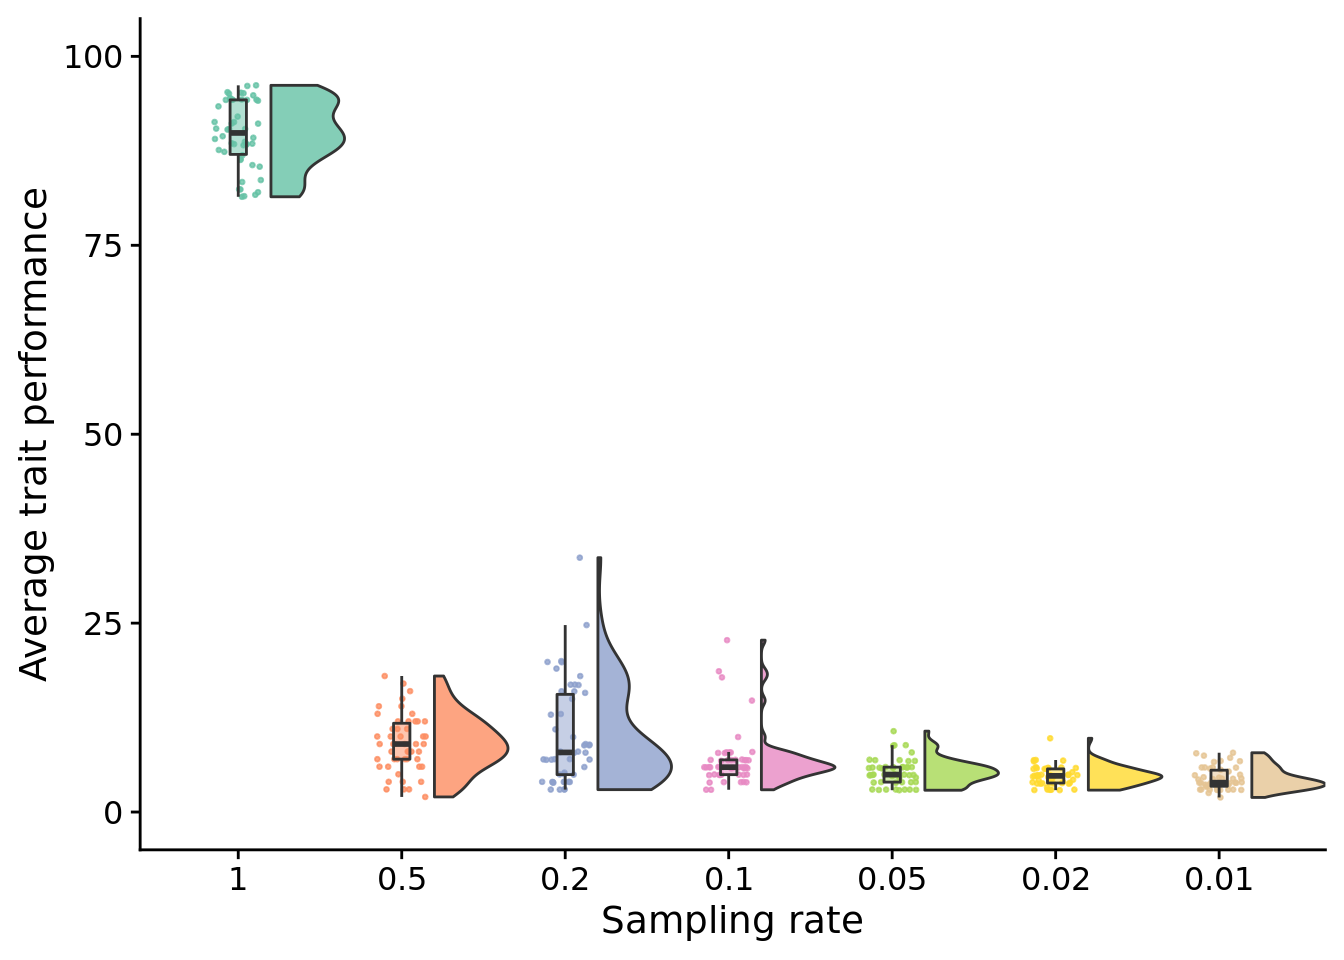
\includegraphics{supplemental-material_files/figure-latex/unnamed-chunk-64-1.pdf}

\hypertarget{unique-starting-positions-5}{%
\section{Unique starting positions}\label{unique-starting-positions-5}}

\begin{Shaded}
\begin{Highlighting}[]
\NormalTok{unique_start_position_coverage_fig <-}\StringTok{ }\KeywordTok{ggplot}\NormalTok{(}
\NormalTok{    data,}
    \KeywordTok{aes}\NormalTok{(}
      \DataTypeTok{x=}\NormalTok{evaluations,}
      \DataTypeTok{y=}\NormalTok{unique_start_positions_coverage,}
      \DataTypeTok{color=}\NormalTok{proportion,}
      \DataTypeTok{fill=}\NormalTok{proportion}
\NormalTok{    )}
\NormalTok{  ) }\OperatorTok{+}
\StringTok{  }\KeywordTok{stat_summary}\NormalTok{(}\DataTypeTok{geom=}\StringTok{"line"}\NormalTok{, }\DataTypeTok{fun=}\NormalTok{mean) }\OperatorTok{+}
\StringTok{  }\KeywordTok{stat_summary}\NormalTok{(}
    \DataTypeTok{geom=}\StringTok{"ribbon"}\NormalTok{,}
    \DataTypeTok{fun.data=}\StringTok{"mean_cl_boot"}\NormalTok{,}
    \DataTypeTok{fun.args=}\KeywordTok{list}\NormalTok{(}\DataTypeTok{conf.int=}\FloatTok{0.95}\NormalTok{),}
    \DataTypeTok{alpha=}\FloatTok{0.2}\NormalTok{,}
    \DataTypeTok{linetype=}\DecValTok{0}
\NormalTok{  ) }\OperatorTok{+}
\StringTok{  }\KeywordTok{scale_y_continuous}\NormalTok{(}
    \DataTypeTok{name=}\StringTok{"Activation position coverage"}\NormalTok{,}
    \DataTypeTok{limits=}\KeywordTok{c}\NormalTok{(}\FloatTok{0.0}\NormalTok{, }\FloatTok{1.0}\NormalTok{)}
\NormalTok{  ) }\OperatorTok{+}
\StringTok{  }\KeywordTok{scale_x_continuous}\NormalTok{(}
    \DataTypeTok{name=}\StringTok{"Evaluations"}
\NormalTok{  ) }\OperatorTok{+}
\StringTok{  }\KeywordTok{scale_fill_brewer}\NormalTok{(}
    \DataTypeTok{name=}\StringTok{"Cohort size"}\NormalTok{,}
    \DataTypeTok{palette=}\NormalTok{cb_palette}
\NormalTok{  ) }\OperatorTok{+}
\StringTok{  }\KeywordTok{scale_color_brewer}\NormalTok{(}
    \DataTypeTok{name=}\StringTok{"Cohort size"}\NormalTok{,}
    \DataTypeTok{palette=}\NormalTok{cb_palette}
\NormalTok{  )}
\NormalTok{unique_start_position_coverage_fig}
\end{Highlighting}
\end{Shaded}

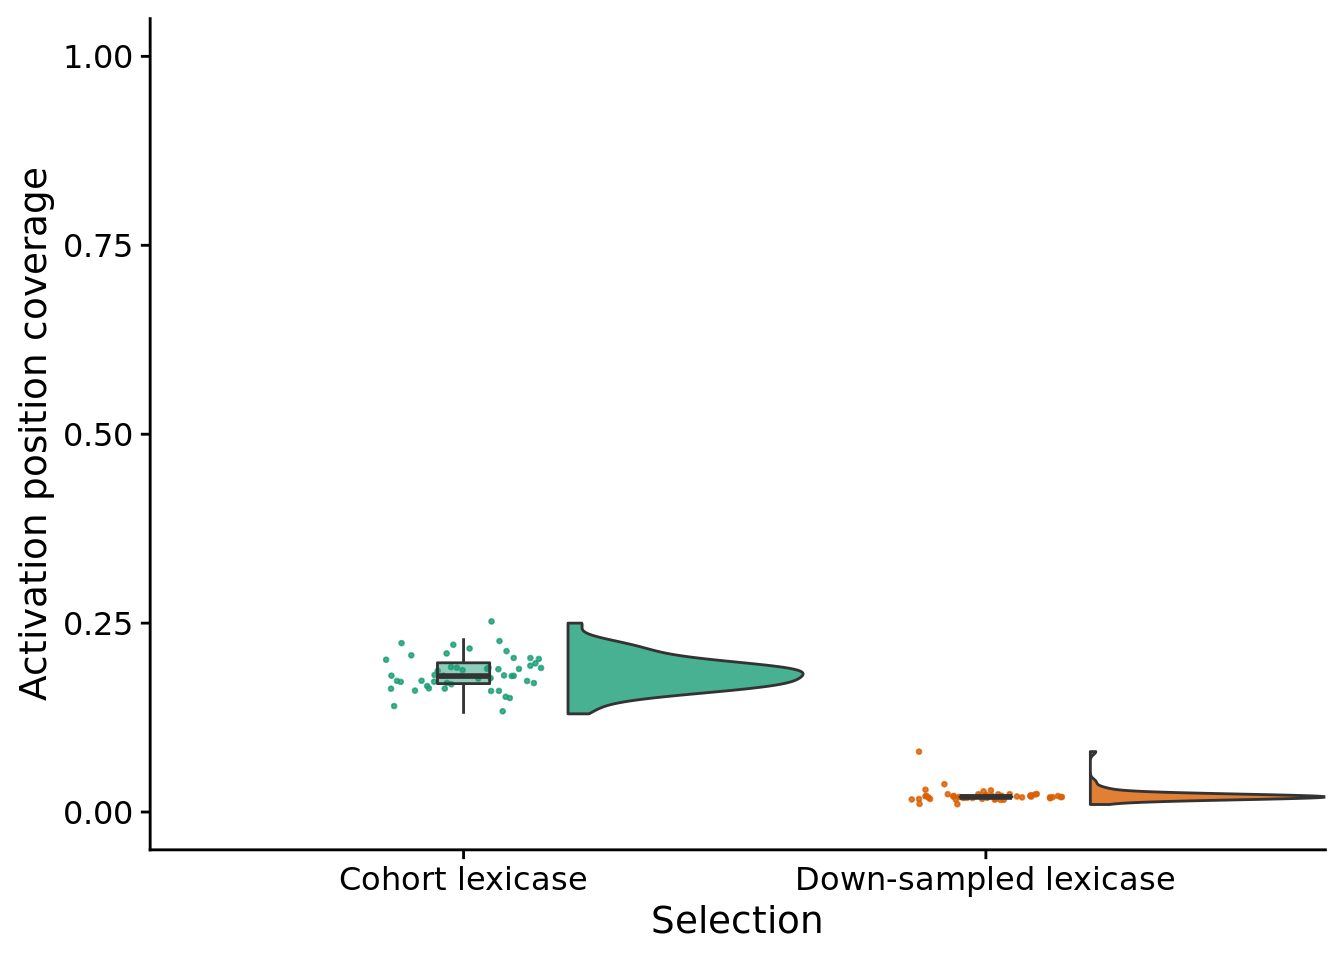
\includegraphics{supplemental-material_files/figure-latex/unnamed-chunk-65-1.pdf}

\hypertarget{final-starting-position-coverage-4}{%
\subsection{Final starting position coverage}\label{final-starting-position-coverage-4}}

\begin{Shaded}
\begin{Highlighting}[]
\NormalTok{unique_start_positions_coverage_final_fig <-}\StringTok{ }\KeywordTok{ggplot}\NormalTok{(}
\NormalTok{    final_data,}
    \KeywordTok{aes}\NormalTok{(}
      \DataTypeTok{x=}\NormalTok{proportion,}
      \DataTypeTok{y=}\NormalTok{unique_start_positions_coverage,}
      \DataTypeTok{fill=}\NormalTok{proportion}
\NormalTok{    )}
\NormalTok{  ) }\OperatorTok{+}
\StringTok{  }\KeywordTok{geom_flat_violin}\NormalTok{(}
    \DataTypeTok{position =} \KeywordTok{position_nudge}\NormalTok{(}\DataTypeTok{x =} \FloatTok{.2}\NormalTok{, }\DataTypeTok{y =} \DecValTok{0}\NormalTok{),}
    \DataTypeTok{alpha =} \FloatTok{.8}\NormalTok{,}
    \DataTypeTok{scale=}\StringTok{"width"}
\NormalTok{  ) }\OperatorTok{+}
\StringTok{  }\KeywordTok{geom_point}\NormalTok{(}
    \DataTypeTok{mapping=}\KeywordTok{aes}\NormalTok{(}\DataTypeTok{color=}\NormalTok{proportion),}
    \DataTypeTok{position =} \KeywordTok{position_jitter}\NormalTok{(}\DataTypeTok{width =} \FloatTok{.15}\NormalTok{),}
    \DataTypeTok{size =} \FloatTok{.5}\NormalTok{,}
    \DataTypeTok{alpha =} \FloatTok{0.8}
\NormalTok{  ) }\OperatorTok{+}
\StringTok{  }\KeywordTok{geom_boxplot}\NormalTok{(}
    \DataTypeTok{width =} \FloatTok{.1}\NormalTok{,}
    \DataTypeTok{outlier.shape =} \OtherTok{NA}\NormalTok{,}
    \DataTypeTok{alpha =} \FloatTok{0.5}
\NormalTok{  ) }\OperatorTok{+}
\StringTok{  }\KeywordTok{scale_y_continuous}\NormalTok{(}
    \DataTypeTok{name=}\StringTok{"Activation position coverage"}\NormalTok{,}
    \DataTypeTok{limits=}\KeywordTok{c}\NormalTok{(}\DecValTok{0}\NormalTok{, }\FloatTok{1.0}\NormalTok{)}
\NormalTok{  ) }\OperatorTok{+}
\StringTok{  }\KeywordTok{scale_x_discrete}\NormalTok{(}
    \DataTypeTok{name=}\StringTok{"Cohort size"}
\NormalTok{  ) }\OperatorTok{+}
\StringTok{  }\KeywordTok{scale_fill_brewer}\NormalTok{(}
    \DataTypeTok{name=}\StringTok{"Cohort size"}\NormalTok{,}
    \DataTypeTok{palette=}\NormalTok{cb_palette}
\NormalTok{  ) }\OperatorTok{+}
\StringTok{  }\KeywordTok{scale_color_brewer}\NormalTok{(}
    \DataTypeTok{name=}\StringTok{"Cohort size"}\NormalTok{,}
    \DataTypeTok{palette=}\NormalTok{cb_palette}
\NormalTok{  ) }\OperatorTok{+}
\StringTok{  }\KeywordTok{theme}\NormalTok{(}
    \DataTypeTok{legend.position=}\StringTok{"none"}
\NormalTok{  )}
\NormalTok{unique_start_positions_coverage_final_fig}
\end{Highlighting}
\end{Shaded}

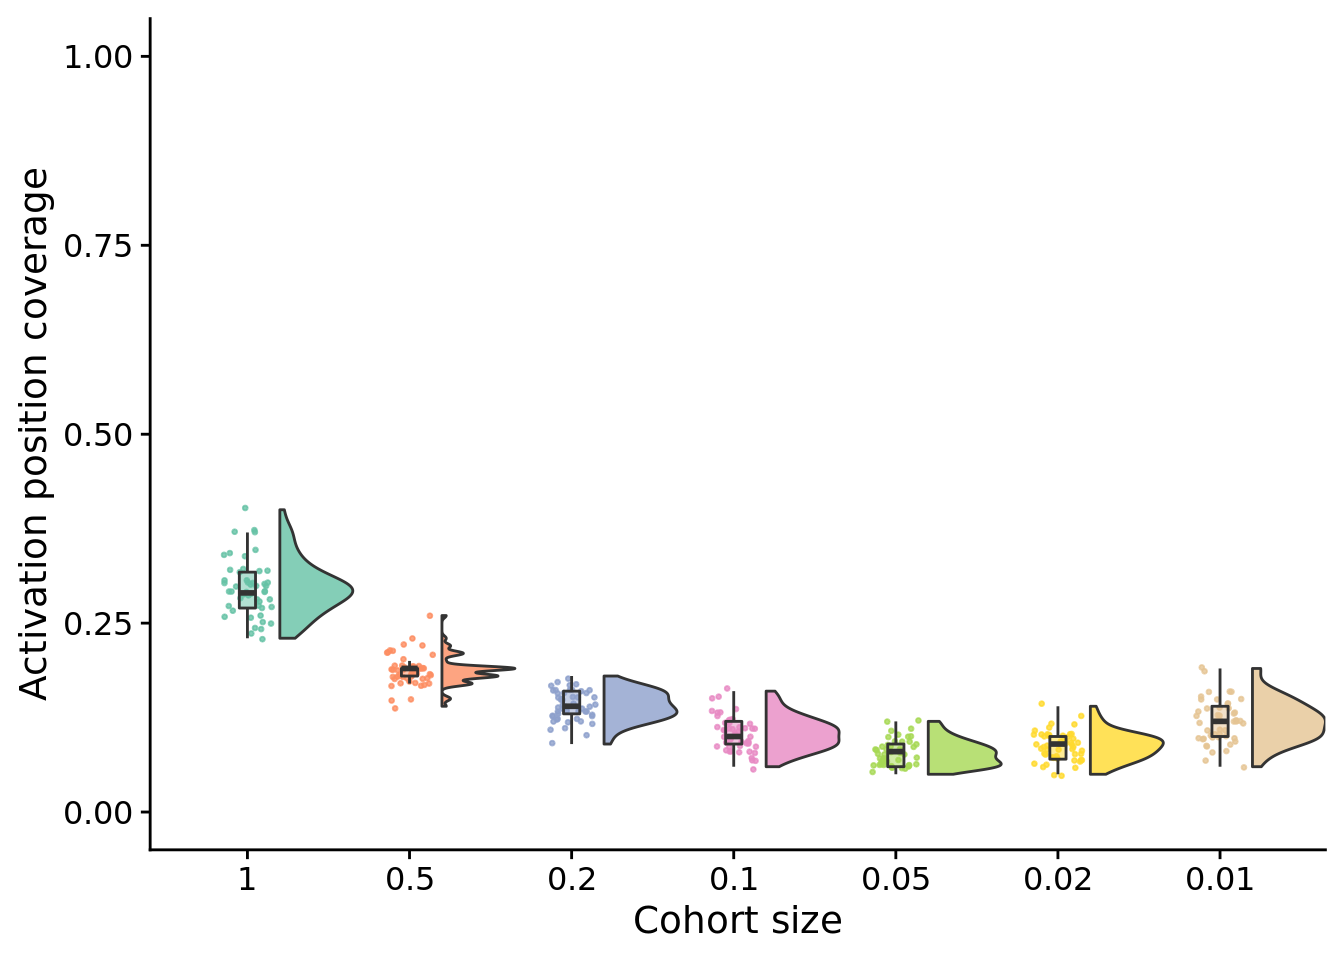
\includegraphics{supplemental-material_files/figure-latex/unnamed-chunk-66-1.pdf}

\hypertarget{manuscript-figures-5}{%
\section{Manuscript figures}\label{manuscript-figures-5}}

\begin{Shaded}
\begin{Highlighting}[]
\NormalTok{legend <-}\StringTok{ }\NormalTok{cowplot}\OperatorTok{::}\KeywordTok{get_legend}\NormalTok{(}
\NormalTok{    elite_ave_performance_fig }\OperatorTok{+}
\StringTok{      }\KeywordTok{guides}\NormalTok{(}
        \DataTypeTok{color=}\KeywordTok{guide_legend}\NormalTok{(}\DataTypeTok{nrow=}\DecValTok{1}\NormalTok{),}
        \DataTypeTok{fill=}\KeywordTok{guide_legend}\NormalTok{(}\DataTypeTok{nrow=}\DecValTok{1}\NormalTok{)}
\NormalTok{      ) }\OperatorTok{+}
\StringTok{      }\KeywordTok{theme}\NormalTok{(}
        \DataTypeTok{legend.position =} \StringTok{"bottom"}\NormalTok{,}
        \DataTypeTok{legend.box=}\StringTok{"horizontal"}\NormalTok{,}
        \DataTypeTok{legend.justification=}\StringTok{"center"}
\NormalTok{      )}
\NormalTok{  )}

\NormalTok{grid <-}\StringTok{ }\KeywordTok{plot_grid}\NormalTok{(}
\NormalTok{  elite_ave_performance_fig }\OperatorTok{+}
\StringTok{    }\KeywordTok{ggtitle}\NormalTok{(}\StringTok{"Performance over time"}\NormalTok{) }\OperatorTok{+}
\StringTok{    }\KeywordTok{theme}\NormalTok{(}\DataTypeTok{legend.position=}\StringTok{"none"}\NormalTok{),}
\NormalTok{  elite_final_performance_fig }\OperatorTok{+}
\StringTok{    }\KeywordTok{ggtitle}\NormalTok{(}\StringTok{"Final performance"}\NormalTok{) }\OperatorTok{+}
\StringTok{    }\KeywordTok{theme}\NormalTok{(),}
\NormalTok{  unique_start_position_coverage_fig }\OperatorTok{+}
\StringTok{    }\KeywordTok{ggtitle}\NormalTok{(}\StringTok{"Activation position coverage over time"}\NormalTok{) }\OperatorTok{+}
\StringTok{    }\KeywordTok{theme}\NormalTok{(}\DataTypeTok{legend.position=}\StringTok{"none"}\NormalTok{),}
\NormalTok{  unique_start_positions_coverage_final_fig }\OperatorTok{+}
\StringTok{    }\KeywordTok{ggtitle}\NormalTok{(}\StringTok{"Final activation position coverage"}\NormalTok{) }\OperatorTok{+}
\StringTok{    }\KeywordTok{theme}\NormalTok{(),}
  \DataTypeTok{nrow=}\DecValTok{2}\NormalTok{,}
  \DataTypeTok{ncol=}\DecValTok{2}\NormalTok{,}
  \DataTypeTok{rel_widths=}\KeywordTok{c}\NormalTok{(}\DecValTok{3}\NormalTok{,}\DecValTok{2}\NormalTok{),}
  \DataTypeTok{labels=}\StringTok{"auto"}
\NormalTok{)}

\NormalTok{grid <-}\StringTok{ }\KeywordTok{plot_grid}\NormalTok{(}
\NormalTok{  grid,}
\NormalTok{  legend,}
  \DataTypeTok{nrow=}\DecValTok{2}\NormalTok{,}
  \DataTypeTok{ncol=}\DecValTok{1}\NormalTok{,}
  \DataTypeTok{rel_heights=}\KeywordTok{c}\NormalTok{(}\DecValTok{1}\NormalTok{, }\FloatTok{0.1}\NormalTok{)}
\NormalTok{)}

\KeywordTok{save_plot}\NormalTok{(}
  \KeywordTok{paste}\NormalTok{(working_directory, }\StringTok{"imgs/cohort-panel.pdf"}\NormalTok{, }\DataTypeTok{sep=}\StringTok{""}\NormalTok{),}
\NormalTok{  grid,}
  \DataTypeTok{base_width=}\DecValTok{12}\NormalTok{,}
  \DataTypeTok{base_height=}\DecValTok{8}
\NormalTok{)}

\NormalTok{grid}
\end{Highlighting}
\end{Shaded}

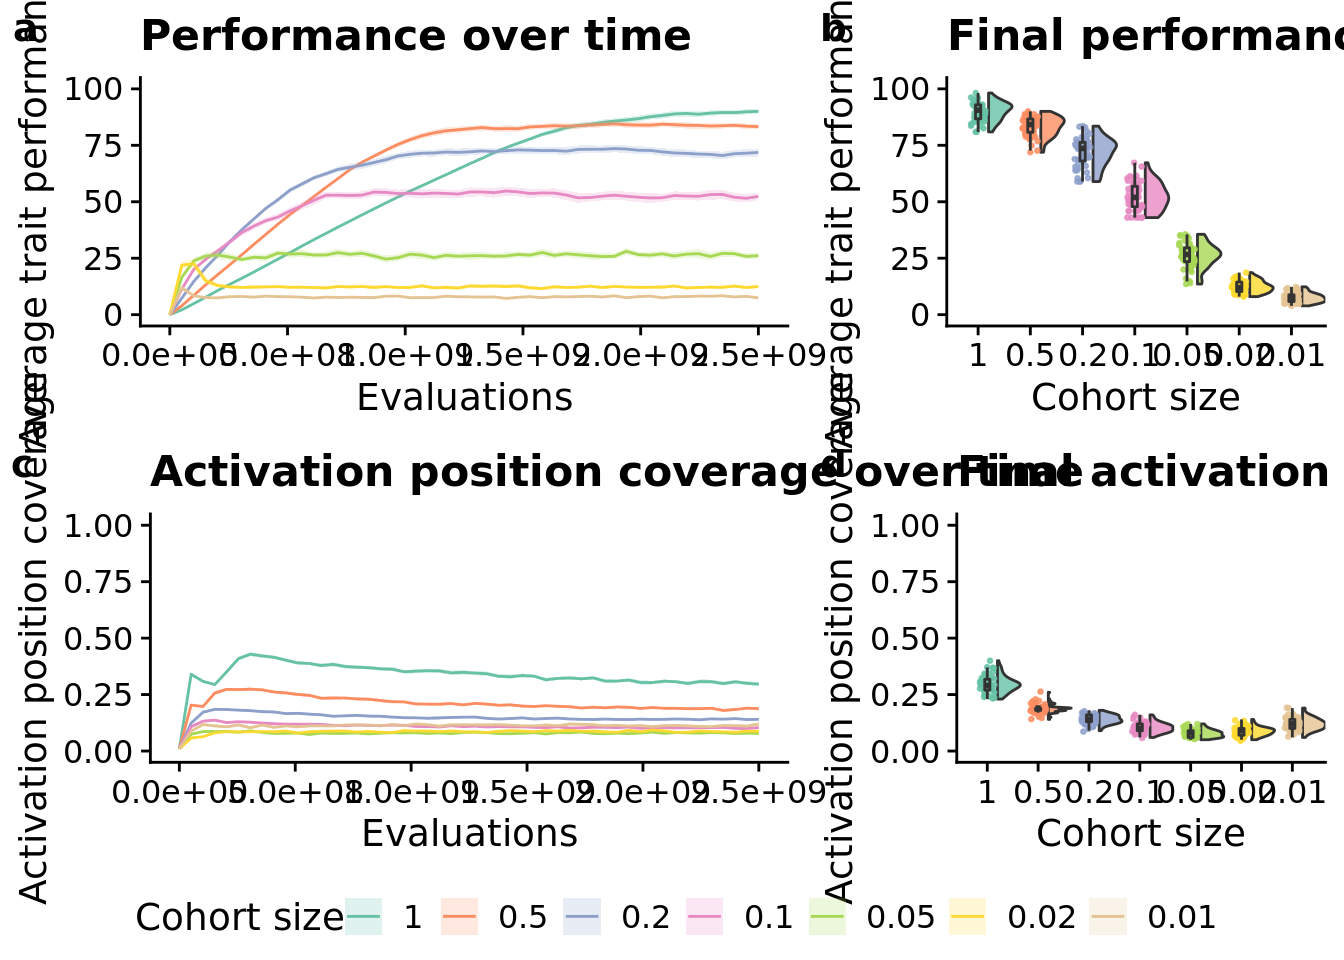
\includegraphics{supplemental-material_files/figure-latex/unnamed-chunk-67-1.pdf}

\hypertarget{down-sampled-lexicase-versus-cohort-lexicase}{%
\chapter{Down-sampled lexicase versus cohort lexicase}\label{down-sampled-lexicase-versus-cohort-lexicase}}

\hypertarget{overview-6}{%
\section{Overview}\label{overview-6}}

\begin{Shaded}
\begin{Highlighting}[]
\CommentTok{# Relative location of data.}
\NormalTok{working_directory <-}
\StringTok{  "experiments/2021-06-05-downsample-vs-cohort/analysis/"}
\CommentTok{# working_directory <- "./"}

\CommentTok{# Settings for visualization}
\NormalTok{cb_palette <-}\StringTok{ "Dark2"}
\CommentTok{# Create directory to dump plots}
\KeywordTok{dir.create}\NormalTok{(}\KeywordTok{paste0}\NormalTok{(working_directory, }\StringTok{"imgs"}\NormalTok{), }\DataTypeTok{showWarnings=}\OtherTok{FALSE}\NormalTok{)}
\end{Highlighting}
\end{Shaded}

\hypertarget{analysis-dependencies-6}{%
\section{Analysis dependencies}\label{analysis-dependencies-6}}

\begin{Shaded}
\begin{Highlighting}[]
\KeywordTok{library}\NormalTok{(ggplot2)}
\KeywordTok{library}\NormalTok{(tidyverse)}
\KeywordTok{library}\NormalTok{(knitr)}
\KeywordTok{library}\NormalTok{(cowplot)}
\KeywordTok{library}\NormalTok{(viridis)}
\KeywordTok{library}\NormalTok{(RColorBrewer)}
\KeywordTok{library}\NormalTok{(rstatix)}
\KeywordTok{library}\NormalTok{(ggsignif)}
\KeywordTok{library}\NormalTok{(Hmisc)}
\KeywordTok{source}\NormalTok{(}\StringTok{"https://gist.githubusercontent.com/benmarwick/2a1bb0133ff568cbe28d/raw/fb53bd97121f7f9ce947837ef1a4c65a73bffb3f/geom_flat_violin.R"}\NormalTok{)}
\end{Highlighting}
\end{Shaded}

These analyses were conducted in the following computing environment:

\begin{Shaded}
\begin{Highlighting}[]
\KeywordTok{print}\NormalTok{(version)}
\end{Highlighting}
\end{Shaded}

\begin{verbatim}
##                _                           
## platform       x86_64-pc-linux-gnu         
## arch           x86_64                      
## os             linux-gnu                   
## system         x86_64, linux-gnu           
## status                                     
## major          4                           
## minor          1.0                         
## year           2021                        
## month          05                          
## day            18                          
## svn rev        80317                       
## language       R                           
## version.string R version 4.1.0 (2021-05-18)
## nickname       Camp Pontanezen
\end{verbatim}

\hypertarget{setup-6}{%
\section{Setup}\label{setup-6}}

\begin{Shaded}
\begin{Highlighting}[]
\NormalTok{data_loc <-}\StringTok{ }\KeywordTok{paste0}\NormalTok{(working_directory, }\StringTok{"data/timeseries.csv"}\NormalTok{)}
\NormalTok{data <-}\StringTok{ }\KeywordTok{read.csv}\NormalTok{(data_loc, }\DataTypeTok{na.strings=}\StringTok{"NONE"}\NormalTok{)}

\NormalTok{data}\OperatorTok{$}\NormalTok{cardinality <-}\StringTok{ }\KeywordTok{as.factor}\NormalTok{(}
\NormalTok{  data}\OperatorTok{$}\NormalTok{OBJECTIVE_CNT}
\NormalTok{)}
\NormalTok{data}\OperatorTok{$}\NormalTok{selection_name <-}\StringTok{ }\KeywordTok{as.factor}\NormalTok{(}
\NormalTok{  data}\OperatorTok{$}\NormalTok{selection_name}
\NormalTok{)}

\NormalTok{data}\OperatorTok{$}\NormalTok{epsilon <-}\StringTok{ }\KeywordTok{as.factor}\NormalTok{(}
\NormalTok{  data}\OperatorTok{$}\NormalTok{LEX_EPS}
\NormalTok{)}

\CommentTok{# I always set cohort and downsampled lexicase sampling rates to}
\CommentTok{# be the same on a given run (regardless of selection scheme)}
\NormalTok{data}\OperatorTok{$}\NormalTok{proportion <-}\StringTok{ }\KeywordTok{factor}\NormalTok{(}
\NormalTok{  data}\OperatorTok{$}\NormalTok{COH_LEX_PROP,}
  \DataTypeTok{levels=}\KeywordTok{c}\NormalTok{(}\DecValTok{1}\NormalTok{, }\FloatTok{0.5}\NormalTok{, }\FloatTok{0.2}\NormalTok{, }\FloatTok{0.1}\NormalTok{, }\FloatTok{0.05}\NormalTok{, }\FloatTok{0.02}\NormalTok{, }\FloatTok{0.01}\NormalTok{)}
\NormalTok{)}

\NormalTok{data}\OperatorTok{$}\NormalTok{elite_trait_avg <-}
\StringTok{  }\NormalTok{data}\OperatorTok{$}\NormalTok{ele_agg_per }\OperatorTok{/}\StringTok{ }\NormalTok{data}\OperatorTok{$}\NormalTok{OBJECTIVE_CNT}
\NormalTok{data}\OperatorTok{$}\NormalTok{unique_start_positions_coverage <-}
\StringTok{  }\NormalTok{data}\OperatorTok{$}\NormalTok{uni_str_pos }\OperatorTok{/}\StringTok{ }\NormalTok{data}\OperatorTok{$}\NormalTok{OBJECTIVE_CNT}

\NormalTok{final_data <-}\StringTok{ }\KeywordTok{filter}\NormalTok{(data, evaluations}\OperatorTok{==}\KeywordTok{max}\NormalTok{(data}\OperatorTok{$}\NormalTok{evaluations))}

\CommentTok{# Labeler for stats annotations}
\NormalTok{p_label <-}\StringTok{ }\ControlFlowTok{function}\NormalTok{(p_value) \{}
\NormalTok{  threshold =}\StringTok{ }\FloatTok{0.0001}
  \ControlFlowTok{if}\NormalTok{ (p_value }\OperatorTok{<}\StringTok{ }\NormalTok{threshold) \{}
    \KeywordTok{return}\NormalTok{(}\KeywordTok{paste0}\NormalTok{(}\StringTok{"p < "}\NormalTok{, threshold))}
\NormalTok{  \} }\ControlFlowTok{else}\NormalTok{ \{}
    \KeywordTok{return}\NormalTok{(}\KeywordTok{paste0}\NormalTok{(}\StringTok{"p = "}\NormalTok{, p_value))}
\NormalTok{  \}}
\NormalTok{\}}

\CommentTok{# Significance threshold}
\NormalTok{alpha <-}\StringTok{ }\FloatTok{0.05}

\CommentTok{####### misc #######}
\CommentTok{# Configure our default graphing theme}
\KeywordTok{theme_set}\NormalTok{(}\KeywordTok{theme_cowplot}\NormalTok{())}
\end{Highlighting}
\end{Shaded}

\hypertarget{exploration-diagnostic-performance-6}{%
\section{Exploration diagnostic performance}\label{exploration-diagnostic-performance-6}}

\begin{Shaded}
\begin{Highlighting}[]
\NormalTok{elite_ave_performance_fig <-}
\StringTok{  }\KeywordTok{ggplot}\NormalTok{(}
\NormalTok{    data,}
    \KeywordTok{aes}\NormalTok{(}
      \DataTypeTok{x=}\NormalTok{gen,}
      \DataTypeTok{y=}\NormalTok{elite_trait_avg,}
      \DataTypeTok{color=}\NormalTok{selection_name,}
      \DataTypeTok{fill=}\NormalTok{selection_name}
\NormalTok{    )}
\NormalTok{  ) }\OperatorTok{+}
\StringTok{  }\KeywordTok{stat_summary}\NormalTok{(}\DataTypeTok{geom=}\StringTok{"line"}\NormalTok{, }\DataTypeTok{fun=}\NormalTok{mean) }\OperatorTok{+}
\StringTok{  }\KeywordTok{stat_summary}\NormalTok{(}
    \DataTypeTok{geom=}\StringTok{"ribbon"}\NormalTok{,}
    \DataTypeTok{fun.data=}\StringTok{"mean_cl_boot"}\NormalTok{,}
    \DataTypeTok{fun.args=}\KeywordTok{list}\NormalTok{(}\DataTypeTok{conf.int=}\FloatTok{0.95}\NormalTok{),}
    \DataTypeTok{alpha=}\FloatTok{0.2}\NormalTok{,}
    \DataTypeTok{linetype=}\DecValTok{0}
\NormalTok{  ) }\OperatorTok{+}
\StringTok{  }\KeywordTok{scale_y_continuous}\NormalTok{(}
    \DataTypeTok{name=}\StringTok{"Average trait performance"}\NormalTok{,}
    \DataTypeTok{limits=}\KeywordTok{c}\NormalTok{(}\DecValTok{0}\NormalTok{, }\DecValTok{100}\NormalTok{)}
\NormalTok{  ) }\OperatorTok{+}
\StringTok{  }\KeywordTok{scale_x_continuous}\NormalTok{(}
    \DataTypeTok{name=}\StringTok{"Generations"}
\NormalTok{  ) }\OperatorTok{+}
\StringTok{  }\KeywordTok{scale_fill_brewer}\NormalTok{(}
    \DataTypeTok{name=}\StringTok{"Selection"}\NormalTok{,}
    \DataTypeTok{palette=}\NormalTok{cb_palette,}
    \DataTypeTok{limits=}\KeywordTok{c}\NormalTok{(}\StringTok{"CohortLexicase"}\NormalTok{, }\StringTok{"DownSampledLexicase"}\NormalTok{),}
    \DataTypeTok{labels=}\KeywordTok{c}\NormalTok{(}\StringTok{"Cohort lexicase"}\NormalTok{, }\StringTok{"Down-sampled lexicase"}\NormalTok{)}
\NormalTok{  ) }\OperatorTok{+}
\StringTok{  }\KeywordTok{scale_color_brewer}\NormalTok{(}
    \DataTypeTok{name=}\StringTok{"Selection"}\NormalTok{,}
    \DataTypeTok{palette=}\NormalTok{cb_palette,}
    \DataTypeTok{limits=}\KeywordTok{c}\NormalTok{(}\StringTok{"CohortLexicase"}\NormalTok{, }\StringTok{"DownSampledLexicase"}\NormalTok{),}
    \DataTypeTok{labels=}\KeywordTok{c}\NormalTok{(}\StringTok{"Cohort lexicase"}\NormalTok{, }\StringTok{"Down-sampled lexicase"}\NormalTok{)}
\NormalTok{  )}
\NormalTok{elite_ave_performance_fig}
\end{Highlighting}
\end{Shaded}

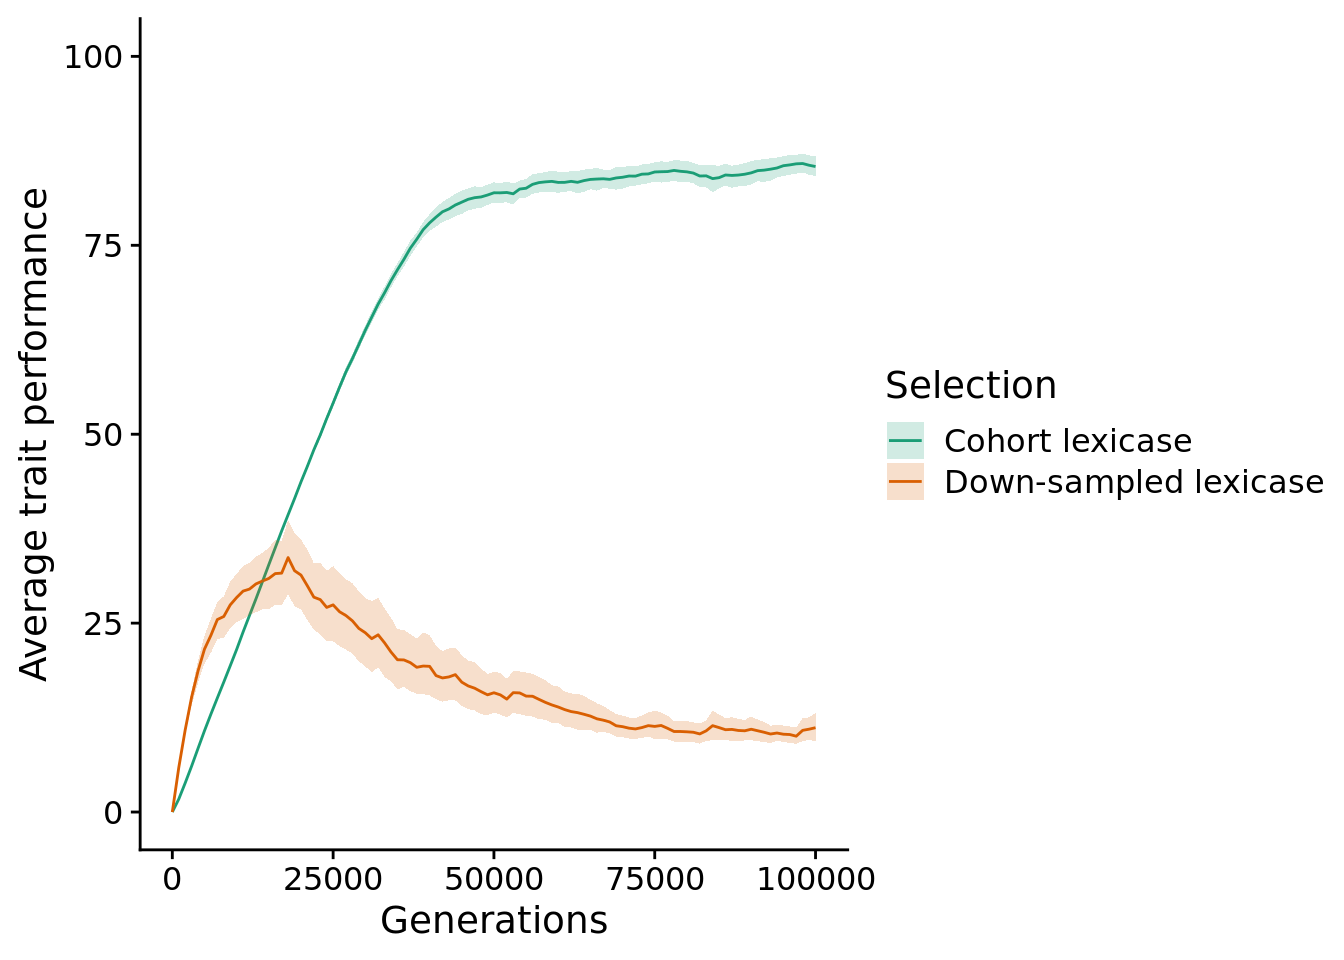
\includegraphics{supplemental-material_files/figure-latex/unnamed-chunk-72-1.pdf}

\hypertarget{final-performance-6}{%
\subsection{Final performance}\label{final-performance-6}}

\begin{Shaded}
\begin{Highlighting}[]
\CommentTok{# Compute manual labels for geom_signif}
\NormalTok{stat.test <-}\StringTok{ }\NormalTok{final_data }\OperatorTok
\StringTok{  }\KeywordTok{wilcox_test}\NormalTok{(elite_trait_avg }\OperatorTok{~}\StringTok{ }\NormalTok{selection_name) }\OperatorTok
\StringTok{  }\KeywordTok{adjust_pvalue}\NormalTok{(}\DataTypeTok{method =} \StringTok{"bonferroni"}\NormalTok{) }\OperatorTok
\StringTok{  }\KeywordTok{add_significance}\NormalTok{() }\OperatorTok
\StringTok{  }\KeywordTok{add_xy_position}\NormalTok{(}\DataTypeTok{x=}\StringTok{"selection_name"}\NormalTok{,}\DataTypeTok{step.increase=}\DecValTok{1}\NormalTok{)}
\NormalTok{stat.test}\OperatorTok{$}\NormalTok{manual_position <-}\StringTok{ }\NormalTok{stat.test}\OperatorTok{$}\NormalTok{y.position }\OperatorTok{*}\StringTok{ }\FloatTok{1.05}
\NormalTok{stat.test}\OperatorTok{$}\NormalTok{label <-}\StringTok{ }\KeywordTok{mapply}\NormalTok{(p_label,stat.test}\OperatorTok{$}\NormalTok{p.adj)}
\end{Highlighting}
\end{Shaded}

\begin{Shaded}
\begin{Highlighting}[]
\NormalTok{elite_final_performance_fig <-}\StringTok{ }\KeywordTok{ggplot}\NormalTok{(}
\NormalTok{    final_data,}
    \KeywordTok{aes}\NormalTok{(}\DataTypeTok{x=}\NormalTok{selection_name, }\DataTypeTok{y=}\NormalTok{elite_trait_avg, }\DataTypeTok{fill=}\NormalTok{selection_name)}
\NormalTok{  ) }\OperatorTok{+}
\StringTok{  }\KeywordTok{geom_flat_violin}\NormalTok{(}
    \DataTypeTok{position =} \KeywordTok{position_nudge}\NormalTok{(}\DataTypeTok{x =} \FloatTok{.2}\NormalTok{, }\DataTypeTok{y =} \DecValTok{0}\NormalTok{),}
    \DataTypeTok{alpha =} \FloatTok{.8}\NormalTok{,}
    \DataTypeTok{scale=}\StringTok{"width"}
\NormalTok{  ) }\OperatorTok{+}
\StringTok{  }\KeywordTok{geom_point}\NormalTok{(}
    \DataTypeTok{mapping=}\KeywordTok{aes}\NormalTok{(}\DataTypeTok{color=}\NormalTok{selection_name),}
    \DataTypeTok{position =} \KeywordTok{position_jitter}\NormalTok{(}\DataTypeTok{width =} \FloatTok{.15}\NormalTok{),}
    \DataTypeTok{size =} \FloatTok{.5}\NormalTok{,}
    \DataTypeTok{alpha =} \FloatTok{0.8}
\NormalTok{  ) }\OperatorTok{+}
\StringTok{  }\KeywordTok{geom_boxplot}\NormalTok{(}
    \DataTypeTok{width =} \FloatTok{.1}\NormalTok{,}
    \DataTypeTok{outlier.shape =} \OtherTok{NA}\NormalTok{,}
    \DataTypeTok{alpha =} \FloatTok{0.5}
\NormalTok{  ) }\OperatorTok{+}
\StringTok{  }\KeywordTok{scale_y_continuous}\NormalTok{(}
    \DataTypeTok{name=}\StringTok{"Average trait performance"}\NormalTok{,}
    \DataTypeTok{limits=}\KeywordTok{c}\NormalTok{(}\DecValTok{0}\NormalTok{, }\DecValTok{100}\NormalTok{)}
\NormalTok{  ) }\OperatorTok{+}
\StringTok{  }\KeywordTok{scale_x_discrete}\NormalTok{(}
    \DataTypeTok{name=}\StringTok{"Selection"}\NormalTok{,}
    \DataTypeTok{limits=}\KeywordTok{c}\NormalTok{(}\StringTok{"CohortLexicase"}\NormalTok{, }\StringTok{"DownSampledLexicase"}\NormalTok{),}
    \DataTypeTok{labels=}\KeywordTok{c}\NormalTok{(}\StringTok{"Cohort lexicase"}\NormalTok{, }\StringTok{"Down-sampled lexicase"}\NormalTok{)}
\NormalTok{  ) }\OperatorTok{+}
\StringTok{  }\KeywordTok{scale_fill_brewer}\NormalTok{(}
    \DataTypeTok{name=}\StringTok{"Selection"}\NormalTok{,}
    \DataTypeTok{palette=}\NormalTok{cb_palette,}
    \DataTypeTok{limits=}\KeywordTok{c}\NormalTok{(}\StringTok{"CohortLexicase"}\NormalTok{, }\StringTok{"DownSampledLexicase"}\NormalTok{),}
    \DataTypeTok{labels=}\KeywordTok{c}\NormalTok{(}\StringTok{"Cohort lexicase"}\NormalTok{, }\StringTok{"Down-sampled lexicase"}\NormalTok{)}
\NormalTok{  ) }\OperatorTok{+}
\StringTok{  }\KeywordTok{scale_color_brewer}\NormalTok{(}
    \DataTypeTok{name=}\StringTok{"Selection"}\NormalTok{,}
    \DataTypeTok{palette=}\NormalTok{cb_palette,}
    \DataTypeTok{limits=}\KeywordTok{c}\NormalTok{(}\StringTok{"CohortLexicase"}\NormalTok{, }\StringTok{"DownSampledLexicase"}\NormalTok{),}
    \DataTypeTok{labels=}\KeywordTok{c}\NormalTok{(}\StringTok{"Cohort lexicase"}\NormalTok{, }\StringTok{"Down-sampled lexicase"}\NormalTok{)}
\NormalTok{  ) }\OperatorTok{+}
\StringTok{  }\KeywordTok{theme}\NormalTok{(}
    \DataTypeTok{legend.position=}\StringTok{"none"}
\NormalTok{  )}
\NormalTok{elite_final_performance_fig}
\end{Highlighting}
\end{Shaded}

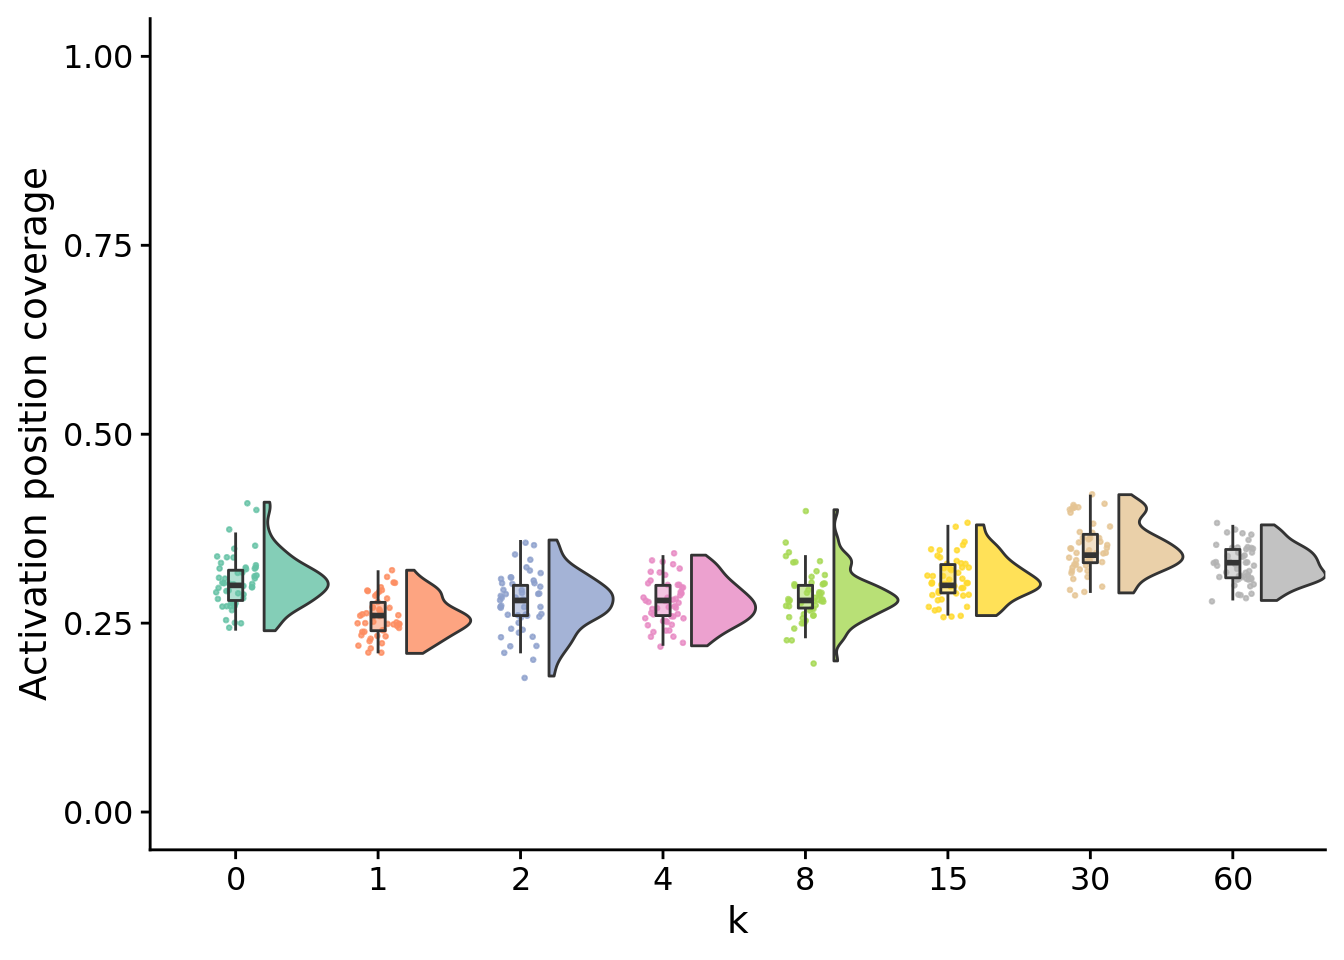
\includegraphics{supplemental-material_files/figure-latex/unnamed-chunk-74-1.pdf}

\begin{tabular}{l|l|l|r|r|r|r|r|l|r|l|r|r|r|l}
\hline
.y. & group1 & group2 & n1 & n2 & statistic & p & p.adj & p.adj.signif & y.position & groups & xmin & xmax & manual\_position & label\\
\hline
elite\_trait\_avg & CohortLexicase & DownSampledLexicase & 50 & 50 & 2500 & 0 & 0 & **** & 150.227 & CohortLexicase     , DownSampledLexicase & 1 & 2 & 157.7383 & p < 1e-04\\
\hline
\end{tabular}

\hypertarget{unique-starting-positions-6}{%
\section{Unique starting positions}\label{unique-starting-positions-6}}

\begin{Shaded}
\begin{Highlighting}[]
\NormalTok{unique_start_position_coverage_fig <-}\StringTok{ }\KeywordTok{ggplot}\NormalTok{(}
\NormalTok{    data,}
    \KeywordTok{aes}\NormalTok{(}
      \DataTypeTok{x=}\NormalTok{gen,}
      \DataTypeTok{y=}\NormalTok{unique_start_positions_coverage,}
      \DataTypeTok{color=}\NormalTok{selection_name,}
      \DataTypeTok{fill=}\NormalTok{selection_name}
\NormalTok{    )}
\NormalTok{  ) }\OperatorTok{+}
\StringTok{  }\KeywordTok{stat_summary}\NormalTok{(}\DataTypeTok{geom=}\StringTok{"line"}\NormalTok{, }\DataTypeTok{fun=}\NormalTok{mean) }\OperatorTok{+}
\StringTok{  }\KeywordTok{stat_summary}\NormalTok{(}
    \DataTypeTok{geom=}\StringTok{"ribbon"}\NormalTok{,}
    \DataTypeTok{fun.data=}\StringTok{"mean_cl_boot"}\NormalTok{,}
    \DataTypeTok{fun.args=}\KeywordTok{list}\NormalTok{(}\DataTypeTok{conf.int=}\FloatTok{0.95}\NormalTok{),}
    \DataTypeTok{alpha=}\FloatTok{0.2}\NormalTok{,}
    \DataTypeTok{linetype=}\DecValTok{0}
\NormalTok{  ) }\OperatorTok{+}
\StringTok{  }\KeywordTok{scale_y_continuous}\NormalTok{(}
    \DataTypeTok{name=}\StringTok{"Activation position coverage"}\NormalTok{,}
    \DataTypeTok{limits=}\KeywordTok{c}\NormalTok{(}\FloatTok{0.0}\NormalTok{, }\FloatTok{1.0}\NormalTok{)}
\NormalTok{  ) }\OperatorTok{+}
\StringTok{  }\KeywordTok{scale_x_continuous}\NormalTok{(}
    \DataTypeTok{name=}\StringTok{"Generations"}
\NormalTok{  ) }\OperatorTok{+}
\StringTok{  }\KeywordTok{scale_fill_brewer}\NormalTok{(}
    \DataTypeTok{name=}\StringTok{"Selection"}\NormalTok{,}
    \DataTypeTok{palette=}\NormalTok{cb_palette,}
    \DataTypeTok{limits=}\KeywordTok{c}\NormalTok{(}\StringTok{"CohortLexicase"}\NormalTok{, }\StringTok{"DownSampledLexicase"}\NormalTok{),}
    \DataTypeTok{labels=}\KeywordTok{c}\NormalTok{(}\StringTok{"Cohort lexicase"}\NormalTok{, }\StringTok{"Down-sampled lexicase"}\NormalTok{)}

\NormalTok{  ) }\OperatorTok{+}
\StringTok{  }\KeywordTok{scale_color_brewer}\NormalTok{(}
    \DataTypeTok{name=}\StringTok{"Selection"}\NormalTok{,}
    \DataTypeTok{palette=}\NormalTok{cb_palette,}
    \DataTypeTok{limits=}\KeywordTok{c}\NormalTok{(}\StringTok{"CohortLexicase"}\NormalTok{, }\StringTok{"DownSampledLexicase"}\NormalTok{),}
    \DataTypeTok{labels=}\KeywordTok{c}\NormalTok{(}\StringTok{"Cohort lexicase"}\NormalTok{, }\StringTok{"Down-sampled lexicase"}\NormalTok{)}
\NormalTok{  )}
\NormalTok{unique_start_position_coverage_fig}
\end{Highlighting}
\end{Shaded}

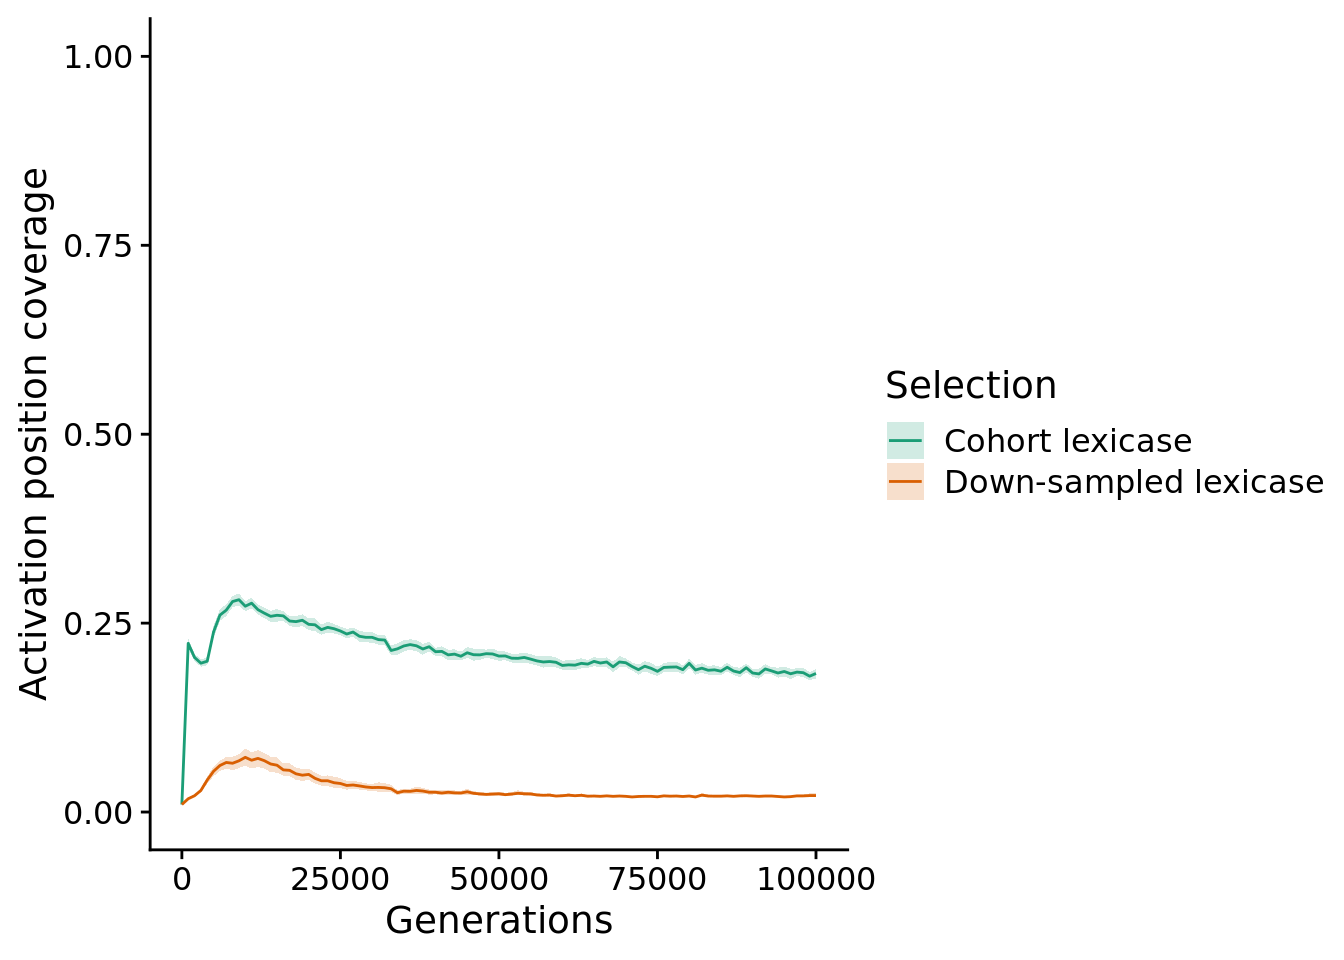
\includegraphics{supplemental-material_files/figure-latex/unnamed-chunk-76-1.pdf}

\hypertarget{final-starting-position-coverage-5}{%
\subsection{Final starting position coverage}\label{final-starting-position-coverage-5}}

\begin{Shaded}
\begin{Highlighting}[]
\CommentTok{# Compute manual labels for geom_signif}
\NormalTok{stat.test <-}\StringTok{ }\NormalTok{final_data }\OperatorTok
\StringTok{  }\KeywordTok{wilcox_test}\NormalTok{(unique_start_positions_coverage }\OperatorTok{~}\StringTok{ }\NormalTok{selection_name) }\OperatorTok
\StringTok{  }\KeywordTok{adjust_pvalue}\NormalTok{(}\DataTypeTok{method =} \StringTok{"bonferroni"}\NormalTok{) }\OperatorTok
\StringTok{  }\KeywordTok{add_significance}\NormalTok{() }\OperatorTok
\StringTok{  }\KeywordTok{add_xy_position}\NormalTok{(}\DataTypeTok{x=}\StringTok{"selection_name"}\NormalTok{,}\DataTypeTok{step.increase=}\DecValTok{1}\NormalTok{)}
\NormalTok{stat.test}\OperatorTok{$}\NormalTok{manual_position <-}\StringTok{ }\NormalTok{stat.test}\OperatorTok{$}\NormalTok{y.position }\OperatorTok{*}\StringTok{ }\FloatTok{1.05}
\NormalTok{stat.test}\OperatorTok{$}\NormalTok{label <-}\StringTok{ }\KeywordTok{mapply}\NormalTok{(p_label,stat.test}\OperatorTok{$}\NormalTok{p.adj)}
\end{Highlighting}
\end{Shaded}

\begin{Shaded}
\begin{Highlighting}[]
\NormalTok{unique_start_positions_coverage_final_fig <-}\StringTok{ }\KeywordTok{ggplot}\NormalTok{(}
\NormalTok{    final_data,}
    \KeywordTok{aes}\NormalTok{(}
      \DataTypeTok{x=}\NormalTok{selection_name,}
      \DataTypeTok{y=}\NormalTok{unique_start_positions_coverage,}
      \DataTypeTok{fill=}\NormalTok{selection_name}
\NormalTok{    )}
\NormalTok{  ) }\OperatorTok{+}
\StringTok{  }\KeywordTok{geom_flat_violin}\NormalTok{(}
    \DataTypeTok{position =} \KeywordTok{position_nudge}\NormalTok{(}\DataTypeTok{x =} \FloatTok{.2}\NormalTok{, }\DataTypeTok{y =} \DecValTok{0}\NormalTok{),}
    \DataTypeTok{alpha =} \FloatTok{.8}\NormalTok{,}
    \DataTypeTok{scale=}\StringTok{"width"}
\NormalTok{  ) }\OperatorTok{+}
\StringTok{  }\KeywordTok{geom_point}\NormalTok{(}
    \DataTypeTok{mapping=}\KeywordTok{aes}\NormalTok{(}\DataTypeTok{color=}\NormalTok{selection_name),}
    \DataTypeTok{position =} \KeywordTok{position_jitter}\NormalTok{(}\DataTypeTok{width =} \FloatTok{.15}\NormalTok{),}
    \DataTypeTok{size =} \FloatTok{.5}\NormalTok{,}
    \DataTypeTok{alpha =} \FloatTok{0.8}
\NormalTok{  ) }\OperatorTok{+}
\StringTok{  }\KeywordTok{geom_boxplot}\NormalTok{(}
    \DataTypeTok{width =} \FloatTok{.1}\NormalTok{,}
    \DataTypeTok{outlier.shape =} \OtherTok{NA}\NormalTok{,}
    \DataTypeTok{alpha =} \FloatTok{0.5}
\NormalTok{  ) }\OperatorTok{+}
\StringTok{  }\KeywordTok{scale_y_continuous}\NormalTok{(}
    \DataTypeTok{name=}\StringTok{"Activation position coverage"}\NormalTok{,}
    \DataTypeTok{limits=}\KeywordTok{c}\NormalTok{(}\DecValTok{0}\NormalTok{, }\FloatTok{1.0}\NormalTok{)}
\NormalTok{  ) }\OperatorTok{+}
\StringTok{  }\KeywordTok{scale_x_discrete}\NormalTok{(}
    \DataTypeTok{name=}\StringTok{"Selection"}\NormalTok{,}
    \DataTypeTok{limits=}\KeywordTok{c}\NormalTok{(}\StringTok{"CohortLexicase"}\NormalTok{, }\StringTok{"DownSampledLexicase"}\NormalTok{),}
    \DataTypeTok{labels=}\KeywordTok{c}\NormalTok{(}\StringTok{"Cohort lexicase"}\NormalTok{, }\StringTok{"Down-sampled lexicase"}\NormalTok{)}
\NormalTok{  ) }\OperatorTok{+}
\StringTok{  }\KeywordTok{scale_fill_brewer}\NormalTok{(}
    \DataTypeTok{name=}\StringTok{"Selection"}\NormalTok{,}
    \DataTypeTok{palette=}\NormalTok{cb_palette,}
    \DataTypeTok{limits=}\KeywordTok{c}\NormalTok{(}\StringTok{"CohortLexicase"}\NormalTok{, }\StringTok{"DownSampledLexicase"}\NormalTok{),}
    \DataTypeTok{labels=}\KeywordTok{c}\NormalTok{(}\StringTok{"Cohort lexicase"}\NormalTok{, }\StringTok{"Down-sampled lexicase"}\NormalTok{)}
\NormalTok{  ) }\OperatorTok{+}
\StringTok{  }\KeywordTok{scale_color_brewer}\NormalTok{(}
    \DataTypeTok{name=}\StringTok{"Selection"}\NormalTok{,}
    \DataTypeTok{palette=}\NormalTok{cb_palette,}
    \DataTypeTok{limits=}\KeywordTok{c}\NormalTok{(}\StringTok{"CohortLexicase"}\NormalTok{, }\StringTok{"DownSampledLexicase"}\NormalTok{),}
    \DataTypeTok{labels=}\KeywordTok{c}\NormalTok{(}\StringTok{"Cohort lexicase"}\NormalTok{, }\StringTok{"Down-sampled lexicase"}\NormalTok{)}
\NormalTok{  ) }\OperatorTok{+}
\StringTok{  }\KeywordTok{theme}\NormalTok{(}
    \DataTypeTok{legend.position=}\StringTok{"none"}
\NormalTok{  )}
\NormalTok{unique_start_positions_coverage_final_fig}
\end{Highlighting}
\end{Shaded}

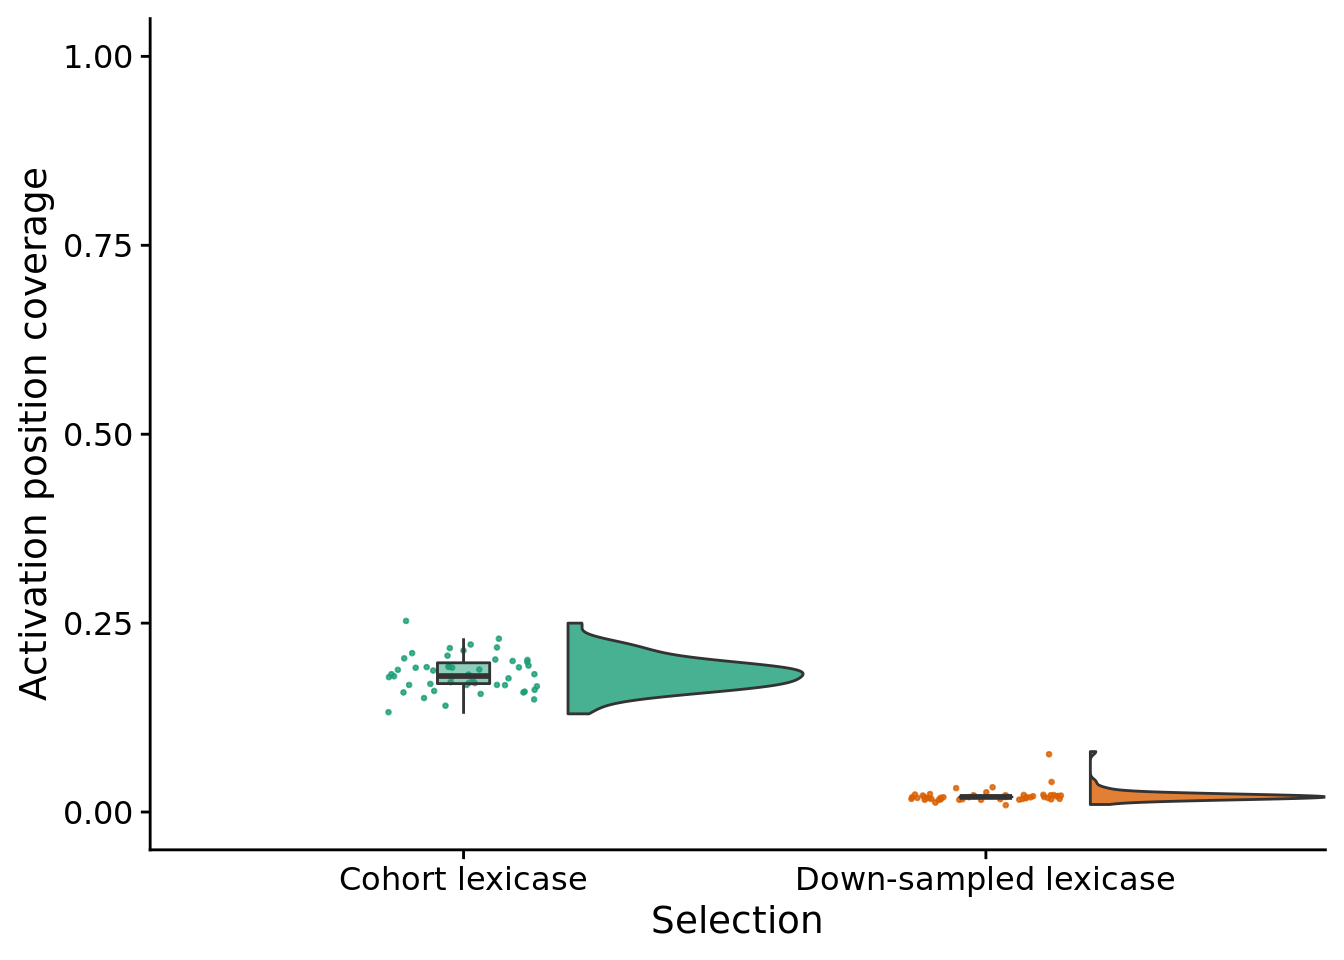
\includegraphics{supplemental-material_files/figure-latex/unnamed-chunk-78-1.pdf}

\begin{tabular}{l|l|l|r|r|r|r|r|l|r|l|r|r|r|l}
\hline
.y. & group1 & group2 & n1 & n2 & statistic & p & p.adj & p.adj.signif & y.position & groups & xmin & xmax & manual\_position & label\\
\hline
unique\_start\_positions\_coverage & CohortLexicase & DownSampledLexicase & 50 & 50 & 2500 & 0 & 0 & **** & 0.42 & CohortLexicase     , DownSampledLexicase & 1 & 2 & 0.441 & p < 1e-04\\
\hline
\end{tabular}

\hypertarget{manuscript-figures-6}{%
\section{Manuscript figures}\label{manuscript-figures-6}}

\begin{Shaded}
\begin{Highlighting}[]
\NormalTok{legend <-}\StringTok{ }\NormalTok{cowplot}\OperatorTok{::}\KeywordTok{get_legend}\NormalTok{(}
\NormalTok{    elite_ave_performance_fig }\OperatorTok{+}
\StringTok{      }\KeywordTok{guides}\NormalTok{(}
        \DataTypeTok{color=}\KeywordTok{guide_legend}\NormalTok{(}\DataTypeTok{nrow=}\DecValTok{1}\NormalTok{),}
        \DataTypeTok{fill=}\KeywordTok{guide_legend}\NormalTok{(}\DataTypeTok{nrow=}\DecValTok{1}\NormalTok{)}
\NormalTok{      ) }\OperatorTok{+}
\StringTok{      }\KeywordTok{theme}\NormalTok{(}
        \DataTypeTok{legend.position =} \StringTok{"bottom"}\NormalTok{,}
        \DataTypeTok{legend.box=}\StringTok{"horizontal"}\NormalTok{,}
        \DataTypeTok{legend.justification=}\StringTok{"center"}
\NormalTok{      )}
\NormalTok{  )}

\NormalTok{grid <-}\StringTok{ }\KeywordTok{plot_grid}\NormalTok{(}
\NormalTok{  elite_ave_performance_fig }\OperatorTok{+}
\StringTok{    }\KeywordTok{ggtitle}\NormalTok{(}\StringTok{"Performance over time"}\NormalTok{) }\OperatorTok{+}
\StringTok{    }\KeywordTok{theme}\NormalTok{(}\DataTypeTok{legend.position=}\StringTok{"none"}\NormalTok{),}
\NormalTok{  elite_final_performance_fig }\OperatorTok{+}
\StringTok{    }\KeywordTok{ggtitle}\NormalTok{(}\StringTok{"Final performance"}\NormalTok{) }\OperatorTok{+}
\StringTok{    }\KeywordTok{theme}\NormalTok{(),}
\NormalTok{  unique_start_position_coverage_fig }\OperatorTok{+}
\StringTok{    }\KeywordTok{ggtitle}\NormalTok{(}\StringTok{"Activation position coverage over time"}\NormalTok{) }\OperatorTok{+}
\StringTok{    }\KeywordTok{theme}\NormalTok{(}\DataTypeTok{legend.position=}\StringTok{"none"}\NormalTok{),}
\NormalTok{  unique_start_positions_coverage_final_fig }\OperatorTok{+}
\StringTok{    }\KeywordTok{ggtitle}\NormalTok{(}\StringTok{"Final activation position coverage"}\NormalTok{) }\OperatorTok{+}
\StringTok{    }\KeywordTok{theme}\NormalTok{(),}
  \DataTypeTok{nrow=}\DecValTok{2}\NormalTok{,}
  \DataTypeTok{ncol=}\DecValTok{2}\NormalTok{,}
  \DataTypeTok{rel_widths=}\KeywordTok{c}\NormalTok{(}\DecValTok{3}\NormalTok{,}\DecValTok{2}\NormalTok{),}
  \DataTypeTok{labels=}\StringTok{"auto"}
\NormalTok{)}

\NormalTok{grid <-}\StringTok{ }\KeywordTok{plot_grid}\NormalTok{(}
\NormalTok{  grid,}
\NormalTok{  legend,}
  \DataTypeTok{nrow=}\DecValTok{2}\NormalTok{,}
  \DataTypeTok{ncol=}\DecValTok{1}\NormalTok{,}
  \DataTypeTok{rel_heights=}\KeywordTok{c}\NormalTok{(}\DecValTok{1}\NormalTok{, }\FloatTok{0.1}\NormalTok{)}
\NormalTok{)}

\KeywordTok{save_plot}\NormalTok{(}
  \KeywordTok{paste}\NormalTok{(}
\NormalTok{    working_directory,}
    \StringTok{"imgs/down-sampled-vs-cohort-panel.pdf"}\NormalTok{,}
    \DataTypeTok{sep=}\StringTok{""}
\NormalTok{  ),}
\NormalTok{  grid,}
  \DataTypeTok{base_width=}\DecValTok{12}\NormalTok{,}
  \DataTypeTok{base_height=}\DecValTok{8}
\NormalTok{)}

\NormalTok{grid}
\end{Highlighting}
\end{Shaded}

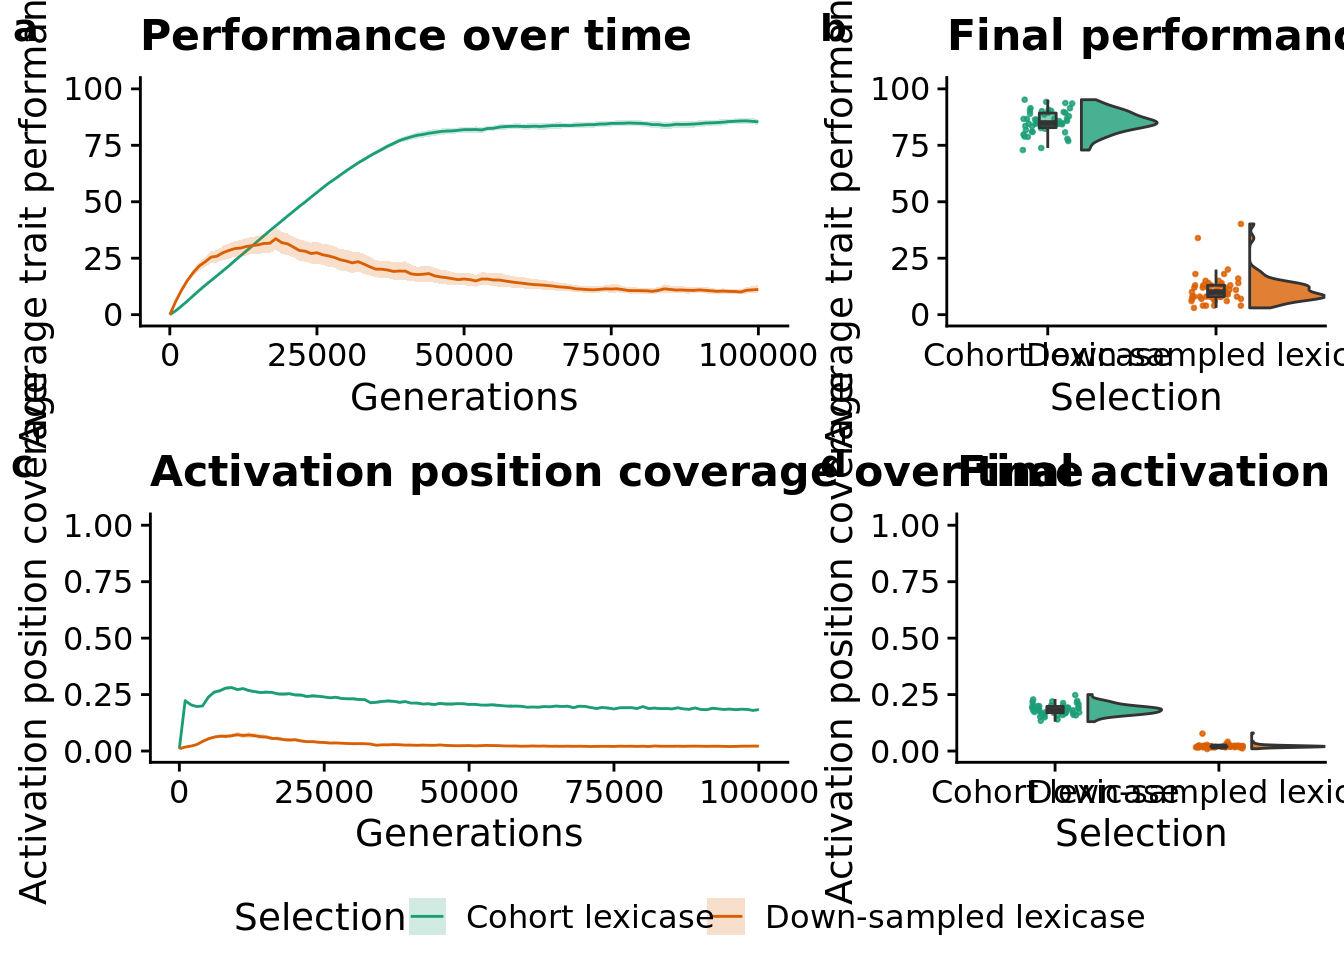
\includegraphics{supplemental-material_files/figure-latex/unnamed-chunk-80-1.pdf}

\hypertarget{novelty-lexicase}{%
\chapter{Novelty lexicase}\label{novelty-lexicase}}

\hypertarget{overview-7}{%
\section{Overview}\label{overview-7}}

\begin{Shaded}
\begin{Highlighting}[]
\CommentTok{# Relative location of data.}
\NormalTok{working_directory <-}\StringTok{ "experiments/2021-06-01-novelty/analysis/"}
\CommentTok{# working_directory <- "./"}

\CommentTok{# Settings for visualization}
\NormalTok{cb_palette <-}\StringTok{ "Set2"}
\CommentTok{# Create directory to dump plots}
\KeywordTok{dir.create}\NormalTok{(}\KeywordTok{paste0}\NormalTok{(working_directory, }\StringTok{"imgs"}\NormalTok{), }\DataTypeTok{showWarnings=}\OtherTok{FALSE}\NormalTok{)}
\end{Highlighting}
\end{Shaded}

\hypertarget{analysis-dependencies-7}{%
\section{Analysis dependencies}\label{analysis-dependencies-7}}

\begin{Shaded}
\begin{Highlighting}[]
\KeywordTok{library}\NormalTok{(ggplot2)}
\KeywordTok{library}\NormalTok{(tidyverse)}
\KeywordTok{library}\NormalTok{(cowplot)}
\KeywordTok{library}\NormalTok{(viridis)}
\KeywordTok{library}\NormalTok{(RColorBrewer)}
\KeywordTok{source}\NormalTok{(}\StringTok{"https://gist.githubusercontent.com/benmarwick/2a1bb0133ff568cbe28d/raw/fb53bd97121f7f9ce947837ef1a4c65a73bffb3f/geom_flat_violin.R"}\NormalTok{)}
\end{Highlighting}
\end{Shaded}

These analyses were conducted in the following computing environment:

\begin{Shaded}
\begin{Highlighting}[]
\KeywordTok{print}\NormalTok{(version)}
\end{Highlighting}
\end{Shaded}

\begin{verbatim}
##                _                           
## platform       x86_64-pc-linux-gnu         
## arch           x86_64                      
## os             linux-gnu                   
## system         x86_64, linux-gnu           
## status                                     
## major          4                           
## minor          1.0                         
## year           2021                        
## month          05                          
## day            18                          
## svn rev        80317                       
## language       R                           
## version.string R version 4.1.0 (2021-05-18)
## nickname       Camp Pontanezen
\end{verbatim}

\hypertarget{setup-7}{%
\section{Setup}\label{setup-7}}

\begin{Shaded}
\begin{Highlighting}[]
\NormalTok{data_loc <-}\StringTok{ }\KeywordTok{paste0}\NormalTok{(}
\NormalTok{  working_directory,}
  \StringTok{"data/timeseries-res-1000g.csv"}
\NormalTok{)}

\NormalTok{data <-}\StringTok{ }\KeywordTok{read.csv}\NormalTok{(data_loc, }\DataTypeTok{na.strings=}\StringTok{"NONE"}\NormalTok{)}

\NormalTok{data}\OperatorTok{$}\NormalTok{cardinality <-}\StringTok{ }\KeywordTok{as.factor}\NormalTok{(}
\NormalTok{  data}\OperatorTok{$}\NormalTok{OBJECTIVE_CNT}
\NormalTok{)}
\NormalTok{data}\OperatorTok{$}\NormalTok{selection_name <-}\StringTok{ }\KeywordTok{as.factor}\NormalTok{(}
\NormalTok{  data}\OperatorTok{$}\NormalTok{selection_name}
\NormalTok{)}

\NormalTok{data}\OperatorTok{$}\NormalTok{epsilon <-}\StringTok{ }\KeywordTok{as.factor}\NormalTok{(}
\NormalTok{  data}\OperatorTok{$}\NormalTok{LEX_EPS}
\NormalTok{)}

\NormalTok{data}\OperatorTok{$}\NormalTok{k <-}\StringTok{ }\KeywordTok{as.factor}\NormalTok{(}
\NormalTok{   data}\OperatorTok{$}\NormalTok{NOVEL_K}
\NormalTok{)}

\NormalTok{data}\OperatorTok{$}\NormalTok{elite_trait_avg <-}
\StringTok{  }\NormalTok{data}\OperatorTok{$}\NormalTok{ele_agg_per }\OperatorTok{/}\StringTok{ }\NormalTok{data}\OperatorTok{$}\NormalTok{OBJECTIVE_CNT}
\NormalTok{data}\OperatorTok{$}\NormalTok{unique_start_positions_coverage <-}
\StringTok{  }\NormalTok{data}\OperatorTok{$}\NormalTok{uni_str_pos }\OperatorTok{/}\StringTok{ }\NormalTok{data}\OperatorTok{$}\NormalTok{OBJECTIVE_CNT}

\NormalTok{final_data <-}\StringTok{ }\KeywordTok{filter}\NormalTok{(data, evaluations}\OperatorTok{==}\KeywordTok{max}\NormalTok{(data}\OperatorTok{$}\NormalTok{evaluations))}

\CommentTok{####### misc #######}
\CommentTok{# Configure our default graphing theme}
\KeywordTok{theme_set}\NormalTok{(}\KeywordTok{theme_cowplot}\NormalTok{())}
\end{Highlighting}
\end{Shaded}

\hypertarget{exploration-diagnostic-performance-7}{%
\section{Exploration diagnostic performance}\label{exploration-diagnostic-performance-7}}

\begin{Shaded}
\begin{Highlighting}[]
\NormalTok{elite_ave_performance_fig <-}
\StringTok{  }\KeywordTok{ggplot}\NormalTok{(}
\NormalTok{    data,}
    \KeywordTok{aes}\NormalTok{(}\DataTypeTok{x=}\NormalTok{gen, }\DataTypeTok{y=}\NormalTok{elite_trait_avg, }\DataTypeTok{color=}\NormalTok{k, }\DataTypeTok{fill=}\NormalTok{k)}
\NormalTok{  ) }\OperatorTok{+}
\StringTok{  }\KeywordTok{stat_summary}\NormalTok{(}\DataTypeTok{geom=}\StringTok{"line"}\NormalTok{, }\DataTypeTok{fun=}\NormalTok{mean) }\OperatorTok{+}
\StringTok{  }\KeywordTok{stat_summary}\NormalTok{(}
    \DataTypeTok{geom=}\StringTok{"ribbon"}\NormalTok{,}
    \DataTypeTok{fun.data=}\StringTok{"mean_cl_boot"}\NormalTok{,}
    \DataTypeTok{fun.args=}\KeywordTok{list}\NormalTok{(}\DataTypeTok{conf.int=}\FloatTok{0.95}\NormalTok{),}
    \DataTypeTok{alpha=}\FloatTok{0.2}\NormalTok{,}
    \DataTypeTok{linetype=}\DecValTok{0}
\NormalTok{  ) }\OperatorTok{+}
\StringTok{  }\KeywordTok{scale_y_continuous}\NormalTok{(}
    \DataTypeTok{name=}\StringTok{"Average trait performance"}\NormalTok{,}
    \DataTypeTok{limits=}\KeywordTok{c}\NormalTok{(}\DecValTok{0}\NormalTok{, }\DecValTok{100}\NormalTok{)}
\NormalTok{  ) }\OperatorTok{+}
\StringTok{  }\KeywordTok{scale_x_continuous}\NormalTok{(}
    \DataTypeTok{name=}\StringTok{"Generations"}
\NormalTok{  ) }\OperatorTok{+}
\StringTok{  }\KeywordTok{scale_fill_brewer}\NormalTok{(}
    \DataTypeTok{name=}\StringTok{"k"}\NormalTok{,}
    \DataTypeTok{palette=}\NormalTok{cb_palette}
\NormalTok{  ) }\OperatorTok{+}
\StringTok{  }\KeywordTok{scale_color_brewer}\NormalTok{(}
    \DataTypeTok{name=}\StringTok{"k"}\NormalTok{,}
    \DataTypeTok{palette=}\NormalTok{cb_palette}
\NormalTok{  )}
\NormalTok{elite_ave_performance_fig}
\end{Highlighting}
\end{Shaded}

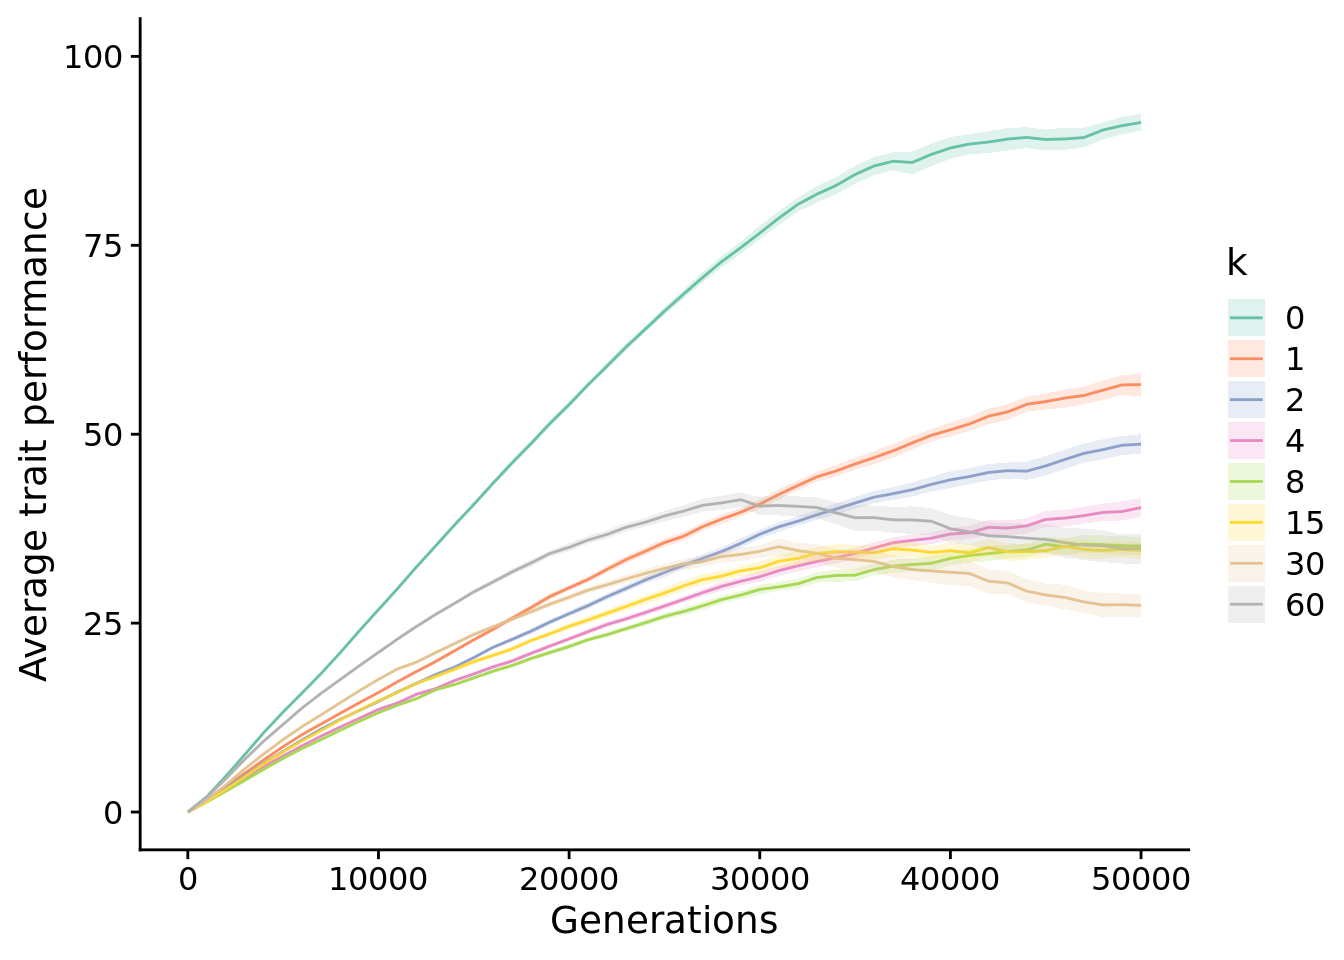
\includegraphics{supplemental-material_files/figure-latex/unnamed-chunk-85-1.pdf}

\hypertarget{final-performance-7}{%
\subsection{Final performance}\label{final-performance-7}}

\begin{Shaded}
\begin{Highlighting}[]
\NormalTok{elite_final_performance_fig <-}\StringTok{ }\KeywordTok{ggplot}\NormalTok{(}
\NormalTok{    final_data,}
    \KeywordTok{aes}\NormalTok{(}\DataTypeTok{x=}\NormalTok{k, }\DataTypeTok{y=}\NormalTok{elite_trait_avg, }\DataTypeTok{fill=}\NormalTok{k)}
\NormalTok{  ) }\OperatorTok{+}
\StringTok{  }\KeywordTok{geom_flat_violin}\NormalTok{(}
    \DataTypeTok{position =} \KeywordTok{position_nudge}\NormalTok{(}\DataTypeTok{x =} \FloatTok{.2}\NormalTok{, }\DataTypeTok{y =} \DecValTok{0}\NormalTok{),}
    \DataTypeTok{alpha =} \FloatTok{.8}\NormalTok{,}
    \DataTypeTok{scale=}\StringTok{"width"}
\NormalTok{  ) }\OperatorTok{+}
\StringTok{  }\KeywordTok{geom_point}\NormalTok{(}
    \DataTypeTok{mapping=}\KeywordTok{aes}\NormalTok{(}\DataTypeTok{color=}\NormalTok{k),}
    \DataTypeTok{position =} \KeywordTok{position_jitter}\NormalTok{(}\DataTypeTok{width =} \FloatTok{.15}\NormalTok{),}
    \DataTypeTok{size =} \FloatTok{.5}\NormalTok{,}
    \DataTypeTok{alpha =} \FloatTok{0.8}
\NormalTok{  ) }\OperatorTok{+}
\StringTok{  }\KeywordTok{geom_boxplot}\NormalTok{(}
    \DataTypeTok{width =} \FloatTok{.1}\NormalTok{,}
    \DataTypeTok{outlier.shape =} \OtherTok{NA}\NormalTok{,}
    \DataTypeTok{alpha =} \FloatTok{0.5}
\NormalTok{  ) }\OperatorTok{+}
\StringTok{  }\KeywordTok{scale_y_continuous}\NormalTok{(}
    \DataTypeTok{name=}\StringTok{"Average trait performance"}\NormalTok{,}
    \DataTypeTok{limits=}\KeywordTok{c}\NormalTok{(}\DecValTok{0}\NormalTok{, }\DecValTok{100}\NormalTok{)}
\NormalTok{  ) }\OperatorTok{+}
\StringTok{  }\KeywordTok{scale_x_discrete}\NormalTok{(}
    \DataTypeTok{name=}\StringTok{"k"}
\NormalTok{  ) }\OperatorTok{+}
\StringTok{  }\KeywordTok{scale_fill_brewer}\NormalTok{(}
    \DataTypeTok{name=}\StringTok{"k"}\NormalTok{,}
    \DataTypeTok{palette=}\NormalTok{cb_palette}
\NormalTok{  ) }\OperatorTok{+}
\StringTok{  }\KeywordTok{scale_color_brewer}\NormalTok{(}
    \DataTypeTok{name=}\StringTok{"k"}\NormalTok{,}
    \DataTypeTok{palette=}\NormalTok{cb_palette}
\NormalTok{  ) }\OperatorTok{+}
\StringTok{  }\KeywordTok{theme}\NormalTok{(}
    \DataTypeTok{legend.position=}\StringTok{"none"}
\NormalTok{  )}
\NormalTok{elite_final_performance_fig}
\end{Highlighting}
\end{Shaded}

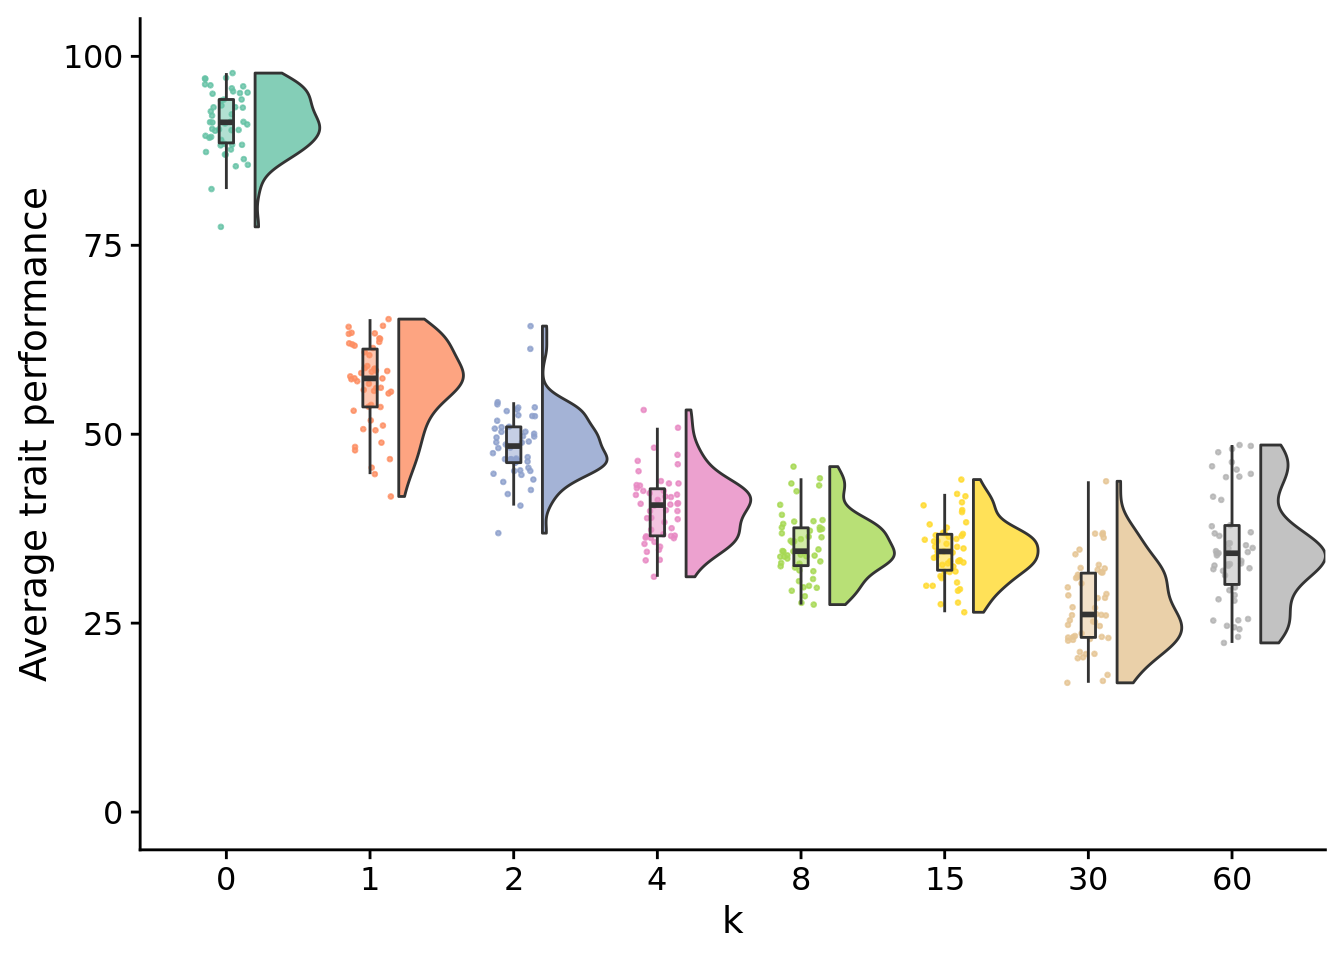
\includegraphics{supplemental-material_files/figure-latex/unnamed-chunk-86-1.pdf}

\hypertarget{unique-starting-positions-7}{%
\section{Unique starting positions}\label{unique-starting-positions-7}}

\begin{Shaded}
\begin{Highlighting}[]
\NormalTok{unique_start_position_coverage_fig <-}\StringTok{ }\KeywordTok{ggplot}\NormalTok{(}
\NormalTok{    data,}
    \KeywordTok{aes}\NormalTok{(}\DataTypeTok{x=}\NormalTok{gen, }\DataTypeTok{y=}\NormalTok{unique_start_positions_coverage, }\DataTypeTok{color=}\NormalTok{k, }\DataTypeTok{fill=}\NormalTok{k)}
\NormalTok{  ) }\OperatorTok{+}
\StringTok{  }\KeywordTok{stat_summary}\NormalTok{(}\DataTypeTok{geom=}\StringTok{"line"}\NormalTok{, }\DataTypeTok{fun=}\NormalTok{mean) }\OperatorTok{+}
\StringTok{  }\KeywordTok{stat_summary}\NormalTok{(}
    \DataTypeTok{geom=}\StringTok{"ribbon"}\NormalTok{,}
    \DataTypeTok{fun.data=}\StringTok{"mean_cl_boot"}\NormalTok{,}
    \DataTypeTok{fun.args=}\KeywordTok{list}\NormalTok{(}\DataTypeTok{conf.int=}\FloatTok{0.95}\NormalTok{),}
    \DataTypeTok{alpha=}\FloatTok{0.2}\NormalTok{,}
    \DataTypeTok{linetype=}\DecValTok{0}
\NormalTok{  ) }\OperatorTok{+}
\StringTok{  }\KeywordTok{scale_y_continuous}\NormalTok{(}
    \DataTypeTok{name=}\StringTok{"Activation position coverage"}\NormalTok{,}
    \DataTypeTok{limits=}\KeywordTok{c}\NormalTok{(}\FloatTok{0.0}\NormalTok{, }\FloatTok{1.0}\NormalTok{)}
\NormalTok{  ) }\OperatorTok{+}
\StringTok{  }\KeywordTok{scale_x_continuous}\NormalTok{(}
    \DataTypeTok{name=}\StringTok{"Generations"}
\NormalTok{  ) }\OperatorTok{+}
\StringTok{  }\KeywordTok{scale_fill_brewer}\NormalTok{(}
    \DataTypeTok{name=}\StringTok{"k"}\NormalTok{,}
    \DataTypeTok{palette=}\NormalTok{cb_palette}
\NormalTok{  ) }\OperatorTok{+}
\StringTok{  }\KeywordTok{scale_color_brewer}\NormalTok{(}
    \DataTypeTok{name=}\StringTok{"k"}\NormalTok{,}
    \DataTypeTok{palette=}\NormalTok{cb_palette}
\NormalTok{  )}
\NormalTok{unique_start_position_coverage_fig}
\end{Highlighting}
\end{Shaded}

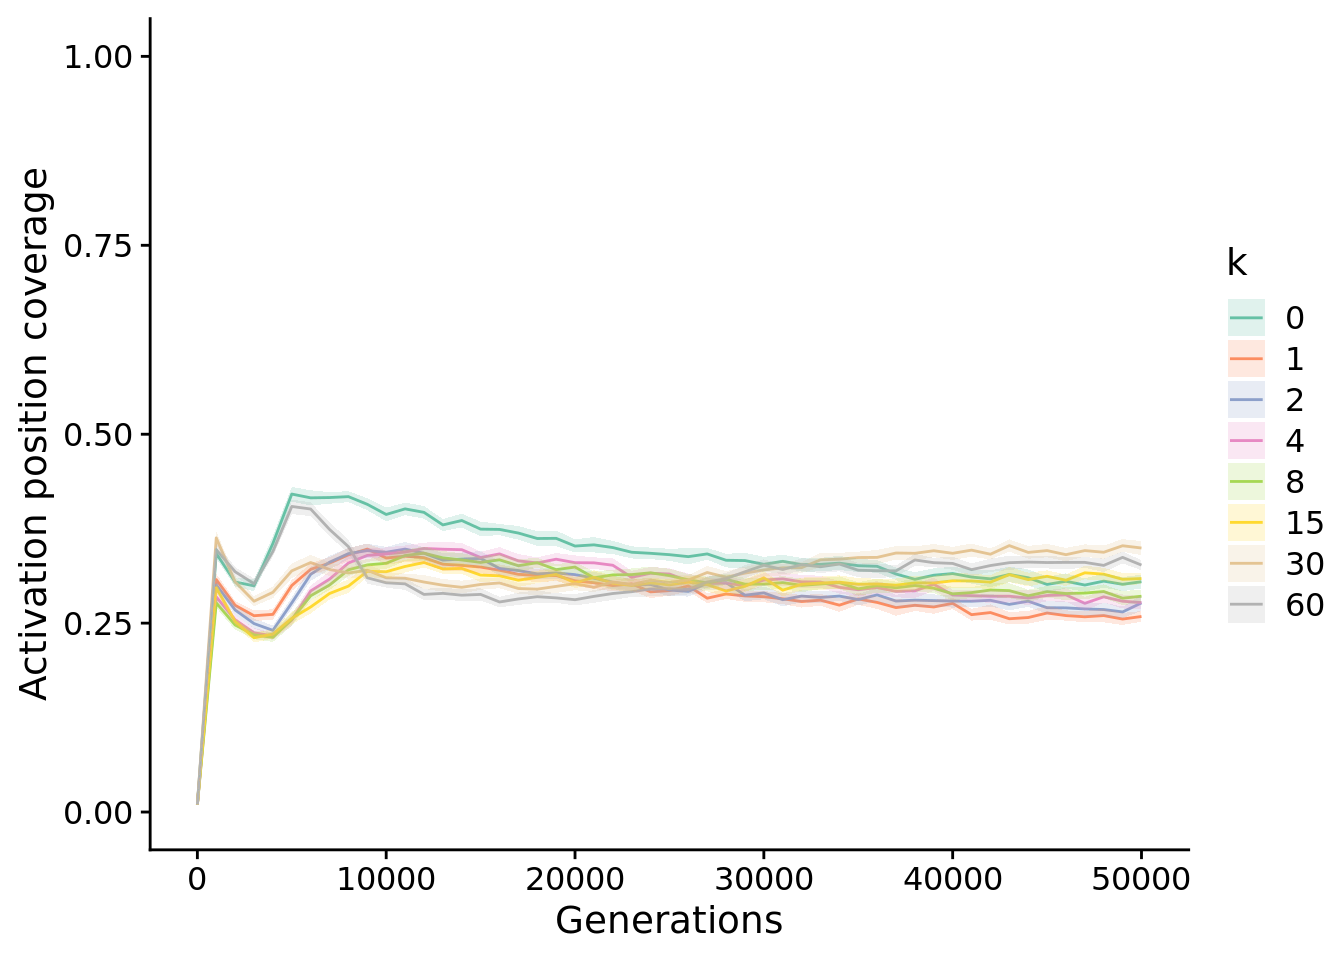
\includegraphics{supplemental-material_files/figure-latex/unnamed-chunk-87-1.pdf}

\hypertarget{final-starting-position-coverage-6}{%
\subsection{Final starting position coverage}\label{final-starting-position-coverage-6}}

\begin{Shaded}
\begin{Highlighting}[]
\NormalTok{unique_start_positions_coverage_final_fig <-}\StringTok{ }\KeywordTok{ggplot}\NormalTok{(}
\NormalTok{    final_data,}
    \KeywordTok{aes}\NormalTok{(}\DataTypeTok{x=}\NormalTok{k, }\DataTypeTok{y=}\NormalTok{unique_start_positions_coverage, }\DataTypeTok{fill=}\NormalTok{k)}
\NormalTok{  ) }\OperatorTok{+}
\StringTok{  }\KeywordTok{geom_flat_violin}\NormalTok{(}
    \DataTypeTok{position =} \KeywordTok{position_nudge}\NormalTok{(}\DataTypeTok{x =} \FloatTok{.2}\NormalTok{, }\DataTypeTok{y =} \DecValTok{0}\NormalTok{),}
    \DataTypeTok{alpha =} \FloatTok{.8}\NormalTok{,}
    \DataTypeTok{scale=}\StringTok{"width"}
\NormalTok{  ) }\OperatorTok{+}
\StringTok{  }\KeywordTok{geom_point}\NormalTok{(}
    \DataTypeTok{mapping=}\KeywordTok{aes}\NormalTok{(}\DataTypeTok{color=}\NormalTok{k),}
    \DataTypeTok{position =} \KeywordTok{position_jitter}\NormalTok{(}\DataTypeTok{width =} \FloatTok{.15}\NormalTok{),}
    \DataTypeTok{size =} \FloatTok{.5}\NormalTok{,}
    \DataTypeTok{alpha =} \FloatTok{0.8}
\NormalTok{  ) }\OperatorTok{+}
\StringTok{  }\KeywordTok{geom_boxplot}\NormalTok{(}
    \DataTypeTok{width =} \FloatTok{.1}\NormalTok{,}
    \DataTypeTok{outlier.shape =} \OtherTok{NA}\NormalTok{,}
    \DataTypeTok{alpha =} \FloatTok{0.5}
\NormalTok{  ) }\OperatorTok{+}
\StringTok{  }\KeywordTok{scale_y_continuous}\NormalTok{(}
    \DataTypeTok{name=}\StringTok{"Activation position coverage"}\NormalTok{,}
    \DataTypeTok{limits=}\KeywordTok{c}\NormalTok{(}\DecValTok{0}\NormalTok{, }\FloatTok{1.0}\NormalTok{)}
\NormalTok{  ) }\OperatorTok{+}
\StringTok{  }\KeywordTok{scale_x_discrete}\NormalTok{(}
    \DataTypeTok{name=}\StringTok{"k"}
\NormalTok{  ) }\OperatorTok{+}
\StringTok{  }\KeywordTok{scale_fill_brewer}\NormalTok{(}
    \DataTypeTok{name=}\StringTok{"k"}\NormalTok{,}
    \DataTypeTok{palette=}\NormalTok{cb_palette}
\NormalTok{  ) }\OperatorTok{+}
\StringTok{  }\KeywordTok{scale_color_brewer}\NormalTok{(}
    \DataTypeTok{name=}\StringTok{"k"}\NormalTok{,}
    \DataTypeTok{palette=}\NormalTok{cb_palette}
\NormalTok{  ) }\OperatorTok{+}
\StringTok{  }\KeywordTok{theme}\NormalTok{(}
    \DataTypeTok{legend.position=}\StringTok{"none"}
\NormalTok{  )}
\NormalTok{unique_start_positions_coverage_final_fig}
\end{Highlighting}
\end{Shaded}

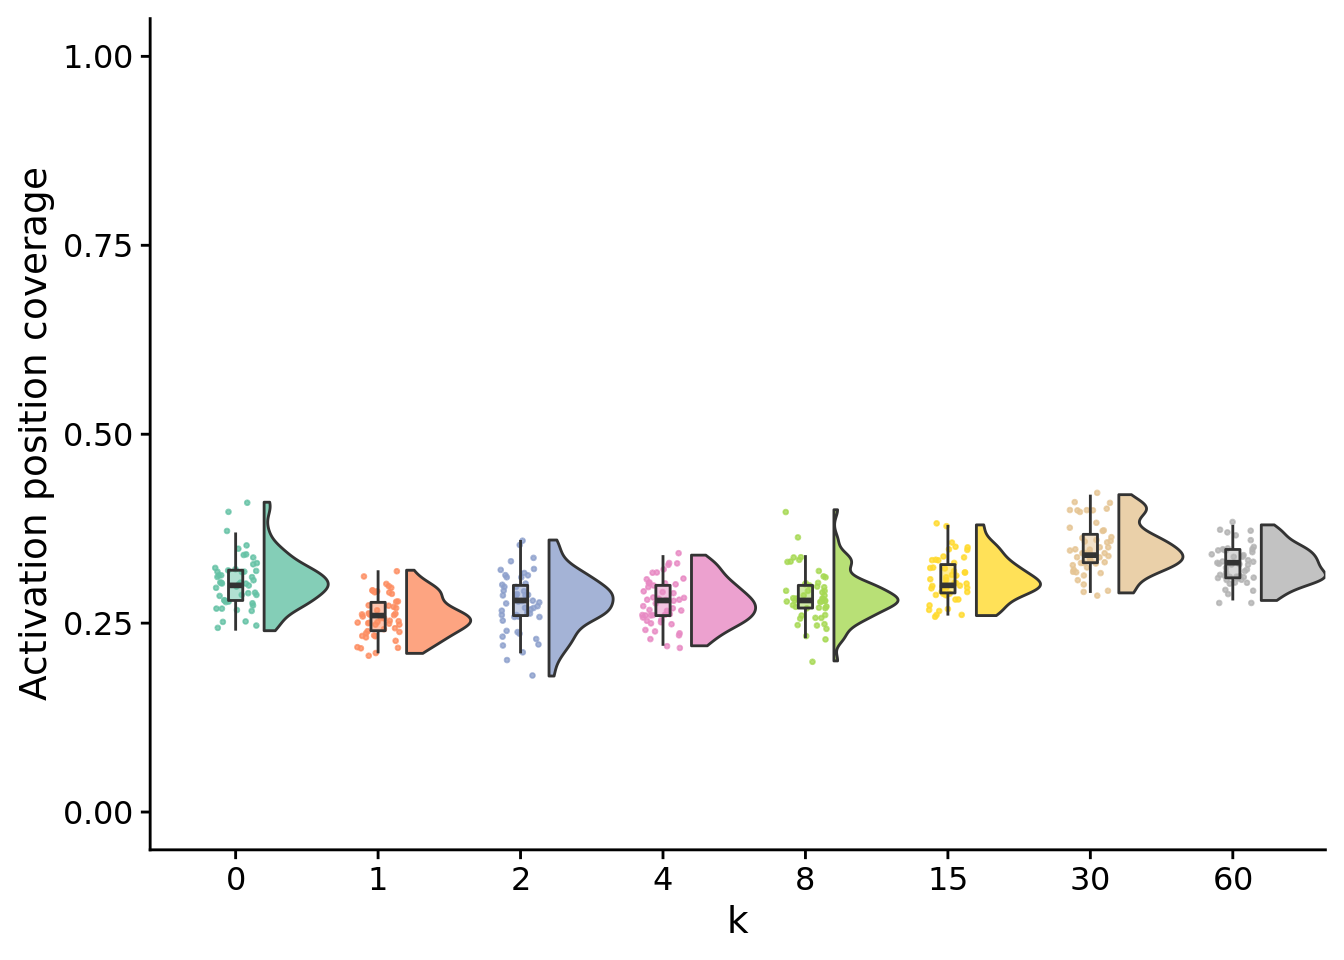
\includegraphics{supplemental-material_files/figure-latex/unnamed-chunk-88-1.pdf}

\hypertarget{manuscript-figures-7}{%
\section{Manuscript figures}\label{manuscript-figures-7}}

\begin{Shaded}
\begin{Highlighting}[]
\NormalTok{legend <-}\StringTok{ }\NormalTok{cowplot}\OperatorTok{::}\KeywordTok{get_legend}\NormalTok{(}
\NormalTok{    elite_ave_performance_fig }\OperatorTok{+}
\StringTok{      }\KeywordTok{guides}\NormalTok{(}
        \DataTypeTok{color=}\KeywordTok{guide_legend}\NormalTok{(}\DataTypeTok{nrow=}\DecValTok{1}\NormalTok{),}
        \DataTypeTok{fill=}\KeywordTok{guide_legend}\NormalTok{(}\DataTypeTok{nrow=}\DecValTok{1}\NormalTok{)}
\NormalTok{      ) }\OperatorTok{+}
\StringTok{      }\KeywordTok{theme}\NormalTok{(}
        \DataTypeTok{legend.position =} \StringTok{"bottom"}\NormalTok{,}
        \DataTypeTok{legend.box=}\StringTok{"horizontal"}\NormalTok{,}
        \DataTypeTok{legend.justification=}\StringTok{"center"}
\NormalTok{      )}
\NormalTok{  )}

\NormalTok{grid <-}\StringTok{ }\KeywordTok{plot_grid}\NormalTok{(}
\NormalTok{  elite_ave_performance_fig }\OperatorTok{+}
\StringTok{    }\KeywordTok{ggtitle}\NormalTok{(}\StringTok{"Performance over time"}\NormalTok{) }\OperatorTok{+}
\StringTok{    }\KeywordTok{theme}\NormalTok{(}\DataTypeTok{legend.position=}\StringTok{"none"}\NormalTok{),}
\NormalTok{  elite_final_performance_fig }\OperatorTok{+}
\StringTok{    }\KeywordTok{ggtitle}\NormalTok{(}\StringTok{"Final performance"}\NormalTok{) }\OperatorTok{+}
\StringTok{    }\KeywordTok{theme}\NormalTok{(),}
\NormalTok{  unique_start_position_coverage_fig }\OperatorTok{+}
\StringTok{    }\KeywordTok{ggtitle}\NormalTok{(}\StringTok{"Activation position coverage over time"}\NormalTok{) }\OperatorTok{+}
\StringTok{    }\KeywordTok{theme}\NormalTok{(}\DataTypeTok{legend.position=}\StringTok{"none"}\NormalTok{),}
\NormalTok{  unique_start_positions_coverage_final_fig }\OperatorTok{+}
\StringTok{    }\KeywordTok{ggtitle}\NormalTok{(}\StringTok{"Final activation position coverage"}\NormalTok{) }\OperatorTok{+}
\StringTok{    }\KeywordTok{theme}\NormalTok{(),}
  \DataTypeTok{nrow=}\DecValTok{2}\NormalTok{,}
  \DataTypeTok{ncol=}\DecValTok{2}\NormalTok{,}
  \DataTypeTok{rel_widths=}\KeywordTok{c}\NormalTok{(}\DecValTok{3}\NormalTok{,}\DecValTok{2}\NormalTok{),}
  \DataTypeTok{labels=}\StringTok{"auto"}
\NormalTok{)}

\NormalTok{grid <-}\StringTok{ }\KeywordTok{plot_grid}\NormalTok{(}
\NormalTok{  grid,}
\NormalTok{  legend,}
  \DataTypeTok{nrow=}\DecValTok{2}\NormalTok{,}
  \DataTypeTok{ncol=}\DecValTok{1}\NormalTok{,}
  \DataTypeTok{rel_heights=}\KeywordTok{c}\NormalTok{(}\DecValTok{1}\NormalTok{, }\FloatTok{0.1}\NormalTok{)}
\NormalTok{)}

\KeywordTok{save_plot}\NormalTok{(}
  \KeywordTok{paste}\NormalTok{(working_directory, }\StringTok{"imgs/novelty-panel.pdf"}\NormalTok{, }\DataTypeTok{sep=}\StringTok{""}\NormalTok{),}
\NormalTok{  grid,}
  \DataTypeTok{base_width=}\DecValTok{12}\NormalTok{,}
  \DataTypeTok{base_height=}\DecValTok{8}
\NormalTok{)}

\NormalTok{grid}
\end{Highlighting}
\end{Shaded}

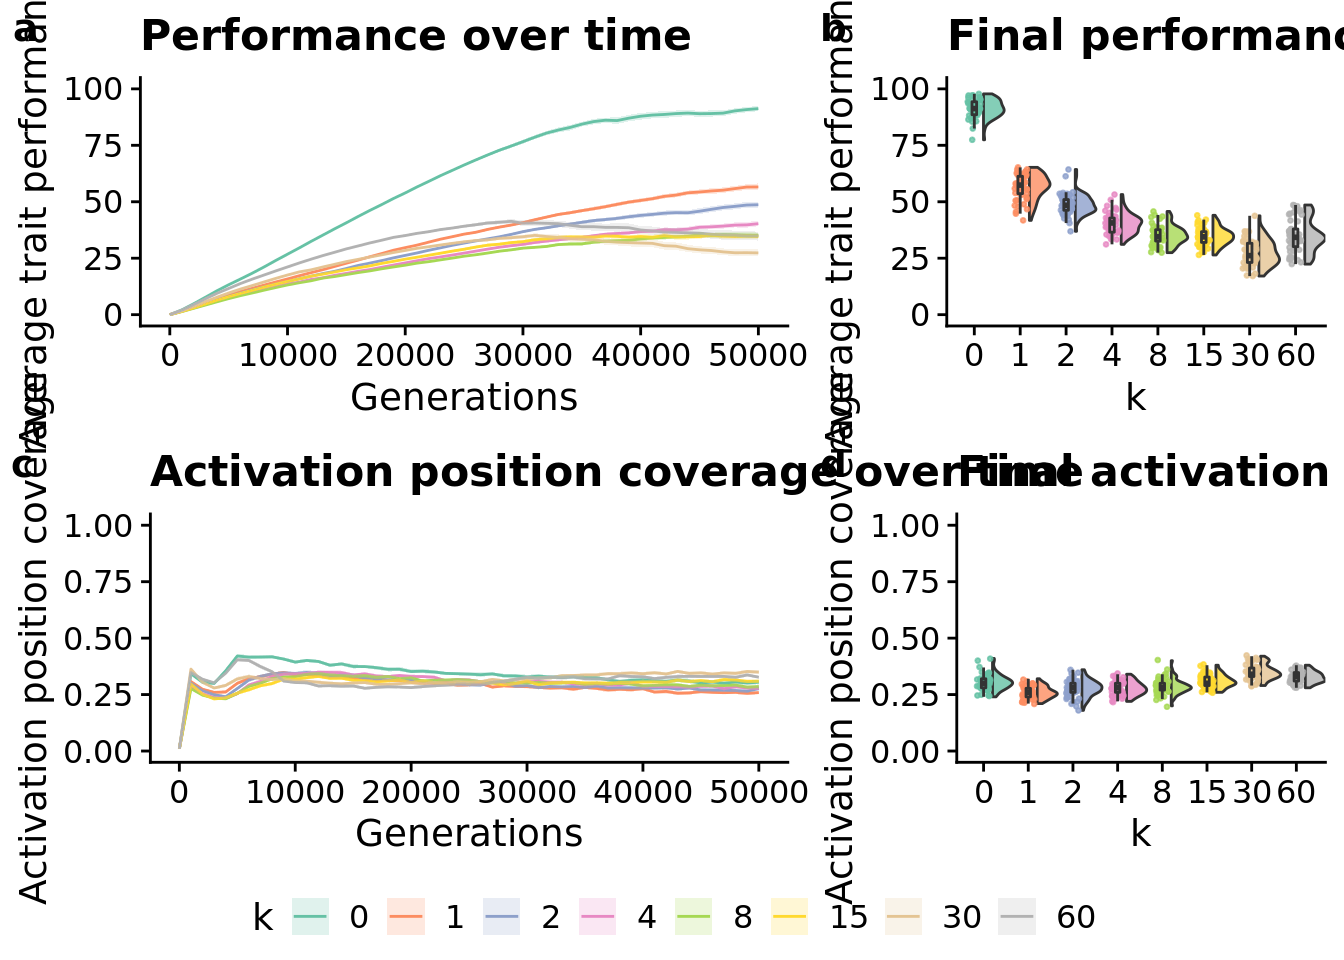
\includegraphics{supplemental-material_files/figure-latex/unnamed-chunk-89-1.pdf}

\bibliography{packages.bib,supplemental.bib}

\end{document}
